

\documentclass [
% 	draft		% falls ohne Bilder gedruckt werden soll (Entwurf)
	]{scrbook}	% KOMA Klasse für Bücher

%%MOD%%
\usepackage{fhacmb}	% Style-File für Titelblatt. Ggf. bei Enning holen

\KOMAoptions{
	parskip=true,		% Absätze mit Abstand
	fontsize=12pt,		% Standardschriftgröße
	toc=flat,		% Inhaltsverzeichnis ohne Einzüge
	twoside=false,		% Einseitig setzen
	numbers=nodotatend,	% Nummerierungen nicht mit Punkt abschließen
% die folgenden Optionen nehmen die entsprechende Dinge ins Inhaltsverzeichnis auf
% mit der bei texlive vorhandenen aktuellen Version von pdflatex funkioniert es nicht mehr
% (bekannter Bug)
	toc=bibliography,	% Literaturverzeichnis ins Inhaltsverzeichnis
	toc=listof,		% Abbildung- und Tabellenverzeichnis ins Inhaltsverzeichnis
	toc=index,		% Stichwortverzeichnis ins Inhaltsverzeichnis
	}
%

\usepackage{amsmath,amssymb}



\IfFileExists{xcolor.sty}{
    \RequirePackage{xcolor}
}{
    \RequirePackage{color}
}


\providecommand{\tightlist}{%
  \setlength{\itemsep}{0pt}\setlength{\parskip}{0pt}}



\usepackage{footnotebackref}
\usepackage{graphicx}






%%
%% added
%%

%
% language specification
%
% If no language is specified, use English as the default main document language.
%
%%MOD%%



%
% for the background color of the title page
%

%
% break urls
%
\PassOptionsToPackage{hyphens}{url}

%
% When using babel or polyglossia with biblatex, loading csquotes is recommended
% to ensure that quoted texts are typeset according to the rules of your main language.
%
\usepackage{csquotes}


%
% variables for title, author and date
%
\usepackage{titling}





%
% ADD SYNTAX HIGHLIGHTING
%

%
%
% Listings
%
%
\usepackage{listings}
\newcommand{\passthrough}[1]{#1}
\lstset{defaultdialect=[5.3]Lua}
\lstset{defaultdialect=[x86masm]Assembler}
%
% general listing colors
%
\definecolor{listing-background}{HTML}{F7F7F7}
\definecolor{listing-rule}{HTML}{B3B2B3}
\definecolor{listing-numbers}{HTML}{B3B2B3}
\definecolor{listing-text-color}{HTML}{000000}
\definecolor{listing-keyword}{HTML}{435489}
\definecolor{listing-keyword-2}{HTML}{1284CA} % additional keywords
\definecolor{listing-keyword-3}{HTML}{9137CB} % additional keywords
\definecolor{listing-identifier}{HTML}{435489}
\definecolor{listing-string}{HTML}{00999A}
\definecolor{listing-comment}{HTML}{8E8E8E}

\lstdefinestyle{eisvogel_listing_style}{
  language         = java,
  numbers          = left,
  xleftmargin      = 2.7em,
  framexleftmargin = 2.5em,
  backgroundcolor  = \color{listing-background},
  basicstyle       = \color{listing-text-color}\linespread{1.0}\small\ttfamily{},
  breaklines       = true,
  frame            = single,
  framesep         = 0.19em,
  rulecolor        = \color{listing-rule},
  frameround       = ffff,
  tabsize          = 4,
  numberstyle      = \color{listing-numbers},
  aboveskip        = 1.0em,
  belowskip        = 0.1em,
  abovecaptionskip = 0em,
  belowcaptionskip = 1.0em,
  keywordstyle     = {\color{listing-keyword}\bfseries},
  keywordstyle     = {[2]\color{listing-keyword-2}\bfseries},
  keywordstyle     = {[3]\color{listing-keyword-3}\bfseries\itshape},
  sensitive        = true,
  identifierstyle  = \color{listing-identifier},
  commentstyle     = \color{listing-comment},
  stringstyle      = \color{listing-string},
  showstringspaces = false,
  escapeinside     = {/*@}{@*/}, % Allow LaTeX inside these special comments
  literate         =
  {á}{{\'a}}1 {é}{{\'e}}1 {í}{{\'i}}1 {ó}{{\'o}}1 {ú}{{\'u}}1
  {Á}{{\'A}}1 {É}{{\'E}}1 {Í}{{\'I}}1 {Ó}{{\'O}}1 {Ú}{{\'U}}1
  {à}{{\`a}}1 {è}{{\'e}}1 {ì}{{\`i}}1 {ò}{{\`o}}1 {ù}{{\`u}}1
  {À}{{\`A}}1 {È}{{\'E}}1 {Ì}{{\`I}}1 {Ò}{{\`O}}1 {Ù}{{\`U}}1
  {ä}{{\"a}}1 {ë}{{\"e}}1 {ï}{{\"i}}1 {ö}{{\"o}}1 {ü}{{\"u}}1
  {Ä}{{\"A}}1 {Ë}{{\"E}}1 {Ï}{{\"I}}1 {Ö}{{\"O}}1 {Ü}{{\"U}}1
  {â}{{\^a}}1 {ê}{{\^e}}1 {î}{{\^i}}1 {ô}{{\^o}}1 {û}{{\^u}}1
  {Â}{{\^A}}1 {Ê}{{\^E}}1 {Î}{{\^I}}1 {Ô}{{\^O}}1 {Û}{{\^U}}1
  {œ}{{\oe}}1 {Œ}{{\OE}}1 {æ}{{\ae}}1 {Æ}{{\AE}}1 {ß}{{\ss}}1
  {ç}{{\c c}}1 {Ç}{{\c C}}1 {ø}{{\o}}1 {å}{{\r a}}1 {Å}{{\r A}}1
  {€}{{\EUR}}1 {£}{{\pounds}}1 {«}{{\guillemotleft}}1
  {»}{{\guillemotright}}1 {ñ}{{\~n}}1 {Ñ}{{\~N}}1 {¿}{{?`}}1
  {…}{{\ldots}}1 {≥}{{>=}}1 {≤}{{<=}}1 {„}{{\glqq}}1 {“}{{\grqq}}1
  {”}{{''}}1
}
\lstset{style=eisvogel_listing_style}

%
% Java (Java SE 12, 2019-06-22)
%
\lstdefinelanguage{Java}{
  morekeywords={
    % normal keywords (without data types)
    abstract,assert,break,case,catch,class,continue,default,
    do,else,enum,exports,extends,final,finally,for,if,implements,
    import,instanceof,interface,module,native,new,package,private,
    protected,public,requires,return,static,strictfp,super,switch,
    synchronized,this,throw,throws,transient,try,volatile,while,
    % var is an identifier
    var
  },
  morekeywords={[2] % data types
    % primitive data types
    boolean,byte,char,double,float,int,long,short,
    % String
    String,
    % primitive wrapper types
    Boolean,Byte,Character,Double,Float,Integer,Long,Short
    % number types
    Number,AtomicInteger,AtomicLong,BigDecimal,BigInteger,DoubleAccumulator,DoubleAdder,LongAccumulator,LongAdder,Short,
    % other
    Object,Void,void
  },
  morekeywords={[3] % literals
    % reserved words for literal values
    null,true,false,
  },
  sensitive,
  morecomment  = [l]//,
  morecomment  = [s]{/*}{*/},
  morecomment  = [s]{/**}{*/},
  morestring   = [b]",
  morestring   = [b]',
}

\lstdefinelanguage{C++}{
  morekeywords={
    % normal keywords (without data types)
    abstract,assert,break,case,catch,class,continue,default,
    do,else,enum,exports,extends,final,finally,for,if,implements,
    import,instanceof,interface,module,native,new,package,private,
    protected,public,requires,return,static,strictfp,super,switch,
    synchronized,this,throw,throws,transient,try,volatile,while,
    const,this,template,struct,union,volatile,auto,inline,noexcept,not_eq,
    const_cast,extern,namespace,mutable,reflexpr,reinterpret_cast,
    static_cast,throw,typedef,typeid,wchar_t,xor_eq,or_eq,asm,std
    % var is an identifier
    var
  },
  morekeywords={[2] % data types
    % primitive data types
    bool,char,int,float,double,void,wchar_t,string,short,signed,long,unsigned
  },
  morekeywords={[3] % literals
    % reserved words for literal values
    null,true,false,
  },
  sensitive,
  morecomment  = [l]//,
  morecomment  = [s]{/*}{*/},
  morecomment  = [s]{/**}{*/},
  morestring   = [b]",
  morestring   = [b]',
}

\lstdefinelanguage{QML}{
  morekeywords={
    % normal keywords (without data types)
    default,required,readonly,property,function,
    import,qsTr,delegate
  },
  morekeywords={[2] % data types
    % primitive data types
    QtQuick,TextInput,Text,Connections,Rectangle,Item,Button,MenuManager,
    Image,BusyIndicator,GraphChart,ListView,AnimatedImage,Flickable,TextEdit,
    BorderImage,FocusScope,MouseArea,CheckBox,CheckDelegate,ComboBox,DelayButton,Dial,
    Frame,GroupBox,ItemDelegate,Label,Page,PageIndicator,Pane,ProgressBar,
    RadioButton,RadioDelegate,RangeSlider,RoundButton,ScrollView,Slider,SpinBox,StackView,
    SwipeDelegate,SwipeView,Switch,SwitchDelegate,TabBar,TabButton,TextArea,TextField,ToolBar,
    ToolButton,ToolSeperator,Tumbler,ColumnLayout,GridLayout,RowLayout,StackLayout,
    Column,Flow,Grid,Row,GridView,ListView,PathView,
    ColorAnimation,NumberAnimation,ParallelAnimation,PauseAnimation,PropertyAction,PropertyAnimation,
    ScriptAction,SequentialAnimation
  },
  morekeywords={[3] % literals
    % reserved words for literal values
    null,true,false,id,x,y,width,height,color,visible,objectName,target,
    horizontalAlignment,wrapMode,change,value´
  },
  sensitive,
  morecomment  = [l]//,
  morecomment  = [s]{/*}{*/},
  morecomment  = [s]{/**}{*/},
  morestring   = [b]",
  morestring   = [b]',
}


\lstdefinelanguage{JavaScript}{
  keywords={typeof, new, true, false, catch, function, return, null, catch, switch, var, if, in, while, do, else, case, break},
  %keywordstyle=\color{blue}\bfseries,
  ndkeywords={class, export, boolean, throw, implements, import, this},
  %ndkeywordstyle=\color{darkgray}\bfseries,
  %identifierstyle=\color{black},
  sensitive=false,
  comment=[l]{//},
  morecomment=[s]{/*}{*/},
  %commentstyle=\color{purple}\ttfamily,
  %stringstyle=\color{red}\ttfamily,
  morestring=[b]',
  morestring=[b]"
}

\usepackage{xcolor}
\colorlet{punct}{red!60!black}
\definecolor{background}{HTML}{EEEEEE}
\definecolor{delim}{RGB}{20,105,176}
\colorlet{numb}{magenta!60!black}
\lstdefinelanguage{JSON}{
    basicstyle=\normalfont\ttfamily,
    numbers=left,
    %numberstyle=\scriptsize,
    %stepnumber=1,  
    %showstringspaces=false,
    breaklines=true,
    literate=
     *{0}{{{\color{numb}0}}}{1}
      {1}{{{\color{numb}1}}}{1}
      {2}{{{\color{numb}2}}}{1}
      {3}{{{\color{numb}3}}}{1}
      {4}{{{\color{numb}4}}}{1}
      {5}{{{\color{numb}5}}}{1}
      {6}{{{\color{numb}6}}}{1}
      {7}{{{\color{numb}7}}}{1}
      {8}{{{\color{numb}8}}}{1}
      {9}{{{\color{numb}9}}}{1}
      {:}{{{\color{punct}{:}}}}{1}
      {,}{{{\color{punct}{,}}}}{1}
      {\{}{{{\color{delim}{\{}}}}{1}
      {\}}{{{\color{delim}{\}}}}}{1}
      {[}{{{\color{delim}{[}}}}{1}
      {]}{{{\color{delim}{]}}}}{1},
}



\lstdefinelanguage{XML}{
  morestring      = [b]",
  moredelim       = [s][\bfseries\color{listing-keyword}]{<}{\ },
  moredelim       = [s][\bfseries\color{listing-keyword}]{</}{>},
  moredelim       = [l][\bfseries\color{listing-keyword}]{/>},
  moredelim       = [l][\bfseries\color{listing-keyword}]{>},
  morecomment     = [s]{<?}{?>},
  morecomment     = [s]{<!--}{-->},
  commentstyle    = \color{listing-comment},
  stringstyle     = \color{listing-string},
  identifierstyle = \color{listing-identifier}
}




%%%%%% Immer benötigte Packages
%
\usepackage[T1]{fontenc}		% sonst funktioniert die Silbentrennung bei Umlauten nicht
\usepackage[utf8]{inputenc}	% Eingabedekodierung. Ermöglicht Umlaute. Achtung: Unbedingt mit Betreuer
				% Verwendung der Umlaute-Eingabemethode absprechen. Im Zweifel \"O für Ö
\usepackage[ngerman]{babel}	% Silbentrennung und Sprachanpassung
\usepackage{blindtext}		% Blindtext

%\usepackage[hidelinks]{hyperref}		% Sprungmarken, z.B. im Inhaltsverzeichnis auf Textpassagen



\usepackage{graphicx}		% Definiert o.a. \includegraphics
\usepackage[export]{adjustbox}
\let\oldincludegraphics\includegraphics
\renewcommand{\includegraphics}[2][]{%
  \oldincludegraphics[#1,max width=\linewidth]{#2}}



\usepackage{textcomp}		% Sonst funktioniert z.B. \texteuro nicht
\usepackage{scrlayer-scrpage}	% Package zum Definieren der Kopf- und Fußzeilen
\usepackage{amsmath,amssymb}		% Muss sein
\usepackage{mathrsfs} 	% Weitere Mathematik-Symbole, z.B. Laplace-L
%
%%%%% Anpassung an Formatvorlagen des Fachbereichs
%
\usepackage{helvet}		% Serifenlose Schrift ähnlich Arial
\renewcommand{\familydefault}{\sfdefault}	% als Standardschrift serifenlose Schrift verwenden
%
\usepackage{geometry} 		% Ränder direkt einstellen
\geometry{a4paper, top=20mm, left=30mm, right=20mm, bottom=25mm} % nach Vorgabe
\linespread{1.25} 		% Zeilenabstand nach Vorgabe
%
\usepackage{chngcntr}		% Ändert Verhalten von Countern
\counterwithout{figure}{section}	% Figure-Nummerierung nicht bei section-Wechsel zurücksetzen
\renewcommand{\thefigure}{\textbf\thechapter-\arabic{figure}}	% im Stil 3-2
%
%%%% für das Erzeugen von Grafiken mit Zeichenbefehlen
%
\usepackage{tikz}		% Grundpaket
\usetikzlibrary{shapes,arrows}	% einige Symbolpackages
\usepackage{tikz-cd}		% einige Symbolpackages

%
%%%% TABELLEN
%
\usepackage{colortbl}		% für die Hintergrundfarbe von Tabellen
\usepackage{paralist}		% Weitere Nummeriungsoptionen, z.b. alphabetisch für enumerate/itemize

\usepackage{longtable}% FOR PANDOC TABLE GENERATOR
\usepackage{booktabs} % FOR TOPRULE MIDRULE


%
%%%% UNORDERED LISTS
%
\renewcommand{\labelitemii}{$\circ$} % Bullets für itemize-Listen



%
%%%% PAGE AND FIGURE NUMBERING
%
\usepackage{chngcntr}		% Ändert Verhalten von Countern
\counterwithout{figure}{section}	% Figure-Nummerierung nicht bei section-Wechsel zurücksetzen
\renewcommand{\thefigure}{\textbf\thechapter-\arabic{figure}}	% im Stil 3-2

%\usepackage{subfig}		% Unterfigures mit eigenen Bildunterschriften

%\setcounter{tocdepth}{3} % SHOW SUB SUB SUB SUB SECTIONS


%
%%%% acronyms
%


\usepackage[acronym]{glossaries}
\makeglossaries


\makeglossaries


\newacronym{html}{HTML}{Hypertext Markup Language}
\newacronym{js}{JS}{JavaScript}
\newacronym{css}{CSS}{Cascading Style Sheets}


\newacronym{http}{HTTP}{Hypertext Transfer Protocol}
\newacronym{https}{HTTPS}{Hypertext Transfer Protocol Secure}
\newacronym{ftp}{FTP}{File Transfer Protocol}
\newacronym{dns}{DNS}{Domain Name System}
\newacronym{aws}{AWS}{Amazon Web Services}
\newacronym{nfc}{NFC}{Near Field Communication}
\newacronym{rfid}{RFID}{Radio-Frequency Identification}
\newacronym{ci}{CI}{Continuous Integration}
\newacronym{cd}{CD}{Continuous Deployment}
\newacronym{iot}{iot}{Internet of Things}
\newacronym{mqtt}{mqtt}{Message Queuing Telemetry Transport}
\newacronym{rest}{REST}{Representational State Transfer}
\newacronym{api}{API}{Application Programming Interface}
\newacronym{cad}{CAD}{Computer-Aided Design}
\newacronym{rpi}{RPI}{Raspberry-Pi}
\newacronym{os}{OS}{Operating System}
\newacronym{vcs}{VCS}{Version Control System}
\newacronym{atc}{ATC}{Atomic Chess Table}
\newacronym{ui}{UI}{User Interface}
\newacronym{gui}{GUI}{Graphical User Interface}
\newacronym{ssh}{SSH}{Secure Shell}
\newacronym{ntp}{NTP}{Network Time Protocol}
\newacronym{sftp}{SFTP}{Secure File Transfer Protocol}
\newacronym{ide}{IDE}{Integrated Development Environment}
\newacronym{ipc}{IPC}{Interprocess Communication}
\newacronym{qml}{QML}{Qt Modeling Language}
\newacronym{dtb}{DTB}{Device Tree Binary}
\newacronym{dtc}{DTC}{Device Tree Compiler}
\newacronym{dtd}{DTD}{Device Tree Document}
\newacronym{ndef}{NDEF}{NFC Data Exchange Format}
\newacronym{gcc}{GCC}{GNU Compiler Collection}
\newacronym{gdb}{GDB}{GNU Debugger}
\newacronym{i2c}{I2C}{Inter-Integrated Circuit}
\newacronym{iic}{IIC}{Inter-Integrated Circuit}
\newacronym{spi}{SPI}{Serial Peripheral Interface}
\newacronym{usb}{USB}{Universal Serial Bus}
\newacronym{ufw}{ufw}{Uncomplicated Firewall}
\newacronym{pkg}{PKG}{Package}
\newacronym{ai}{AI}{Artificial Intelligence}
\newacronym{fdm}{FDM}{Fused Deposition Modeling}
\newacronym{sla}{SLA}{Stereolithography}
\newacronym{pla}{PLA}{Polylactic Acid}
\newacronym{abs}{ABS}{Acrylonitril-Butadien-Styrol-Copolymer}
\newacronym{tcp}{TCP}{Transmission Control Protocol}
\newacronym{udp}{UDP}{User Datagram Protocol}
\newacronym{stl}{STL}{Standard Triangle Language}
\newacronym{pcb}{PCB}{Printed Cirtcuit Board}
\newacronym{lan}{LAN}{Local Area Network}
\newacronym{wlan}{WLAN}{Wireless Local Area Network}
\newacronym{wan}{WAN}{Wild Area Network}
\newacronym{dc}{DC}{Direct Current}
\newacronym{ac}{AC}{Alternating Current}
\newacronym{iso}{ISO}{Internation Organisation for Standardization}
\newacronym{din}{din}{Deutsches Institut für Normung}
\newacronym{gpl}{GPL}{General Public License}
\newacronym{ble}{BLE}{Bluetooth Low Energy}

%
%%%%%%%%%%  Angaben für Titelseite %%%%%%%%%%%%%%%%%%%%%%
%
% Angaben für Titelseite
\arbeitstyp{Bachelorarbeit}
\fachbereich{Elektrotechnik und Informationstechnik}
\studiengang{Informatik}
\vertiefung{}
\titel{Integration eines eingebetteten Systems in eine Cloud-Infrastruktur am Beispiel eines autonomen Spielfelds}
\autor{Marcel Werner Heinrich Friedrich Ochsendorf}
\matrnr{3120232}
\betreuer{Prof. Dr.-Ing. Thomas Dey}
\cobetreuer{Prof. Dr. Andreas Claßen}
\extbetreuer{}
\datum{25. Mai 2021}
\dank{}






\begin{document}



%%MOD%%
% Einige Anpassungen müssen nach \begin{document} stehen !!
\renewcaptionname{ngerman}{\figurename}{\textbf Bild} 	% Bild ... statt Abbildung ...
\renewcaptionname{ngerman}{\contentsname}{Inhalt}% Inhalt statt Inhaltsverzeichnis
%%%%%%%%%%%%%%%%%%%%%%%%%%%%%%%%%%%%%%%%%%%%%%%%%%%%%%%%%%%%
% Titel im FH Style
%%%%%%%%%%%%%%%%%%%%%%%%%%%%%%%%%%%%%%%%%%%%%%%%%%%%%%%%%%%%
\fhacmbtitle{
\includegraphics[height=4cm]{fh_logo}}{5pt}{5pt}
%%%%%%%%%%%%%%%%%%%%%%%%%%%%%%%%%%%%%%%%%%%%%%%%%%%%%%%%%%%%
% Erklärung / Geheimhaltung
%%%%%%%%%%%%%%%%%%%%%%%%%%%%%%%%%%%%%%%%%%%%%%%%%%%%%%%%%%%%
%\frontmatter 	% Wenn der Hauptteil mit Seite 1 beginnen soll
\pagestyle{plain}

\frontmatter

%%%%%%%%%%%%%%%%%%%%%%%%%%%%%%%%%%%%%%%%%%%%%%%%%%%%%%%%%%%%
% Erklaerung
%%%%%%%%%%%%%%%%%%%%%%%%%%%%%%%%%%%%%%%%%%%%%%%%%%%%%%%%%%%%
\newpage

Hiermit erkläre ich, dass ich die vorliegende Arbeit eigenständig und
ohne fremde Hilfe angefertigt habe. Textpassagen, die wörtlich oder dem
Sinn nach auf Publikationen oder Vorträgen anderer Autoren beruhen, sind
als solche kenntlich gemacht. Die Arbeit wurde bisher keiner anderen
Prüfungsbehörde vorgelegt und auch noch nicht veröffentlicht.

Aachen, den 11.06.2021 \_\_\_\_\_\_\_\_\_\_\_\_\_\_\_\_\_\_\_



%%%%%%%%%%%%%%%%%%%%%%%%%%%%%%%%%%%%%%%%%%%%%%%%%%%%%%%%%%%%
% ABSTRACT
%%%%%%%%%%%%%%%%%%%%%%%%%%%%%%%%%%%%%%%%%%%%%%%%%%%%%%%%%%%%
\newpage

\hypertarget{abstract}{%
\section{Abstract}\label{abstract}}

Die Kurzfassung gibt auf ein bis zwei Seiten die wesentlichen Inhalte
und Ergebnisse der Abschlussarbeit wieder.

Sie gliedert sich inhaltlich in

\begin{itemize}
\tightlist
\item
  das behandelte Gebiet,
\item
  das Zielder Arbeit,
\item
  die Untersuchungsmethode,
\item
  die Ergebnisse und
\item
  die Schlussfolgerungen.
\end{itemize}

Die Kurzfassung enthält keine Schlussfolgerungen oder Bewertungen, die
über die Inhal-te der Kapitel der Arbeit hinausgehen.

Alle Aussagen der Kurzfassung finden sich in aus-führlicher Form in der
Arbeit wieder. Die Kurzfassung erhält keine Kapitelnummer.





%%%%%%%%%%%%%%%%%%%%%%%%%%%%%%%%%%%%%%%%%%%%%%%%%%%%%%%%%%%%
% Inhaltsverzeichnis
%%%%%%%%%%%%%%%%%%%%%%%%%%%%%%%%%%%%%%%%%%%%%%%%%%%%%%%%%%%%
\tableofcontents


%%%%%%%%%%%%%%%%%%%%%%%%%%%%%%%%%%%%%%%%%%%%%%%%%%%%%%%%%%%%
% CONTENT
%%%%%%%%%%%%%%%%%%%%%%%%%%%%%%%%%%%%%%%%%%%%%%%%%%%%%%%%%%%%
\mainmatter	% Wenn der Hauptteil mit Seite 1 beginnen soll
\pagestyle{scrheadings}
%%%%%%%%%%%%%%% Anpassung des Seitenstils an FH-Layoutvorschrift %%%%%%%%%%%%
\renewcommand{\chaptermark}[1]{\markboth{\thechapter\hspace{1cm}#1}{}}	% Kapitel für Headerzeile neu definieren (ohne Nummer)
\chead{}		% Header Mitte löschen
\ihead{\leftmark}	% Kapitelbezeichnung links setzen
\renewcommand{\headfont}{\bfseries}	% Bold-Font für Headerzeile verwenden
\setheadsepline{0.5pt}



\hypertarget{einleitung}{%
\chapter{Einleitung}\label{einleitung}}

\hypertarget{motivation}{%
\section{Motivation}\label{motivation}}

Eingebettete Systeme (Englisch ``embedded Systems'') sind technische
Zusammensetzungen, welche für eine spezifische Funktion entwickelt
werden. Im Gegensatz zu Mehrzwecksystemen (Englisch ``multi-purpose
systems''), wie zum Beispiel einem Personal Computer, welcher in der
Lage ist, diverse Funktionen auszuführen und nicht zwingend an eine
Funktion gebunden ist, dienen eingebettete Systeme einer bestimmten
Logik. Daraus resultieren simplere und auch Ressourcen-sparendere
Systeme, die wesentlich näher an der Technik und der für den Zweck
nötigen Komponenten und Software entwickelt werden. Systeme können
günstiger zusammengesetzt und Fehlerquellen schneller entdeckt und
behoben werden. Nicht für den Prozess notwendige Komponenten werden gar
nicht erst verwendet. Bei einem Mehrzwecksystem wird akzeptiert, dass
Komponenten und Schnittstellen existieren, die nicht benötigt werden.
Diese verursachen Kosten und können mögliche Fehlerquellen sein.

Dennoch ist die Entwicklung eines solchen Systems nicht banal. Es ist
abzuwägen, welche Komponenten derzeit auf dem freien Markt erhältlich
sind, welche Eigenschaften diese mitbringen oder ermöglichen und wie
diese optimal kombiniert werden können. Es bedarf im Vorhinein
intensiverer Recherche und einer größeren Perspektive über mögliche
Zusammenhänge. Im Falle eines Merhzwecksystems ist die Auswahl simpler,
da man den Prozess auch im Nachhinein noch anpassen kann, da zusätzliche
Funktionen und Komponenten gegeben sind oder leichter ergänzt werden
können. Das eingebettete System muss in der Regel aufgewertet oder sogar
völlig ersetzt werden, wenn zu einem späteren Zeitpunkt festgestellt
wird, dass Funktionen nicht gegeben oder umsetzbar sind. Fertiggestellte
Systeme sind komplexer in der Aufwertung.

Die Fähigkeit zur Erstellung eines solchen System ist daher nicht
leichtfertig anzunehmen und es ist mir wichtig, zum Abschluss meines
Studiums mein gewonnenes Wissen über Systeme, Komponenten, Zusammenhänge
und deren Verbindung bis hin zur Programmierung nachzuweisen. Die
Auswahl eines fertigen Computers oder sogar das simple Nutzen
existierender Betriebssysteme erweckt nicht den gleichen Reiz, wie es
die eigene Erstellung dieser Komponenten auf mich hat. Ich halte es für
essenziell, möglichst fachlich die Inhalte meines Studiums in Verbindung
mit meinen Vorlieben zu bringen, um ein optimales Projekt zu erstellen.

Die Erstellung eines autonomen Schachtischs vereinbart in meinen Augen
im großen Umfang die wesentlichen Komponenten des Informatikstudiums mit
meiner Vorliebe zur mechanisch-elektrischen Gestaltung. Angefangen mit
den Grundlagen der Informatik, insbesondere mit technischem Bezug, über
die Berechnung und Auslegung von Systemkomponenten, zudem die
objektorientierte Projektplanung und Architektur von Systemen bis hin zu
Datenbanken und Webtechnologien und Softwareenentwicklung. Zudem wird
mein Studienschwerpunkt, die technische Informatik, mit einem
einbetteten System manifestiert.

Der Reiz im Schachprojekt liegt in der Bedeutung und der Seltenheit.
Schach ist ein bewährtes, ausnahmslos bekanntes und immer logisches
Spiel, welches jedoch im kommerziellen Rahmen nie an Bedeutung gewonnen
hat. Die Auswahl der verfügbare elektrifizierte und programmgesteuerte
Schachtisch ist auffallend gering; zudem sind existierende Lösungen
oftmals nicht erschwinglich und bedürfen erhebliche Anpassungen des
Spielers an das Spiel. Innerhalb der vergangenen drei Jahrzehnte
bewiesen sich immer mehr Konzerne ihre technische Kompetenz und
Überlegenheit und die Fähigkeit ihrer Maschinen mittels der Auswertung
von Schachalgorithmen und dem möglichst schnellen besiegen derzeitiger
Schach-Meister und -Meisterinnen. Die Algorithmen stehen heute in einer
Vielzahl frei zugänglich zur Verfügung, jedoch ist das Interesse daran,
für Spieler mögliche Anwendungen zu generieren, verschwindend gering und
wird oftmals nur von Experten und Enthusiasten genutzt und auch
hinterfragt.

Mit dieser Arbeit möchte ich mich diesem Problem stellen und einen
möglich günstigen Tisch entwickeln, welcher das Spielerlebnis ohne
Einschränkungen dem Spieler transferiert. Zudem möchte ich gewonnene
Erkenntnisse und aktuelle Ressourcen wie die Cloud-Infrastruktur
einbinden, um das Schachspiel, welches zweier Spieler bedarf, für einen
Spieler zu ermöglichen. Das Ergebnis soll nicht nur viele Zeilen Code
sein, sondern auch ein handfestes Produkt, dass meine Qualitäten und
Enthusiasmus widerspiegeln.

\hypertarget{zielsetzung}{%
\section{Zielsetzung}\label{zielsetzung}}

Das Ziel der nachfolgenden Arbeit ist es, einen autonomen Schachtisch zu
entwickeln, welcher in der Lage ist, Schachfiguren autonom zu bewegen
und auf Benutzerinteraktionen zu reagieren.

Der Schwerpunkt liegt dabei insbesondere auf der Programmierung des
eingebetteten Systems und dem Zusammenspiel von diesem mit einem aus dem
Internet erreichbaren Servers, welcher als Vermittlungsstelle zwischen
verschiedenen Schachtischen und anderen Endgeräten dient. Dieses besteht
zum einem aus der Positionserkennung und Steuerung der
Hardwarekomponenten (Schachfiguren) und zum anderen aus der
Kommunikation zwischen dem Tisch selbst und einem in einer Cloud
befindlichem Server. Mittels der Programmierung werden diverse
Technologien von verschiedenen Einzelsystemen zu einem Gesamtprodukt
zusammengesetzt. Insgesamt gilt es, einen für Anwender ansprechenden
Schachtisch zu entwickeln, der das Spielerlebnis nicht nur
originalgetreu widerspiegelt, sondern das Einzelspieler-Modell
zusätzlich noch verbessert.

\hypertarget{methodik}{%
\section{Methodik}\label{methodik}}

Im ersten Abschnitt werden die zum Zeitpunkt existierenden Ansätze und
deren Umsetzung beleuchtet. Hier wurde insbesondere darauf geachtet, die
Grenzen bestehender Systeme darzulegen und auf nur für dieses Projekt
zutreffende Funktionen zu vergleichen. Anschließend werden die zuvor
verwendeten Technologien betrachtet, welche bei den beiden
darauffolgenden Prototypen verwendet wurden. Hierbei stehen insbesondere
solche Technologien im Vordergrund der Untersuchung, welche möglichst
einfach zu beschaffen sind und optimaler Weise uneingeschränkt und
lizenzunabhängig zur Verfügung stehen.

Das sechste Kapitel widmet sich der Realisierung eines ersten Prototyps
des autonomen Schachtischs. Hier werden die Erkenntnisse der zuvor
evaluierten Technologien verwendet, um ein Modell zu entwickeln, welches
den im ersten Abschnitt erarbeiteten Vorgaben entspricht. Der nach der
Implementierung durchgeführte Dauertest soll zudem weitere Risiken,
mögliche Probleme und Fehlerquellen aufdecken.

Im anschließenden Kapitel wird auf der Basis des ersten Prototypens und
dessen im Betrieb verzeichneten Probleme der finale Prototyp entwickelt.

Hier werden die Schwierigkeiten durch die Vereinfachung der Elektronik
sowie der Mechanik gelöst. Die Zuverlässigkeit wurde mittels stetiger
Testläufe mit kontrollierten Schachzug-Szenarien überwacht und so ein
produktreifer Prototyp entwickelt.

Im darauffolgenden Abschnitt wird die Cloud-Infrastruktur thematisiert,
welche für eine Kommunikation zwischen den autonomen Schachtischen
entscheidend ist. Auch wird dabei die Software, welche auf dem
eingebetteten System ausgeführt wird, im Detail beschrieben und deren
Kommunikation mit der Cloud-Infrastruktur, sowie mit den elektrischen
Komponenten beleuchtet.

\hypertarget{analyse-bestehender-systeme-und-machbarkeitsanalyse}{%
\chapter{Analyse bestehender Systeme und
Machbarkeitsanalyse}\label{analyse-bestehender-systeme-und-machbarkeitsanalyse}}

\hypertarget{existierende-systeme-im-vergleich}{%
\section{Existierende Systeme im
Vergleich}\label{existierende-systeme-im-vergleich}}

Im Folgenden werden vier kommerzielle und drei lizenzunabhängige
(Open-Source) Schachtische miteinander verglichen. Bei den ausgewählten
Tischen handelt es sich um

\begin{itemize}
\tightlist
\item
  Square Off - Kingdome
\item
  Square Off - Grand Kingdom
\item
  DGT Smartboard
\item
  DGT Bluetooth Wenge
\item
  Automated Chessboard (Michael Guerero)
\item
  Automated Chessboard (Akash Ravichandran)
\item
  DIY Super Smart Chessboard
\end{itemize}

Für die kommerziell käuflichen Schachspiele gibt es kein sehr großes
Marktangebot, weswegen für den Vergleich nur zwei Hersteller mit jeweils
zwei verschiedenen Modellen gewählt werden konnte. Derzeit integriert
nur ein Unternehmen eine Funktion, welche die Figuren unterhalb der
Tischplatte mechanisch bewegen kann. Der zweite Hersteller wurde dennoch
zum Vergleich der zusätzlichen Funktionen herangezogen.

Die Tische eines Herstellers unterscheiden sich kaum in ihren
Funktionen; mit steigendem Preis werden zusätzliche Funktionen in Form
von Sensoren oder Verbindungsoptionen implementiert.

Das Angebot lizenzfreier Produkte hingegen ist signifikanter, jedoch
sind die einzelnen Modelle oftmals Kopien oder Revisionen voneinander.
Die möglichen Funktionen unterscheiden sich daher kaum. Für die hier
dargestellte Übersicht wurden drei Modelle gewählt, welche in ihren
Funktionen signifikante Auffälligkeiten und einen hohen Stellenwert und
Bekanntheitsgrad aufweisen. Wie bereits aus zum Teil identischen den
Namen ersichtlich, streben alle Tische das gleiche Ziel an und
unterscheiden sich daher nur in geringen Funktionen, was im Folgenden
nun näher erläutert wird.

\hypertarget{kommerzielle-produkte}{%
\subsection{Kommerzielle Produkte}\label{kommerzielle-produkte}}

\begin{longtable}[]{@{}lllll@{}}
\caption{Auflistung kommerzieller autonomer Schachtische}\tabularnewline
\toprule
\begin{minipage}[b]{0.18\columnwidth}\raggedright
\strut
\end{minipage} & \begin{minipage}[b]{0.18\columnwidth}\raggedright
Square Off - Kingdom \cite{squareoffkingdom}\strut
\end{minipage} & \begin{minipage}[b]{0.22\columnwidth}\raggedright
Square Off - Grand Kingdom \cite{squareoffgrand}\strut
\end{minipage} & \begin{minipage}[b]{0.15\columnwidth}\raggedright
DGT Smart Board \cite{dtgsmartboard}\strut
\end{minipage} & \begin{minipage}[b]{0.13\columnwidth}\raggedright
DGT Bluetooth Wenge \cite{dtgble}\strut
\end{minipage}\tabularnewline
\midrule
\endfirsthead
\toprule
\begin{minipage}[b]{0.18\columnwidth}\raggedright
\strut
\end{minipage} & \begin{minipage}[b]{0.18\columnwidth}\raggedright
Square Off - Kingdom \cite{squareoffkingdom}\strut
\end{minipage} & \begin{minipage}[b]{0.22\columnwidth}\raggedright
Square Off - Grand Kingdom \cite{squareoffgrand}\strut
\end{minipage} & \begin{minipage}[b]{0.15\columnwidth}\raggedright
DGT Smart Board \cite{dtgsmartboard}\strut
\end{minipage} & \begin{minipage}[b]{0.13\columnwidth}\raggedright
DGT Bluetooth Wenge \cite{dtgble}\strut
\end{minipage}\tabularnewline
\midrule
\endhead
\begin{minipage}[t]{0.18\columnwidth}\raggedright
Erkennung Figur-Stellung\strut
\end{minipage} & \begin{minipage}[t]{0.18\columnwidth}\raggedright
nein (Manuell per Ausgangsposition)\strut
\end{minipage} & \begin{minipage}[t]{0.22\columnwidth}\raggedright
nein (Manuell per Ausgangsposition)\strut
\end{minipage} & \begin{minipage}[t]{0.15\columnwidth}\raggedright
ja\strut
\end{minipage} & \begin{minipage}[t]{0.13\columnwidth}\raggedright
ja\strut
\end{minipage}\tabularnewline
\begin{minipage}[t]{0.18\columnwidth}\raggedright
Abmessungen (LxBxH)\strut
\end{minipage} & \begin{minipage}[t]{0.18\columnwidth}\raggedright
486mm x 486mm x 75mm\strut
\end{minipage} & \begin{minipage}[t]{0.22\columnwidth}\raggedright
671mm x 486mm x 75mm\strut
\end{minipage} & \begin{minipage}[t]{0.15\columnwidth}\raggedright
540mm x 540mm x 20mm\strut
\end{minipage} & \begin{minipage}[t]{0.13\columnwidth}\raggedright
540mm x 540mm x 20mm\strut
\end{minipage}\tabularnewline
\begin{minipage}[t]{0.18\columnwidth}\raggedright
Konnektivität\strut
\end{minipage} & \begin{minipage}[t]{0.18\columnwidth}\raggedright
Bluetooth\strut
\end{minipage} & \begin{minipage}[t]{0.22\columnwidth}\raggedright
Bluetooth\strut
\end{minipage} & \begin{minipage}[t]{0.15\columnwidth}\raggedright
Seriell\strut
\end{minipage} & \begin{minipage}[t]{0.13\columnwidth}\raggedright
Bluetooth\strut
\end{minipage}\tabularnewline
\begin{minipage}[t]{0.18\columnwidth}\raggedright
Automatisches Bewegen der Figuren\strut
\end{minipage} & \begin{minipage}[t]{0.18\columnwidth}\raggedright
ja\strut
\end{minipage} & \begin{minipage}[t]{0.22\columnwidth}\raggedright
ja\strut
\end{minipage} & \begin{minipage}[t]{0.15\columnwidth}\raggedright
nein\strut
\end{minipage} & \begin{minipage}[t]{0.13\columnwidth}\raggedright
nein\strut
\end{minipage}\tabularnewline
\begin{minipage}[t]{0.18\columnwidth}\raggedright
Spiel Livestream\strut
\end{minipage} & \begin{minipage}[t]{0.18\columnwidth}\raggedright
ja\strut
\end{minipage} & \begin{minipage}[t]{0.22\columnwidth}\raggedright
ja\strut
\end{minipage} & \begin{minipage}[t]{0.15\columnwidth}\raggedright
ja\strut
\end{minipage} & \begin{minipage}[t]{0.13\columnwidth}\raggedright
ja\strut
\end{minipage}\tabularnewline
\begin{minipage}[t]{0.18\columnwidth}\raggedright
Cloud-Anbindung (online Spiele)\strut
\end{minipage} & \begin{minipage}[t]{0.18\columnwidth}\raggedright
ja (Mobiltelefon + App)\strut
\end{minipage} & \begin{minipage}[t]{0.22\columnwidth}\raggedright
ja (Mobiltelefon + App)\strut
\end{minipage} & \begin{minipage}[t]{0.15\columnwidth}\raggedright
ja (PC + App)\strut
\end{minipage} & \begin{minipage}[t]{0.13\columnwidth}\raggedright
ja (PC + App)\strut
\end{minipage}\tabularnewline
\begin{minipage}[t]{0.18\columnwidth}\raggedright
Parkposition für ausgeschiedene Figuren\strut
\end{minipage} & \begin{minipage}[t]{0.18\columnwidth}\raggedright
nein\strut
\end{minipage} & \begin{minipage}[t]{0.22\columnwidth}\raggedright
ja\strut
\end{minipage} & \begin{minipage}[t]{0.15\columnwidth}\raggedright
nein\strut
\end{minipage} & \begin{minipage}[t]{0.13\columnwidth}\raggedright
nein\strut
\end{minipage}\tabularnewline
\begin{minipage}[t]{0.18\columnwidth}\raggedright
Stand-Alone Funktionalität\strut
\end{minipage} & \begin{minipage}[t]{0.18\columnwidth}\raggedright
nein (Mobiltelefon erforderlich)\strut
\end{minipage} & \begin{minipage}[t]{0.22\columnwidth}\raggedright
nein (Mobiltelefon erforderlich)\strut
\end{minipage} & \begin{minipage}[t]{0.15\columnwidth}\raggedright
nein (PC)\strut
\end{minipage} & \begin{minipage}[t]{0.13\columnwidth}\raggedright
nein (PC)\strut
\end{minipage}\tabularnewline
\begin{minipage}[t]{0.18\columnwidth}\raggedright
Besonderheiten\strut
\end{minipage} & \begin{minipage}[t]{0.18\columnwidth}\raggedright
Akku für 30 Spiele\strut
\end{minipage} & \begin{minipage}[t]{0.22\columnwidth}\raggedright
Akku für 15 Spiele\strut
\end{minipage} & \begin{minipage}[t]{0.15\columnwidth}\raggedright
-\strut
\end{minipage} & \begin{minipage}[t]{0.13\columnwidth}\raggedright
-\strut
\end{minipage}\tabularnewline
\bottomrule
\end{longtable}

Die für den Vergleich gewählten Eigenschaften sind jene, welche die im
Projekt angestrebten Funktionen möglichst äquivalent reflektieren.
Dennoch schränkt das geringe Angebot an autonomen Tischen die Auswahl
stark ein; daher wurde hierbei wertgelegt auf Automation,
Cloud-Anbindung und die Abmessungen, welche das Spielerlebnis am
deutlichsten beeinflussen.

Die Bretter des Herstellers DGT erkennen die Position der verwendeten
Figuren; eine Auskunft, über die die verwendete Technologie erhält, man
jedoch nicht. Die Square-Off-Schachtische verfügen über keine solche
Funktion.

Die Abmessungen unterscheiden sich nur beim Hersteller Square Off
deutlich; der Grand Kingdom Schachtisch ist rechteckig konstruiert
worden, was das Spielerlebnis deutlich verändert. Der simple
Kingdom-Tisch wiederum ist kleiner als das vorgegebene Turniermaß, was
ebenfalls Einfluss auf das Spielererlebnis hat. Mit den Standardmaßen
der DGT-Spielbretter und zudem ihrer geringen Höhe gleichen diese
deutlich einem Turniertisch. Die Kombination aus geringer Höhe und
Erkennung der Figur-Stellung bei den DGT-Brettern ist auffallend.

Alle Hersteller bieten eine Bluetooth-Schnittstelle an, einzig das
Smart-Board des Herstellers DGT nutzt eine serielle, kabelgebundene
Schnittstelle.

Bei den DGT-Schachbrettern ist zu beachten, dass diese die Schachfiguren
nicht autonom bewegen können. Sie wurden jedoch in die Liste
aufgenommen, da diese einen Teil der Funktionalitäten der Square Off
Schachbrettern abdecken und lediglich die automatische Bewegung der
Schachfiguren fehlt. Die DGT-Bretter können die Position der Figuren
erkennen und ermöglichen so auch Spiele über das Internet; diese können
sie auch als Livestream anbieten. Bei Schachturnieren werden diese für
die Übertragung der Partien sowie die Aufzeichnung der Spielzüge
verwendet und bieten Support für den Anschluss von weiterer Peripherie
wie z.B. Schachuhren.

Somit gibt es zum Zeitpunkt der Recherche nur einen Hersteller von
autonomen Schachbrettern, welcher auch die Figuren bewegen kann.

Ein Spiel-Livestream, eine Darstellung die aktuellen oder vergangenen
Spiele über eine Webanwendung, ist mit allen Tischen möglich. Da alle
Tische eine Cloud-Anbindung besitzen, in der Regel mittels Applikation
auf dem Smartphone oder Computer, wird lediglich des Versetzten von
Figuren detektiert und in einer Oberfläche dargestellt.

Auffallend ist, dass nur einer der ausgewählten Tische über eine
Parkposition für ausgeschiedene Figuren verfügt. Der Square-Off-Grand,
welche Figuren automatische verschieben kann, besitzt dank der
rechteckigen Tischform die Möglichkeit, Figuren selbständig aus dem
Spiel zu entfernen und bei Bedarf wieder ins Spiel zurückzuführen.

Ebenfalls erwähnenswert ist, dass keiner der Tische eine
Stand-Alone-Funktionalität besitzt. Jeder Tisch benötigt eine Verbindung
zu einem externen Gerät, wie einem Smartphone oder Computer, welche die
Berechnungen der Spielerzüge vornimmt. Keiner dieser Tische kann ein
simples Spiel nach einem verbindungslosen Start ausführen. Ohne Internet
verlieren die Tische all ihre Funktionalität.

Beide Square-Off-Modelle verfügen zudem über die Möglichkeit des Spiels
ohne Energieversorgung, welche durch eingebaute Akkus ermöglicht werden.
Diese Funktionalität sorgt für eine zusätzliche Nutzerzufriedenheit.

Zusammenfassend ist festzustellen, dass alle vier Tische dank
unterschiedlicher Ausführung von Spiel-Eigenschaften zu
unterschiedlichen Spiel-Erlebnissen führen. Für Nutzer ist eine
Entscheidung anhand von Funktionen kaum möglich; letztlich bedarf es der
Auswertung von gewünschten und gegebenen Funktionen. Das Ziel soll nun
sein, all die positiven Eigenschaften dieser Tische zu vereinbaren und
mittels noch zusätzlicher Verbesserungen ein eigenes Produkt zu
entwickeln.

\hypertarget{open-source-projekte}{%
\subsection{Open-Source Projekte}\label{open-source-projekte}}

Bei allen Open-Source Projekten wurden die Eigenschaften anhand der
Beschreibung und der aktuellen Software extrahiert.

Besonders bei Projekten, welche sich noch in der Entwicklung befinden,
können sich die Eigenschaften noch verändern und so weitere
Funktionalitäten hinzugefügt werden. Alle Eigenschaften der Projekte
wurden zum Zeitpunkt der Recherche analysiert und dokumentiert und mit
Beginn der Entwicklung als Struktur-Fixpunkt festgelegt. Nachfolgende
Entwicklungen werden zu diesem Zeitpunkt nicht mehr berücksichtigt.

Zusätzlich zu den genannten Projekten sind weitere derartige Projekte
verfügbar; in der Tabelle wurde nur jene aufgelistet, welche sich von
anderen Projekten in mindestens einem Feature unterscheiden.

Auch existieren weitere Abwandlungen von autonomen Schachbrettern, bei
welchem die Figuren von oberhalb des Spielbretts gegriffen bzw. bewegt
werden. In einigen Projekten wird dies mittels eines Industrie-Roboters
\cite{actprojectrobot} oder eines modifizierten
3D-Druckers\cite{atcproject3dprinter} realisiert. Diese wurden hier
aufgrund der Mechanik, welche über dem Spielbrett montiert werden muss,
nicht berücksichtigt.

\begin{longtable}[]{@{}llll@{}}
\caption{Auflistung von Open-Source Schachtisch
Projekten}\tabularnewline
\toprule
\begin{minipage}[b]{0.21\columnwidth}\raggedright
\strut
\end{minipage} & \begin{minipage}[b]{0.24\columnwidth}\raggedright
Automated Chess Board (Michael Guerero) \cite{actproject1}\strut
\end{minipage} & \begin{minipage}[b]{0.25\columnwidth}\raggedright
Automated Chess Board (Akash Ravichandran) \cite{actproject2}\strut
\end{minipage} & \begin{minipage}[b]{0.18\columnwidth}\raggedright
DIY Super Smart Chessboard \cite{actproject3}\strut
\end{minipage}\tabularnewline
\midrule
\endfirsthead
\toprule
\begin{minipage}[b]{0.21\columnwidth}\raggedright
\strut
\end{minipage} & \begin{minipage}[b]{0.24\columnwidth}\raggedright
Automated Chess Board (Michael Guerero) \cite{actproject1}\strut
\end{minipage} & \begin{minipage}[b]{0.25\columnwidth}\raggedright
Automated Chess Board (Akash Ravichandran) \cite{actproject2}\strut
\end{minipage} & \begin{minipage}[b]{0.18\columnwidth}\raggedright
DIY Super Smart Chessboard \cite{actproject3}\strut
\end{minipage}\tabularnewline
\midrule
\endhead
\begin{minipage}[t]{0.21\columnwidth}\raggedright
Erkennung Figur-Stellung\strut
\end{minipage} & \begin{minipage}[t]{0.24\columnwidth}\raggedright
nein (Manuell per Ausgangsposition)\strut
\end{minipage} & \begin{minipage}[t]{0.25\columnwidth}\raggedright
ja (Kamera / OpenCV)\strut
\end{minipage} & \begin{minipage}[t]{0.18\columnwidth}\raggedright
nein\strut
\end{minipage}\tabularnewline
\begin{minipage}[t]{0.21\columnwidth}\raggedright
Abmessungen (LxBxH)\strut
\end{minipage} & \begin{minipage}[t]{0.24\columnwidth}\raggedright
keine Angabe\strut
\end{minipage} & \begin{minipage}[t]{0.25\columnwidth}\raggedright
keine Angabe\strut
\end{minipage} & \begin{minipage}[t]{0.18\columnwidth}\raggedright
450mm x 300mm x 50mm\strut
\end{minipage}\tabularnewline
\begin{minipage}[t]{0.21\columnwidth}\raggedright
Konnektivität\strut
\end{minipage} & \begin{minipage}[t]{0.24\columnwidth}\raggedright
\gls{usb}\strut
\end{minipage} & \begin{minipage}[t]{0.25\columnwidth}\raggedright
\gls{wlan}\strut
\end{minipage} & \begin{minipage}[t]{0.18\columnwidth}\raggedright
\gls{wlan}\strut
\end{minipage}\tabularnewline
\begin{minipage}[t]{0.21\columnwidth}\raggedright
Automatisches Bewegen der Figuren\strut
\end{minipage} & \begin{minipage}[t]{0.24\columnwidth}\raggedright
ja\strut
\end{minipage} & \begin{minipage}[t]{0.25\columnwidth}\raggedright
ja\strut
\end{minipage} & \begin{minipage}[t]{0.18\columnwidth}\raggedright
nein\strut
\end{minipage}\tabularnewline
\begin{minipage}[t]{0.21\columnwidth}\raggedright
Spiel Livestream\strut
\end{minipage} & \begin{minipage}[t]{0.24\columnwidth}\raggedright
nein\strut
\end{minipage} & \begin{minipage}[t]{0.25\columnwidth}\raggedright
nein\strut
\end{minipage} & \begin{minipage}[t]{0.18\columnwidth}\raggedright
nein\strut
\end{minipage}\tabularnewline
\begin{minipage}[t]{0.21\columnwidth}\raggedright
Cloud-Anbindung (online Spiele)\strut
\end{minipage} & \begin{minipage}[t]{0.24\columnwidth}\raggedright
nein\strut
\end{minipage} & \begin{minipage}[t]{0.25\columnwidth}\raggedright
nein\strut
\end{minipage} & \begin{minipage}[t]{0.18\columnwidth}\raggedright
ja\strut
\end{minipage}\tabularnewline
\begin{minipage}[t]{0.21\columnwidth}\raggedright
Parkposition für ausgeschiedene Figuren\strut
\end{minipage} & \begin{minipage}[t]{0.24\columnwidth}\raggedright
nein\strut
\end{minipage} & \begin{minipage}[t]{0.25\columnwidth}\raggedright
nein\strut
\end{minipage} & \begin{minipage}[t]{0.18\columnwidth}\raggedright
nein\strut
\end{minipage}\tabularnewline
\begin{minipage}[t]{0.21\columnwidth}\raggedright
Stand-Alone Funktionalität\strut
\end{minipage} & \begin{minipage}[t]{0.24\columnwidth}\raggedright
nein (PC erforderlich)\strut
\end{minipage} & \begin{minipage}[t]{0.25\columnwidth}\raggedright
ja\strut
\end{minipage} & \begin{minipage}[t]{0.18\columnwidth}\raggedright
ja\strut
\end{minipage}\tabularnewline
\begin{minipage}[t]{0.21\columnwidth}\raggedright
Besonderheiten\strut
\end{minipage} & \begin{minipage}[t]{0.24\columnwidth}\raggedright
-\strut
\end{minipage} & \begin{minipage}[t]{0.25\columnwidth}\raggedright
Sprachsteuerung (Amazon Alexa)\strut
\end{minipage} & \begin{minipage}[t]{0.18\columnwidth}\raggedright
Zuganzeige über LED Matrix\strut
\end{minipage}\tabularnewline
\begin{minipage}[t]{0.21\columnwidth}\raggedright
Lizenz\strut
\end{minipage} & \begin{minipage}[t]{0.24\columnwidth}\raggedright
\gls{gpl} 3+\strut
\end{minipage} & \begin{minipage}[t]{0.25\columnwidth}\raggedright
\gls{gpl}\strut
\end{minipage} & \begin{minipage}[t]{0.18\columnwidth}\raggedright
-\strut
\end{minipage}\tabularnewline
\bottomrule
\end{longtable}

In den bestehenden Projekten ist zu erkennen, dass ein autonomer
Schachtisch sehr einfach und mit simplen Mittel konstruiert werden kann.
Hierbei fehlen in der Regel einige Features, wie das automatische
Erkennen von Figuren oder das Spielen über das Internet.

Einige Projekte setzten dabei auf eingebettete Systeme, welche direkt im
Schachtisch montiert sind, andere hingegen nutzen einen externen PC,
welcher die Steuerbefehle an die Elektronik sendet.

Bei der Konstruktion der Mechanik und der Methode, mit welcher die
Figuren über das Feld bewegt werden, ähneln sich jedoch die meisten
dieser Projekte. Hier wurden in der Regel einfache X- und Y-Achse
verwendet, welche von je einem Schrittmotoren bewegt werden. Die
Schachfiguren werden dabei mittels eines Elektromagneten über die
Oberseite gezogen. Indes ist ein Magnet oder eine kleine Metallplatte
als Gegenpol in den Fuß der Figuren eingelassen worden.

Die Erkennung der Schachfiguren ist augenscheinlich die schwierigste
Aufgabe. Hier wurde in der Mehrzahl der Projekte eine Kamera im
Zusammenspiel mit einer auf OpenCV basierenden Figur-Erkennung
verwendet. Diese Variante ist je nach Implementierung des
Vision-Algorithmus fehleranfälliger bei sich ändernden
Lichtverhältnissen, auch muss die Kamera oberhalb der Schachfiguren
platziert werden, wenn kein transparentes Schachfeld verwendet werden
soll.

Eine weitere Alternative ist die Verwendung einer Matrix aus
Reed-Schaltern oder Halleffekt-Sensoren. Diese werden in einer 8x8
Matrix Konfiguration unterhalb der Platte montiert und reagieren auf die
Magnete in den Figuren. So ist es möglich zu erkennen, welches der
Schachfelder belegt ist, jedoch nicht konkret von welchem Figur Typen.
Dieses Problem wird durch eine definierte Ausgangsstellung beim
Spielstart gelöst. Nach jedem Zug durch den Spieler und der dadurch
resultierenden Änderungen in der Figur Positionen in der Matrix können
die neuen Figur Stellungen berechnet werden.

\hypertarget{user-experience}{%
\section{User Experience}\label{user-experience}}

Ein wichtiger Aspekt bei diesem Projekt stellt die User-Experience dar.
Diese beschreibt die Ergonomie der Mensch-Maschine-Interaktion und wird
durch die DIN 9241\cite{din9241} beschrieben. Darin geht es primär
um das Erlebnis, welches der Benutzer bei dem Verwenden eines Produktes
erlebt und welche Erwartungen der Benutzer an die Verwendung des
Produktes hat.

Bei dem autonomen Schachtisch soll der Benutzer eine ähnlich
authentische Erfahrung erleben wie bei einer Schachpartie mit einem
menschlichen Gegenspieler. Der Benutzer soll direkt nach dem Einschalten
des Tisches und dem Aufstellen der Figuren in der Lage sein, mit dem
Spiel beginnen zu können. Dies soll wie ein reguläres Schachspiel
ablaufen; der Spieler vor dem Tisch soll die Figuren mit der Hand
bewegen können und der Tisch soll den Gegenspieler darstellen. Dieser
bewegt die Figuren der Gegenseite.

Nach Beendigung einer Partie soll das Spielbrett wieder in die
Ausgangssituation gebracht werden. Dies kann zum einem vom Tisch selbst
oder vom Benutzer manuell geschehen. Danach ist der Tisch für die
nächste Partie bereit, welche einfach per Knopfdruck gestartet werden
können sollte.

Dies soll auf für abgebrochene Spiele gelten, welche von Benutzer oder
durch das System abgebrochen werden. Indessen soll das Schachbrett sich
ebenfalls selbständig zurücksetzten können.

Ein weiter Punkt, welcher bei der User-Experience beachtet werden soll,
ist die zeitliche Konstante. Ein Spiel auf einem normalen Schachspiel
hat je nach Spielart kein Zeitlimit, dies kann für das gesamte Spiel
gelten oder auch für die Zeit zwischen einzelnen Zügen. Der autonome
Schachtisch soll es dem Spieler z.B. ermöglichen ein Spiel am Morgen zu
beginnen und dieses erst am nächsten Tag fortzusetzen.

Auch muss sich hier die Frage gestellt werden, was mit den
ausgeschiedenen Figuren geschieht. Bei den autonomen Schachbrettern von
Square Off\cite{squareoffgrand}, werden die Figuren an die Seite auf
vordefinierte Felder bewegt und können so wieder bei der nächsten Partie
vom System aufgestellt werden. Viele andere Projekte schieben die
Figuren auf dem Feld heraus, können diese aber im Anschluss nicht mehr
gezielt in das Feld zurückholen. So muss diese Aufgabe vom Benutzer
geschehen. Auch wir diese Funktionalität von einigen Projekten nicht
abgedeckt und der Benutzer muss die Figuren selbständig vom Feld
entfernen.

\hypertarget{anforderungsanalyse}{%
\section{Anforderungsanalyse}\label{anforderungsanalyse}}

Nach Abschluss der Recherche, kann somit eine Auflistung aller Features
angefertigt werden, welche ein autonomer Schachtisch aufweisen sollte.
In diesem Projekt werden vor allem Funktionalitäten berücksichtig,
welche die Bedienung und Benutzung des autonomen Schachtisches dem
Benutzer einen Mehrwert in Bezug auf die Benutzerfreundlichkeit bieten.

\begin{longtable}[]{@{}ll@{}}
\caption{Auflistung der Anforderungen an den autonomen
Schachtisch}\tabularnewline
\toprule
& \gls{atc}\tabularnewline
\midrule
\endfirsthead
\toprule
& \gls{atc}\tabularnewline
\midrule
\endhead
Erkennung Figur-Stellung & ja\tabularnewline
Konnektivität & \gls{wlan}, \gls{usb}\tabularnewline
Automatisches Bewegen der Figuren & ja\tabularnewline
Spiel Livestream & ja\tabularnewline
Cloudanbindung (online Spiele) & ja\tabularnewline
Parkposition für ausgeschiedene Figuren & ja\tabularnewline
Stand-Alone Funktionalität & ja (Bedienung direkt am
Tisch)\tabularnewline
Besonderheiten & visuelle Hinweise per Beleuchtung\tabularnewline
\bottomrule
\end{longtable}

Die Abmessungen und das Gewicht des autonomen Schachtisches ergeben sich
aus der mechanischen Umsetzung und werden hier aufgrund der zur
Verfügung stehenden Materialen und Fertigungstechniken nicht festgelegt.
Dennoch wird Wert daraufgelegt, dass das Verhältnis zwischen den
Spielfeldabmessungen und den Abmessungen des Tisches so gering wie
möglich ausfällt. Auch müssen die Figuren für den Benutzer eine gut
handhabbare Größe aufweisen, um ein angenehmes haptisches Spielerlebnis
zu gewährleisten. Ebenfalls wird kein besonderes Augenmerk auf die
Geschwindigkeit der Figur-Bewegung gelegt, da hier die Zuverlässigkeit
und Wiederholgenauigkeit dieser im Vordergrund stehen.

\hypertarget{machbarkeitsanalyse}{%
\section{Machbarkeitsanalyse}\label{machbarkeitsanalyse}}

\begin{itemize}
\tightlist
\item
  welche technologien werden benötigt
\item
  software architektur anfoderungen
\item
  hardware anforderungen
\item
  grosse
\item
  wiederholgenauigkeit
\item
  lautstärke
\item
  vorerfahrnung in cad ed druck und schaltungsdesign
\end{itemize}

\hypertarget{grundlegende-verifikation-der-ausgewuxe4hlten-technologien}{%
\chapter{Grundlegende Verifikation der ausgewählten
Technologien}\label{grundlegende-verifikation-der-ausgewuxe4hlten-technologien}}

\hypertarget{erprobung-buildroot-framework}{%
\section{Erprobung
Buildroot-Framework}\label{erprobung-buildroot-framework}}

\begin{itemize}
\tightlist
\item
  Erstellen eines einfachen images für das embedded System
\item
  inkl ssh Server und SFTP
\item
  qt 5 libraries
\item
  eigenes package atctp
\item
  test der toolchain
\end{itemize}

\hypertarget{verifikation-nfc-technologie}{%
\section{Verifikation NFC
Technologie}\label{verifikation-nfc-technologie}}

\begin{itemize}
\tightlist
\item
  warum gewählter nfc reader =\textgreater{} ndef lesen
\item
  reicheweiten test mit 22mm
\item
  test mit benachbarten figuren
\item
  warum kein RFID =\textgreater{} keine speicherung von id auf der
  controller seite
\item
  selbherstellung von eigenen figuren ohne modifikation der
  controllerseite
\end{itemize}

\begin{figure}
\centering
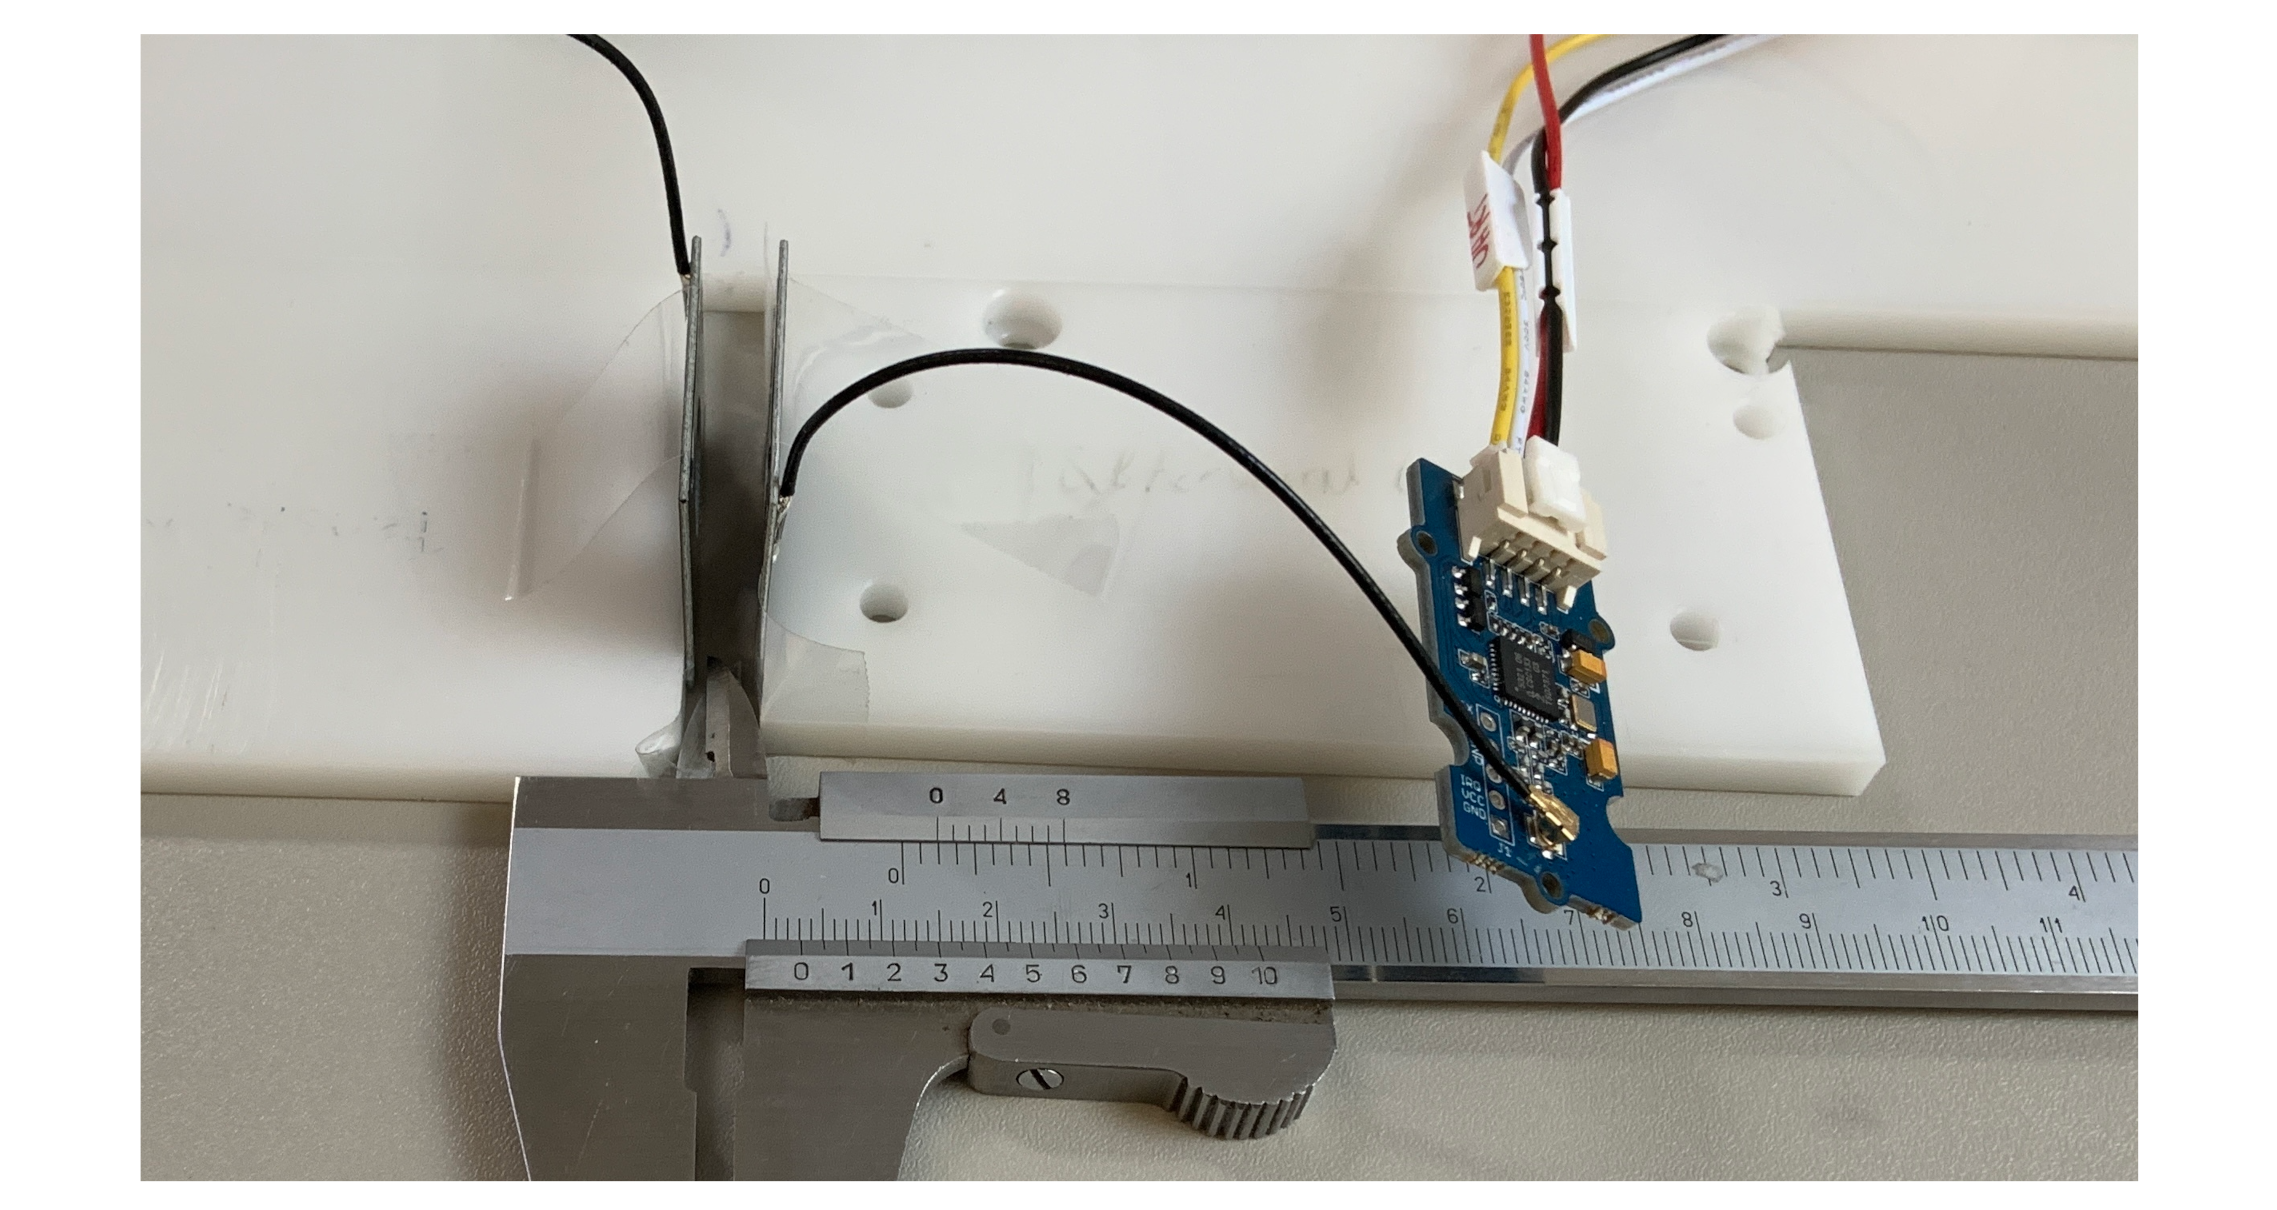
\includegraphics{images/ATC_nfc_range_test.png}
\caption{Grove PN532 NFC Reader mit Kabelgebundener Antenne
\label{ATC_nfc_range_test}}
\end{figure}

\begin{itemize}
\tightlist
\item
  test mit figuren nebeneinander
\end{itemize}

\hypertarget{schrittmotor-schrittmotorsteuerung}{%
\section{Schrittmotor /
Schrittmotorsteuerung}\label{schrittmotor-schrittmotorsteuerung}}

\begin{itemize}
\tightlist
\item
  warum =\textgreater{} einfache ansteuerung
\item
  keine STEP DIR somit muss embedded nicht echtzeitfähigsein und kann
  ggf auch andere task abbarbeiten
\item
  TMC schrittmotortreiber spi configuration
\item
  und goto move =\textgreater{} wait for move finished irw testen
\item
  dafür einfacher python testreiber geschribene
\item
  schrittverlust nicht zu erwarten
\end{itemize}

\hypertarget{d-druck-fuxfcr-den-mechanischen-aufbau}{%
\section{3D Druck für den mechanischen
Aufbau}\label{d-druck-fuxfcr-den-mechanischen-aufbau}}

Da es sich hier nur um einen Prototyp handelt, wurde hier auf ein
einfach zu verarbeitendes Filament vom Typ \gls{pla} zurückgegriffen.
Dieses ist besonders gut für die Prototypenendwicklung geeignet und kann
mit nahezu jeden handelsüblichen \gls{fdm} 3D-Drucker verarbeitet
werden.

Zuvor wurden einige Testdrucke durchgeführt, um die Qualität der zuvor
gewählten Druckparameter zu überprüfen und diese gegebenenfalls
anzupassen. Auch wurden verschiedene weitere Bauteile gedruckt, an
welchen die Toleranzen für die späteren \gls{cad} Zeichnungen
abgeschätzt werden können. Dies betrifft vor allem die Genauigkeit der
Bohrungen in den gefertigten Objekten, da hier später Bolzen und
Schrauben ein nahezu spielfrei eingeführt werden müssen. Ein Test,
welcher die Machbarkeit von Gewinden zeigt, wurde nicht durchgeführt, da
alle Schrauben später mit der passenden Mutter gesichert werden sollen.
So soll eine Abnutzung durch häufige Montage der gedruckten Bauteile
verhindert werden.

Bei dem Design der zu druckenden Bauteile wurde darauf geachtet, dass
diese den Bauraum von 200x200x200mm nicht überschreiten und somit auch
von einfachen \gls{fdm} 3D-Druckern erstellt werden können.

Als Software wurde der Open-Source Slicer Ultimaker Cura
\cite{ultimakercura} verwendet, da dieser zum einen bereits fertige
Konfigurationen für den verwendeten 3D-Drucker enthält und zum anderen
experimentelle Features bereitstellt.

\begin{figure}
\centering
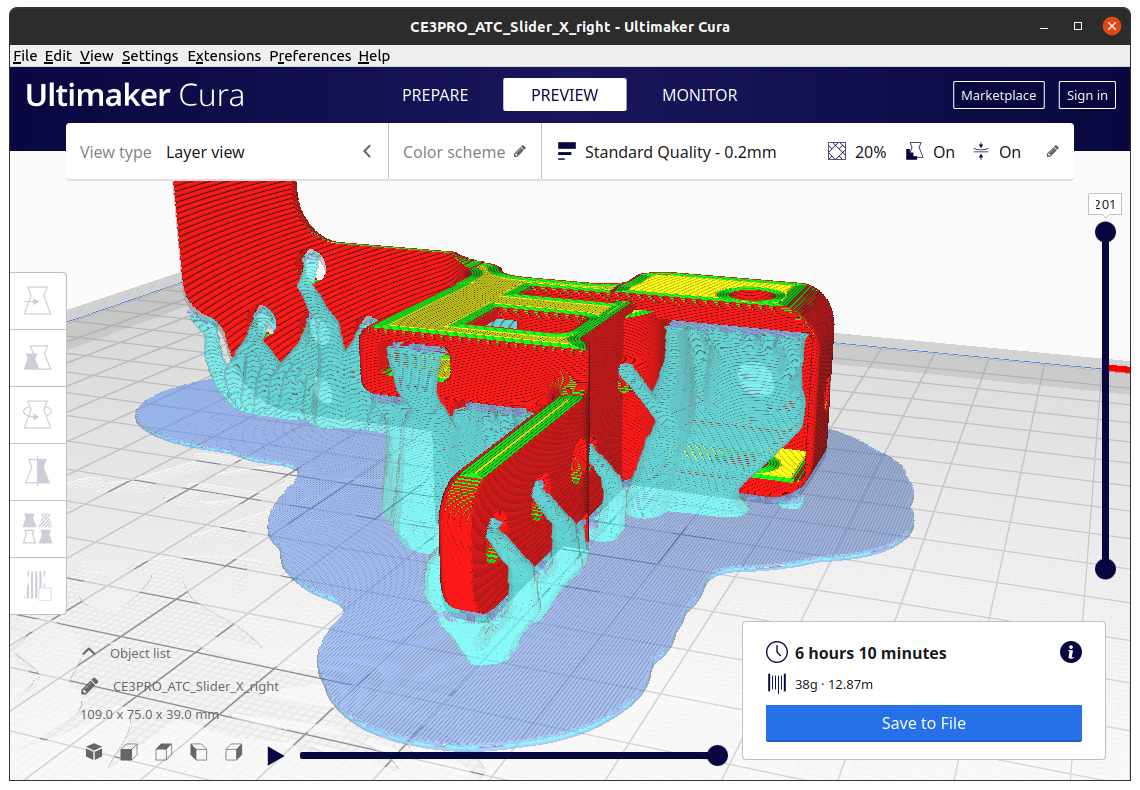
\includegraphics{images/3d_print_tree_structure.png}
\caption{3D Druck: Objekt (rot,gelb,grün),Tree Structure (cyan)
\label{3d_print_tree_structure}}
\end{figure}

Hier wurde für die Bauteile, welche eine Stützstruktur benötigen, die
von Cura bereitgestellte Tree Support Structure aktiviert.
\ref{3d_print_tree_structure} Diese bietet den Vorteil gegenüber anderen
Stützstrukturen, dass sich diese leichter entfernen lässt und weniger
Rückstände an den Bauteilen hinterlässt. Diese Vorteile wurde mit
verschiedenen Testdrucken verifiziert und kommen insbesondere bei
komplexen Bauteilen mit innenliegenden Elementen zum Tragen, bei denen
eine Stützstruktur erforderlich sind.

\begin{longtable}[]{@{}ll@{}}
\caption{Verwendete 3D Druck Parameter. Temperatur nach
Herstellerangaben des verwendeten PLA Filament.}\tabularnewline
\toprule
Ender 3 Pro 0.4mm Nozzle & PLA Settings\tabularnewline
\midrule
\endfirsthead
\toprule
Ender 3 Pro 0.4mm Nozzle & PLA Settings\tabularnewline
\midrule
\endhead
Layer Height & 0.2mm\tabularnewline
Infill & 50.00\%\tabularnewline
Wall Thickness & 2.0mm\tabularnewline
Support Structure & Tree\tabularnewline
Top Layers & 4\tabularnewline
Bottom Layers & 4\tabularnewline
\bottomrule
\end{longtable}

Zusätzliche Parameter wie die Druckgeschwindigkeit, sind hierbei
individuell für den zu gewählten 3D Drucker zu ermitteln. Allgemein
wurden hier die Standarteinstellungen verwendet, welche in diesem Falle
einen guten Kompromiss zwischen Qualität und Druckzeit lieferten.

\hypertarget{erstellung-erster-prototyp}{%
\chapter{Erstellung erster Prototyp}\label{erstellung-erster-prototyp}}

\begin{figure}
\centering
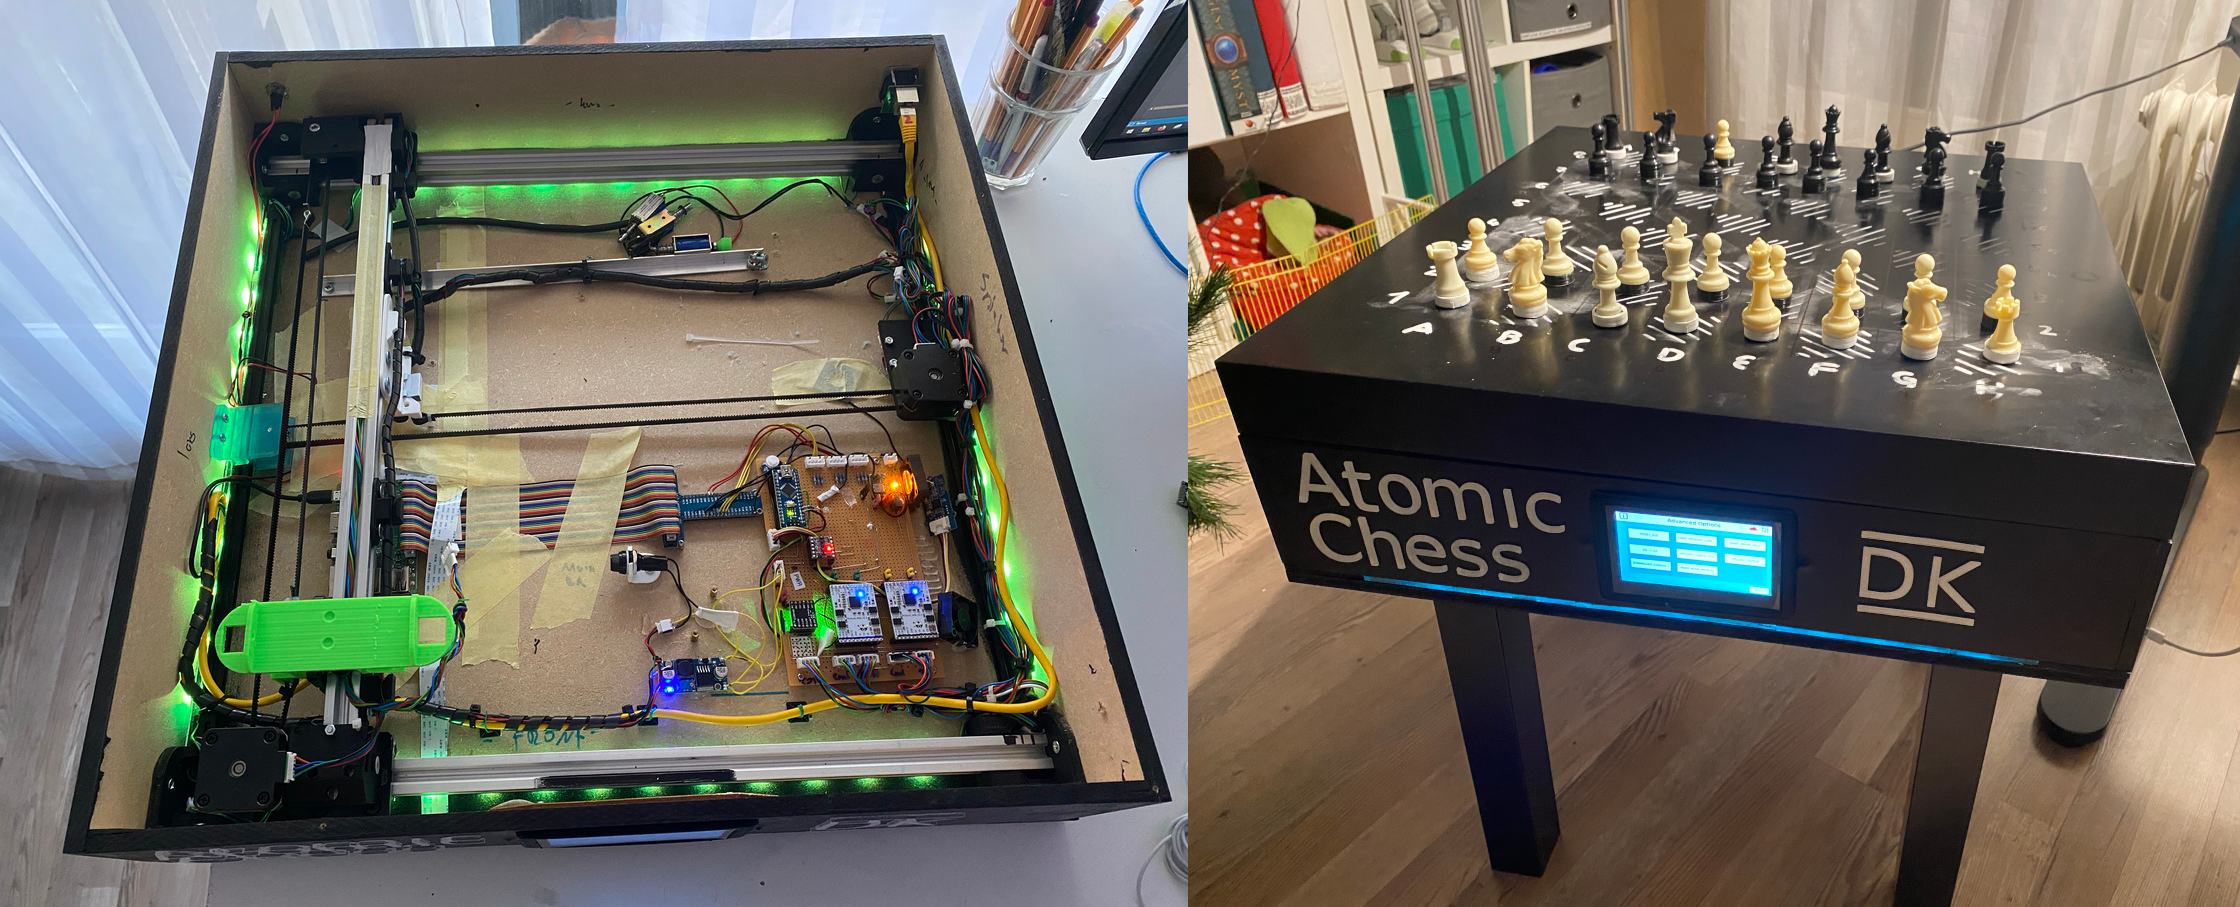
\includegraphics{images/table_images/dk.png}
\caption{Prototyp Hardware: Erster Prototyp des autonomen Schachtisch
\label{dk}}
\end{figure}

\hypertarget{mechanik}{%
\section{Mechanik}\label{mechanik}}

Bei dem mechanischen Aufbau wurde auf ein einfaches Design geachtet. Die
Konstruktion wurde im Vorfeld in einem \gls{cad} Programm durchgeführt
und die Grundkonstruktion in mehreren Iterationsschritten verfeinert.
Das verwendete \gls{cad} Programm `Autodesk Fusion 360' bietet, eine
einfache Umsetzung auch für Personen, welche keine Ausbildung im Bereich
der Mechanik und Entiwcklung vorweisen können.

Bei der initialen Planung wurde beachtet, einen möglichst kleinen
Fußabdruck des Schachtischs zu realisieren. Darüberhinaus wurde
beabsichtigt, eine fertige Schachtischplatte als Basis zu verwenden und
die Mechanik unter diese zu konstruieren. Um dies zu ermöglichen wurde
ein IKEA Lack Tisch verwendet, welcher die Idealen Abmessungen von
55x55cm hat und somit eine erforderliche Schachfeldgröße von 55mm
möglich ist. Durch den bereits vorhandenen Rahmen ist es simpel möglich,
weitere Komponenten an diesem zu befestigen. Somit stellt diese
Tischplatte eine ideale Basis für den autonomen Schachtisch dar.

Für die Achsenführung der beiden X- und Y-Achsen wurden konventionelle
20x20mm Aluminium-Profile verwendet, welche mit einfachen Mitteln und
wenig Geschick passend zugeschnitten werden können. Allgemein wurde eine
X-Y Riemenführung verwendet, wobei jede Achse einen separaten Nema 17
Schrittmotor inklusive des passenden Endschalters montiert hatte. Bei
den Schlitten, welche auf den Aluminium-Profilen laufen, wurden fertige
Standartkomponenten verwendet, um das Spiel in der Mechanik zu
minimieren. Diese stellen jedoch einen großen Posten in der
Preiskalkulation dar. Die Vortiele überwogen jedoch, da diese nicht
manuell erstellt und getestet werden müssen.

Bereits während des Designprozess konnte anhand einer statischen
Simulation des Modells erkannt werden, dass trotz der Optimierung des
Fahrweges beider Achsen durch die Verkleinerung der Halterungen der
Aluminium-Profile dieser nicht ausreicht. Mit dieser Konstellation
können die Figuren nicht ausreichend weit aus dem Spielfeld platziert
werden und verbleiben in den äußeren Spielfeldern. Dieser Effekt war
unerwünscht und schränkt das Spielerlebnis deutlich ein.

Um dies zu verhindern wurde der zentrale Schlitten der Y-Achse, auf
welchem der Elektromagnet für die Figur-Mitnahme platziert ist, um einen
weiteren Elektromagnet erweitert. Diese befinden sich nun nicht mehr
mittig auf dem Schlitten, sondern wurden um 110mm in Richtung der
X-Achse versetzt. So ist es möglich Figuren bis ganz an den Rand
verschieben zu können.

Diese Lösung erfordert jedoch einen komplexeren
Bahnplanungs-Algorithmus, da die Elektromagneten zwischen einzelnen
Zügen gewechselt werden müssen. Dies führt zu einem zeitlich kürzeren
Stillstand der Figur auf dem Schachfeld.

Alle selbst-konstruierten Teile wurden anschließend mittels 3D Druck
erstellt und konnten in die Tischplattenbasis eingeschraubt werden. Die
Verwendung der aus Holz bestehenden Grundplatte erschwerte jedoch eine
akkurate Platzierung der Teile und die bereits existierenden Seitenwände
schränkten diese noch zusätzlich ein. Somit erforderte der komplette
Zusammenbau mehrere Tage und zusätzliche Iterationen des 3D-Designs, um
den Einbau spezifischer Teile zu ermöglichen. Das Design stellt jedoch
eine solide Grundlage darf, welche für die weitere Software und
Hardware-Entwicklung essentiell ist.

\hypertarget{parametrisierung-schachfiguren}{%
\section{Parametrisierung
Schachfiguren}\label{parametrisierung-schachfiguren}}

Da das System die auf dem Feld befindlichen Schachfiguren anhand von
\gls{nfc} Tags erkennt, müssen diese zuerst mit Daten beschrieben
werden. Die verwendeten NXP NTAG 21 Chips, besitzen einen vom Benutzer
verwendbaren Speicher von 180 Byte. Dieser kann über ein
\gls{nfc}-Lese/Schreibger mit Daten verschiedenster Art beschrieben und
wieder ausgelesen werden. Moderne Mobiltelefone besitzen in der Regel
auch die Fähigkeit mit passenden \gls{nfc} Tags kommunizieren zu können;
somit sind keine Stand-Alone Lesegeräte mehr notwendig.

Der Schachtisch verwendet dabei das \gls{ndef} Dateiformat welches
Festlegt, wie die Daten auf dem \gls{nfc} Tag gespeichert werden. Da
diesen ein Standardisiertes Format ist, können alle gängigen Lesegeräte
und Chipsätze diese Datensätze lesen. Der im autonomen Schachtisch
verwendete Chipsatz PN532 von NXP ist dazu ebenfalls in der Lage.

Um das \gls{ndef} Format verwenden zu können, müssen die \gls{nfc} Tags
zuerst auf diese formatiert werden. Die meisten käuflichen Tags sind
bereits derart formatiert. Alternativ kann dies mittels Mobiltelefons
und passender Applikation geschehen. Da \gls{ndef} Informationen über
die Formatierung und der gespeicherten Einträge speichert, stehen nach
der Formatierung nur noch 137 Bytes des NXP NTAG 21 zur Verfügung.

Per Lesegerät können anschließend mehrere \gls{ndef} Records auf den Tag
geschrieben werden. Diese sind mit Dateien auf einer Festplatte
vergleichbar und können verschiedenen Dateiformate und Dateigrößen
annehmen. Ein typischer Anwendungsfall ist der \gls{ndefrtd} URL
Datensatz. Dieser kann dazu genutzt werden eine spezifizierte URL auf
dem Endgeräte aufzurufen, nachdem der \gls{nfc} Tag gescannt wurde.
\cite{nordicnfclibndef}

Der autonome Schachtisch verwendet den einfachsten \gls{ndefrtd} Typ,
den sogenannten Text-Record, welcher zum Speichern von Zeichenketten
genutzt werden kann, ohne das eine Aktion auf dem Endgerät ausgeführt
wird. Jeder Tag einer Schachfigur, welche für den autonomen Schachtisch
verwendet werden kann, besitzt diesen \gls{ndef} Record an der ersten
Speicher-Position. Alle weiteren eventuell vorhandenen Records werden
vom Tisch ignoriert. \cite{nordicnfclib}

\begin{figure}
\centering
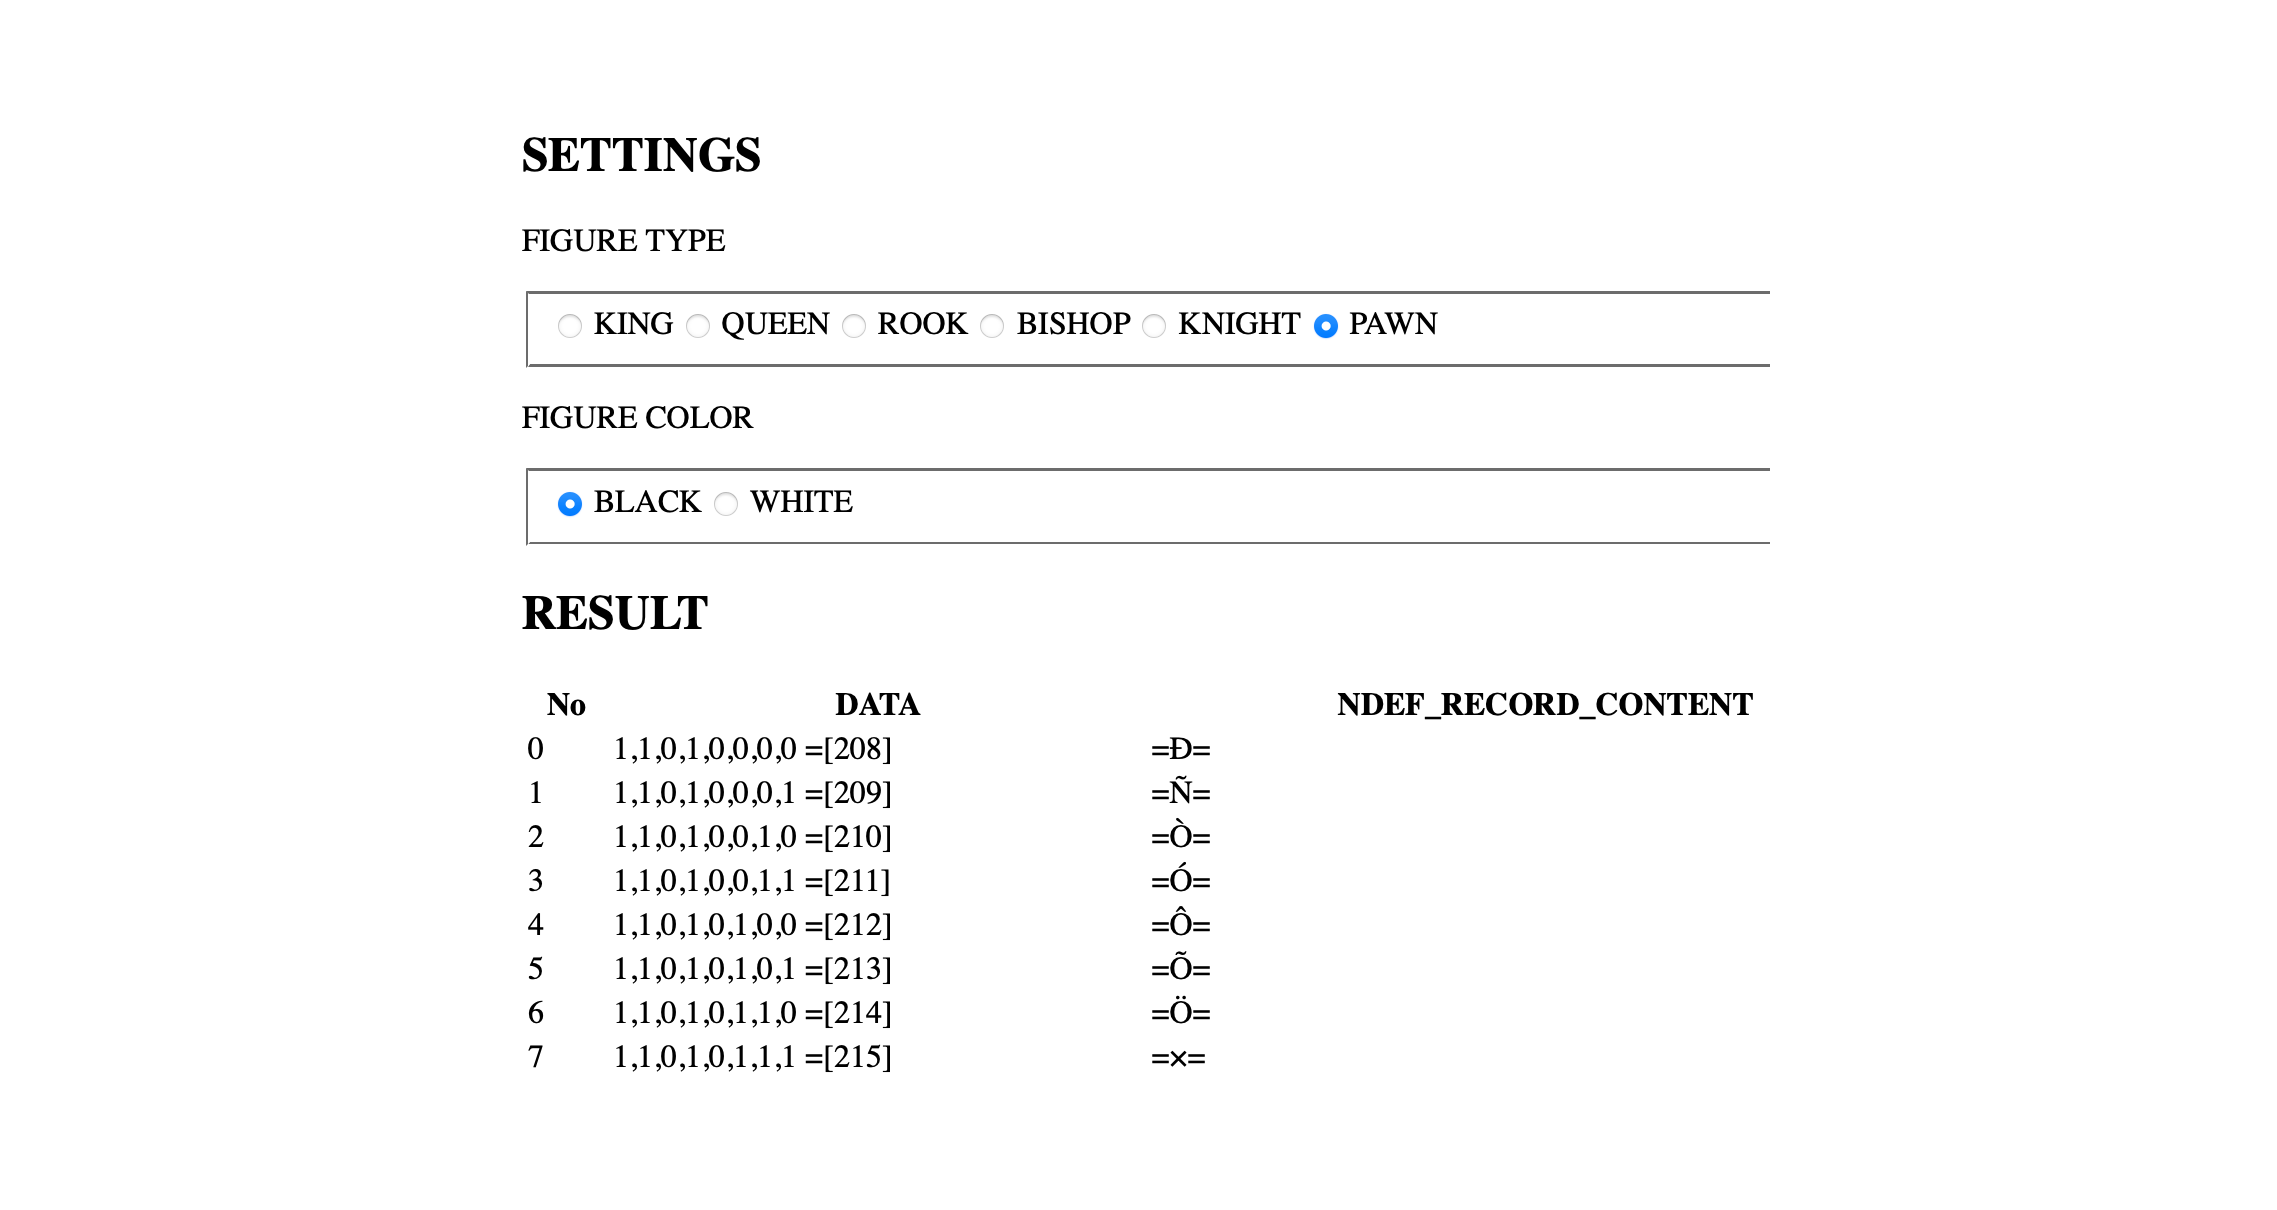
\includegraphics{images/ATC_ChessFigureIDGenerator.png}
\caption{Prototyp Hardware: Tool zur Erstellung des NDEF Payloads:
ChessFigureIDGenerator.html \label{ATC_ChessFigureIDGenerator}}
\end{figure}

Um die Payload für den \gls{nfc} Record zu erstellen wurde ein kleine
Web-Applikation erstellt, welche den Inhalt der Text-Records erstellt.
Dieser ist für jede Figur individuell und enthält den Figur-Typ und die
Figur-Farbe. Das Tool unterstützt auch das Speichern weiterer Attribute
wie einem Figur-Index, welcher aber in der finalen Software-Version
nicht genutzt wird. \ref{ATC_ChessFigureIDGenerator}

Nach dem Beschreiben eines \gls{nfc} Tags ist es zusätzlich möglich,
diesen gegen Auslesen mittels einer Read/Write-Protection zu schützen.
Diese Funktionalität wird jedoch nicht verwendet, um das Kopieren
einzelner Figuren durch den Benutzer zu ermöglichen. Somit kann dieser
leicht seine eigenen Figuren erschaffen, ohne auf das Tool angewiesen zu
sein. Auch ist es so möglich, verschiedene Figur-Sets zu mischen; somit
kann ein Spieler verschiedene Sets an Figuren mit dem autonomen
Schachtisch verwenden.

\begin{figure}
\centering
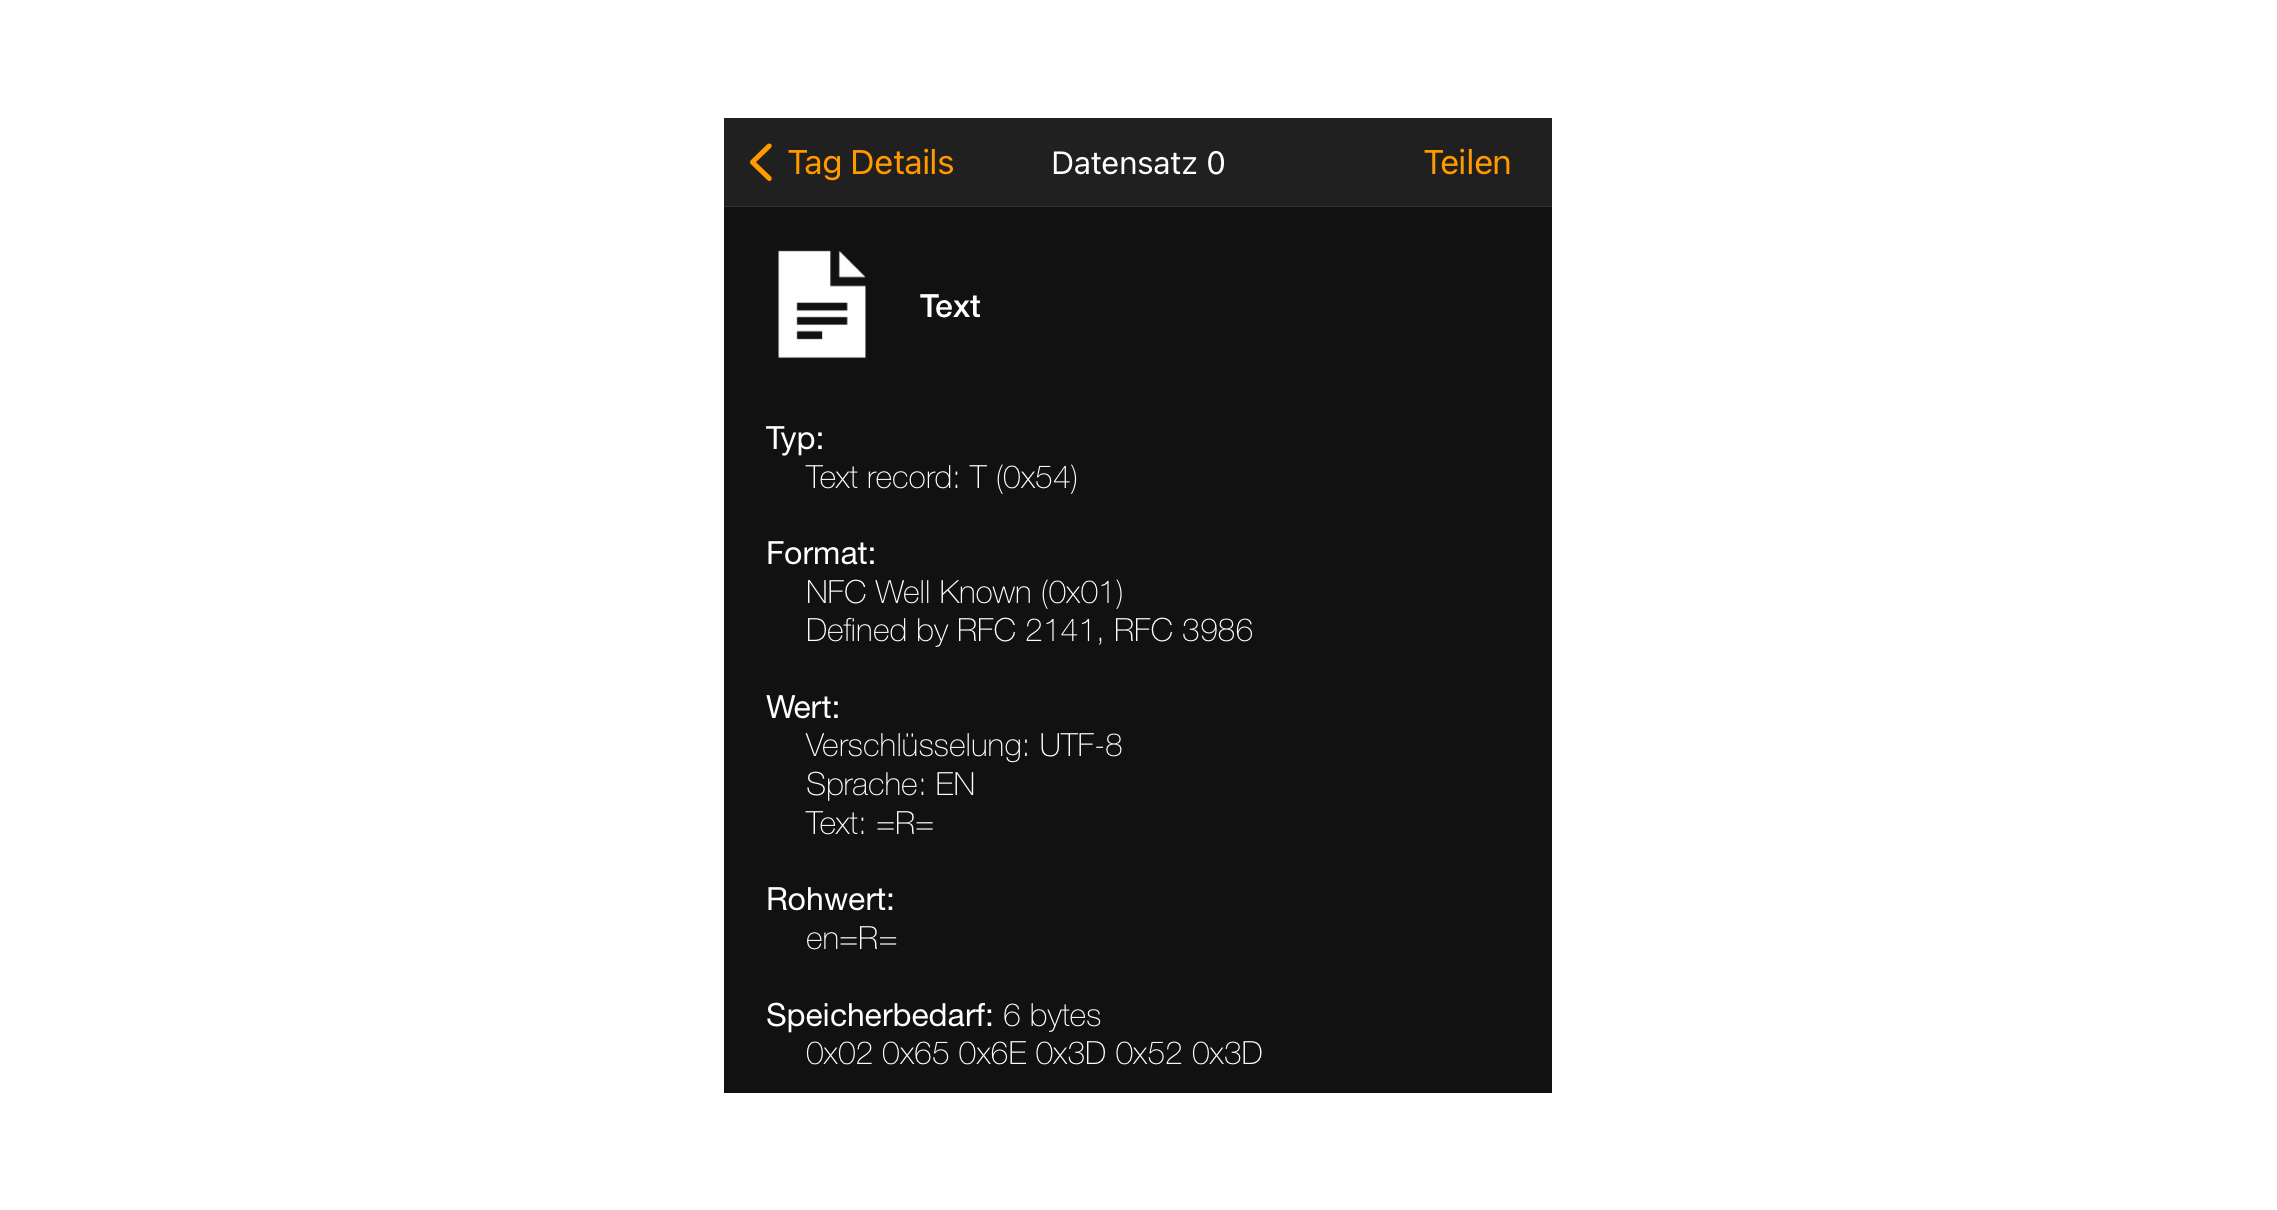
\includegraphics{images/ndef_record_rook.png}
\caption{Prototyp Hardware: NDEF Text Record Payload für einen weißen
Turm \label{ndef_record_rook}}
\end{figure}

\hypertarget{schaltungsentwurf}{%
\section{Schaltungsentwurf}\label{schaltungsentwurf}}

\begin{figure}
\centering
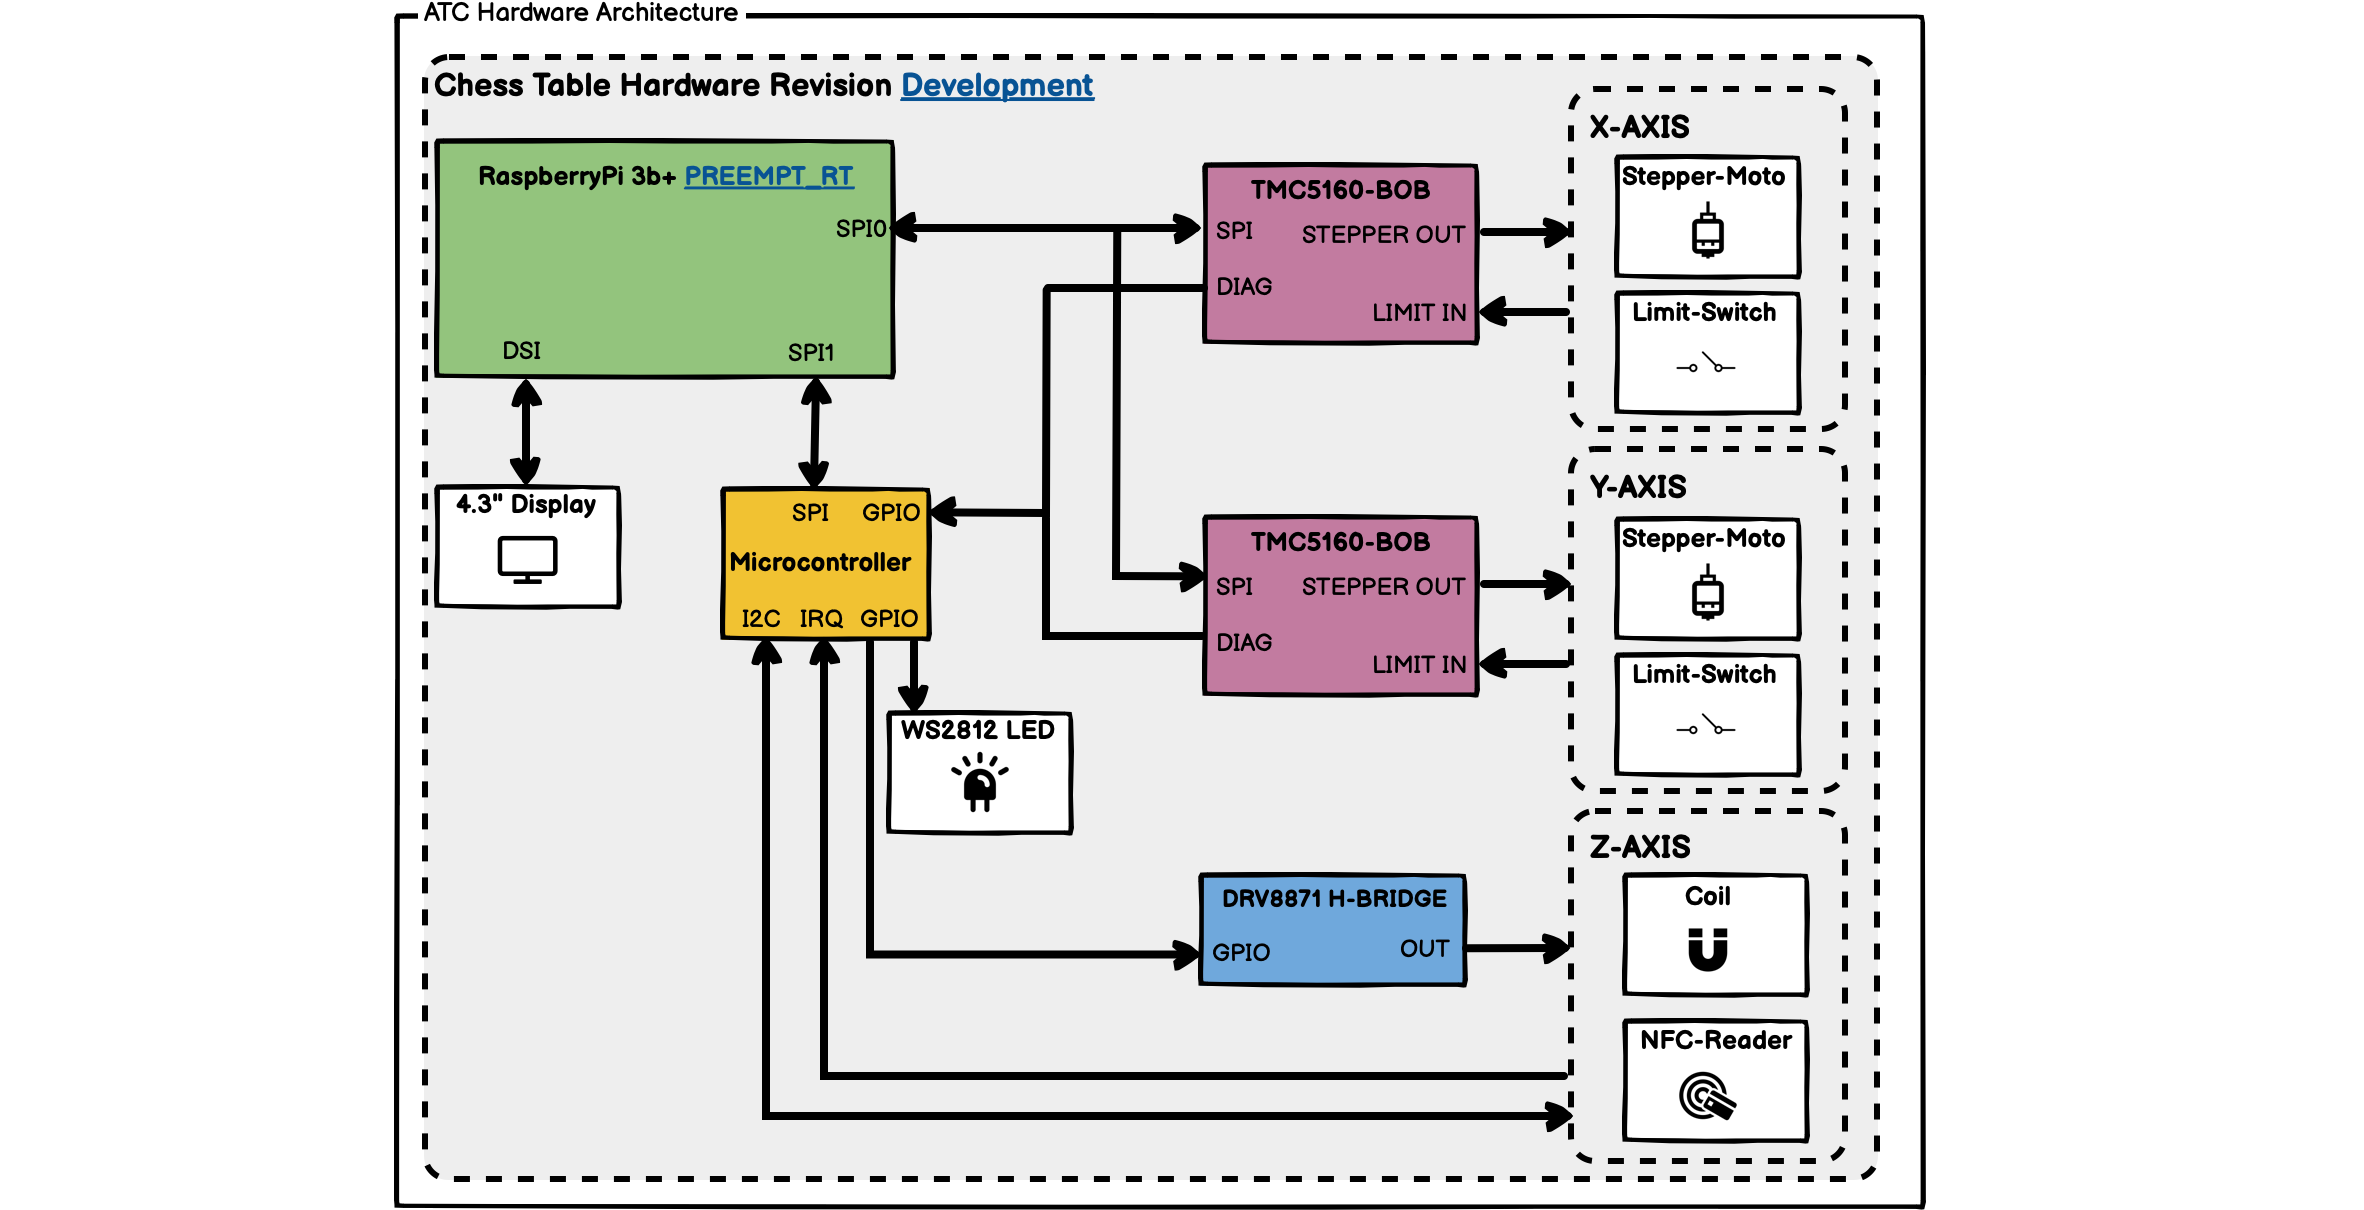
\includegraphics{images/ATC_Hardware_Architecture_DK.png}
\caption{Prototyp Hardware: Blockdiagramm
\label{ATC_Hardware_Architecture_DK}}
\end{figure}

\begin{itemize}
\tightlist
\item
  auswahl der Motortreiber (leise, bus ansteuerung)
\item
  ansteuerung pn532 und umsetzung auf uart
\end{itemize}

\begin{figure}
\centering
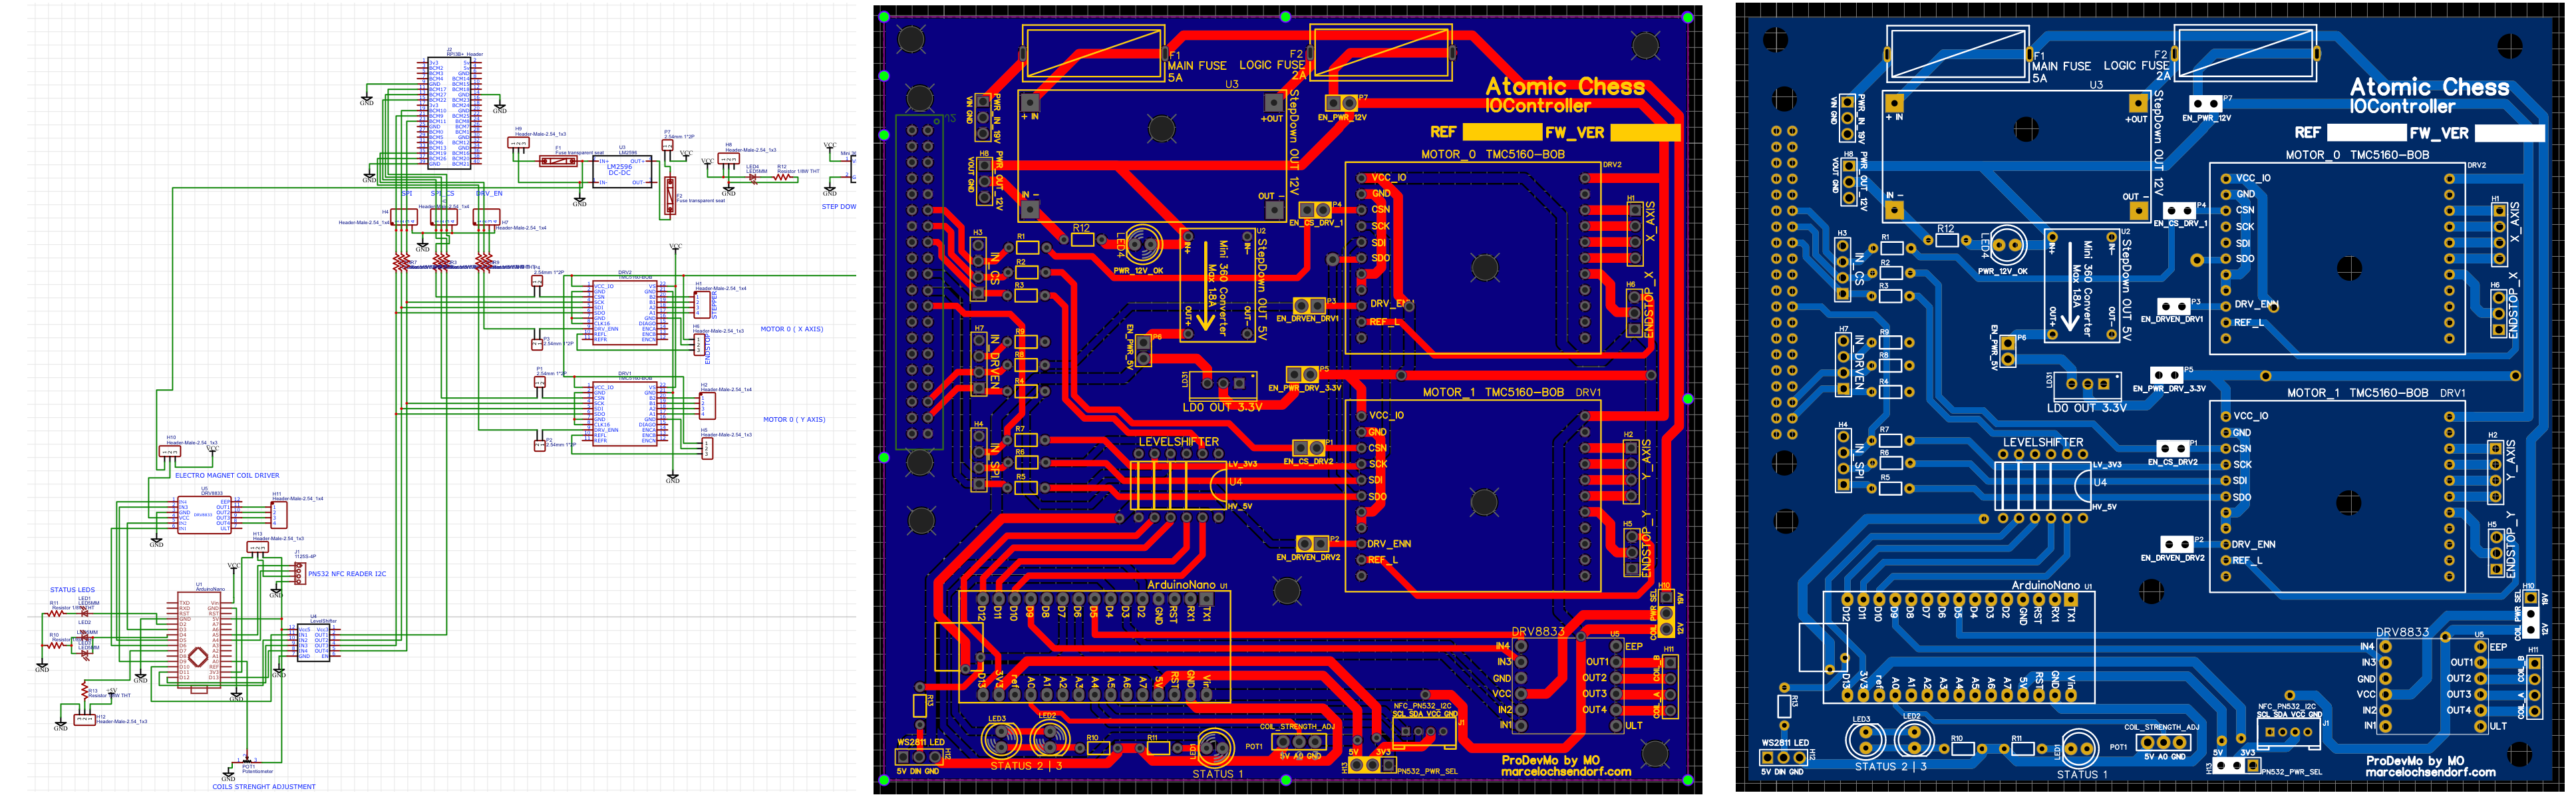
\includegraphics{images/ATC_DK_HW_SCHEM.png}
\caption{Prototyp Hardware: Schaltplan und finaler PCB Entwurf
\label{ATC_Schematic_DK}}
\end{figure}

\begin{itemize}
\tightlist
\item
  platinendesign
\item
  ansterung elektromagnetet
\end{itemize}

\hypertarget{implementierung-hal}{%
\subsection{Implementierung HAL}\label{implementierung-hal}}

\begin{itemize}
\item
  ansteuerung des TMC5160
\item
  ansterung des Microncontollers (PN532, LED)
\item
  integration in controller software
\item
  welche funktion stehen bereit tabelle
\item
  step dir interface =\textgreater{} erfodert jedoch eine rt fähige \#\#
  Fazit bezüglich des ersten Prototypens
\item
  nicht für production geeignet
\item
  aufbau und calibrierung langwiehrig
\item
  trotzdem robustes design auf kleinem formfaktor
\item
  verwendeten elektromagnete nicht stark genug, somit über aqusserhalb
  der specs betrieben was zu temeraturproblemen führte
\item
  gewicht der Figuren zu klein bzw magnete zu start
\item
  workarounds in der software nötig durch die beiden magnete
\item
  nicht die beste entscheidung direkt auf grösse zu optimieren
\end{itemize}

\hypertarget{erstellung-des-zweiter-prototypens}{%
\chapter{Erstellung des zweiter
Prototypens}\label{erstellung-des-zweiter-prototypens}}

\begin{figure}
\centering
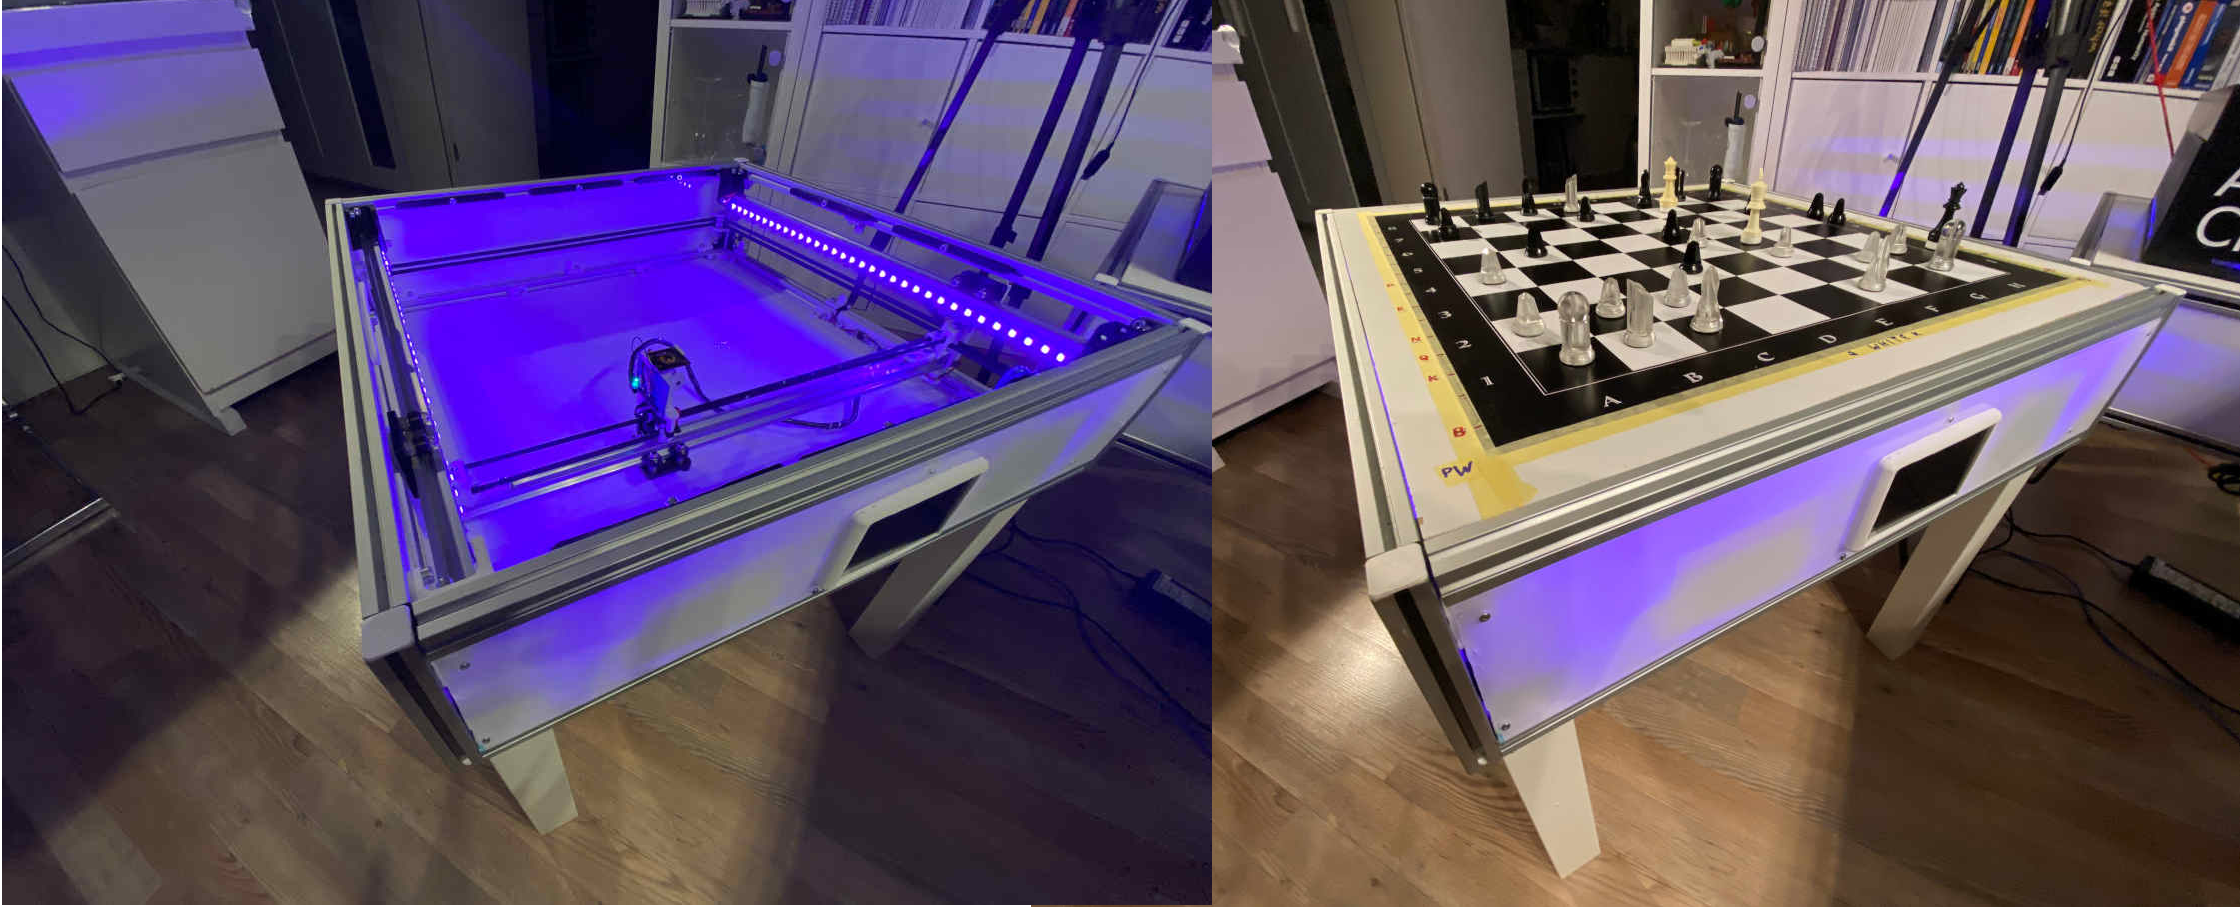
\includegraphics{images/table_images/prod.png}
\caption{Producation Hardware: Finaler autonomer Schachtisch
\label{prod}}
\end{figure}

\hypertarget{modifikation-der-mechanik}{%
\section{Modifikation der Mechanik}\label{modifikation-der-mechanik}}

\begin{itemize}
\tightlist
\item
  Dauertest hat gezeigt dass Mechanik zu viel spiel aufweisst
\item
  Motorenhalterung der y achse schränkt des bewegungsspielraum um mehr
  als 10cm ein, welches zu einem unwesentlichen grösseren verhältnis von
  Spielfeldgrösse und Abmessungen des Schachtischs
\item
  CoreXY bietet Vorteil:
\item
  Motoren fest am rahmen =\textgreater{} weniger kabel + gewicht an der
  Y Achse
\item
  jedoch komplexerer Aufwand der riemenverlegung so komplexere 3d
  bauteile
\item
  Tischabmessungen 620x620mm dabei Bewegungsspielraum vom 580x580 zuvor
  nur 480x480
\item
  langer zusammenbau !!
\end{itemize}

\hypertarget{optimierungen-der-spielfiguren}{%
\section{Optimierungen der
Spielfiguren}\label{optimierungen-der-spielfiguren}}

Die bisherigen genutzten vorgefertigten Figuren funktionierten mit dem
ersten Prototyp ohne erkennbare Fehler. Sie wiesen aber trotzdem eine zu
hohe Fehleranfälligkeit, in Bezug auf das gegenseitige Beeinflussen
(abstoßen, anziehen) durch die verwendeten Magnete auf.

Die Größe der Figuren kann durch die fest definierte Schachfeldgröße von
55mm und der verwendeten \gls{nfc} Tags nicht verändert werden. Nach
einigen Testdurchläufen mit dem ersten Prototyp war zu erkennen, dass
sich die Figuren je nach aktueller Situation auf dem Spielfeld weiterhin
magnetisch anziehen. Um diesen Fehler zu beheben wurden verschiedenen
Bewegungsgeschwindigkeiten getestet, ergaben allerdings für diesen
Anwendungsfall keine merkliche Verbesserung.

Dies führt je nach Spielverlauf zu Komplikationen, sodass die Figuren
manuell vom Benutzer wieder mittig auf den Felder platziert werden
müssen.

Um dies zu verhindern, wurde einige Figuren zusätzlich mit einer 20mm
Unterlegscheibe am Boden beschwert. Diese behob das Problem, jedoch
erwies sich das \gls{nfc} Tag nicht mehr als lesbar. Dies resultierten
aus dem Prozessgedanken, die Schachfiguren ebenfalls selbst mit dem
3D-Drucker herzustellen und die Magnete direkt in den Boden der Figur
einlassen zu können.

Die aktuell verwendeten Figuren des ersten Protoyp wiegen zwischen 8
Gramm für die Bauern und 10 Gramm für die restlichen Figuren. Der Test
mit der Unterlegscheibe ergab das diese mit 5 Gramm zusätzlich genug
Gewicht hinzufügen, um die magnetische Beeinflussung zu unterbinden.

Testweise wurden einige Figuren mittels 3D Drucker erstellt, um so das
Gewicht zu erhöhen. Nach einem erfolgreichen Test wurde das \gls{cad}
Modell so angepasst, dass sich der Magnet direkt in den Boden der Figur
einkleben lässt. Des Weiteren wurden bei den Bauern die Magnete
ausgetauscht. Die zuerst verwendeten 10x3mm Neodym-Magnete wurden bei
diesen Figuren gegen 6x3mm Magnete getauscht. Somit sind im Design zwei
verschiedenen Arten von Magneten notwendig, jedoch traten in den
anschließend durchgeführten Testläufen keine Beeinflussungen mehr auf.

\hypertarget{uxe4nderungen-der-elektronik}{%
\section{Änderungen der Elektronik}\label{uxe4nderungen-der-elektronik}}

Mit ein relevanter Kritikpunkt, welcher bereits während des Aufbaus des
ersten Prototyps zu erkennen war, ist die Umsetzung der Elektronik.
Diese wurde im ersten Prototyp manuell aufgebaut und enthielt viele
verschiedene Komponenten.

Die verwendeten Motortreiber stellten sich während der Entwicklung als
sehr flexibel heraus, stellten aber auch einen signifikanten
Kostenfaktor dar. Nach dem Aufbau und Erprobung des ersten Prototyps
wurde ersichtlich, dass hier nicht alle zuerst angedachten Features der
Treiber benötigt werden und so auch Alternativen in Betracht gezogen
werden konnten. Zusätzlich konnte die Elektronik nur beschränkt mit
anderen Systemen verbunden werden, was insbesondere durch die verwendete
\gls{spi} Schnittstelle geschuldet war.

All diese Faktoren erschweren einen einfachen Zusammenbau des autonomen
Schachtischs. Die Lösung stellt die Verwendung von Standardhardware dar.
Nach der Minimierung der elektrischen Komponenten und des mechanischen
Aufbaus ist zu erkennen, dass der autonome Schachtisch einer CNC-Fräse
bzw. eines 3D Drucker stark ähnelt. Insbesondere die XY-Achsen Mechanik
sowie die Ansteuerung von Schrittmotoren wird in diesen Systemen
verwendet. Mit dem Durchbruch von 3D Druckern im Konsumer-Bereich sind
auch kleine und preisgünstige Steuerungen erhältlich, welche 2-3
Schrittmotoren und diverse zusätzliche Hardware ansteuern können.

\begin{longtable}[]{@{}llll@{}}
\caption{Standardhardware 3D Drucker Steuerungen}\tabularnewline
\toprule
& SKR 1.4 Turbo & Ramps 1.4 & Anet A8 Mainboard\tabularnewline
\midrule
\endfirsthead
\toprule
& SKR 1.4 Turbo & Ramps 1.4 & Anet A8 Mainboard\tabularnewline
\midrule
\endhead
Stepper Driver & TMC2209 & A4988 / TMC2209 & A4988\tabularnewline
LED Strip Port & WS2811 / RGB & - & -\tabularnewline
Firmware & Marlin-FW 2.0 & Marlin-FW 1.0 & Proprietary\tabularnewline
\bottomrule
\end{longtable}

Hierbei existiert eine große Auswahl dieser mit den verschiedensten
Ausstattungen. Bei der Auswahl dieser wurde vor allem auf die
Möglichkeit geachtet sogenannte Silent-Schrittmotortreiber verwenden zu
können, um die Geräuschimmissionen durch die Motoren so weit wie möglich
zu minimieren. Im ersten Prototyp wurde unter anderem aus diesem Grund
die TMC5160-BOB Treiber ausgewählt. Hierzu wurde der
Schrittmotor-Treiber TMC2209 gewählt, welcher diese Features ebenfalls
unterstützt und in der Variante als Silent-Step-Stick direkt in die
meisten 3D Drucker Steuerungen eingesetzt werden können. Hierbei ist es
wichtig, dass auf der gewählten Steuerung die Treiber-ICs nicht fest
verlötet sind, sondern getauscht werden können. Ein weiterer Punkt ist
die Kommunikation der Steuerung mit dem Host-System. Hierbei setzten
alle untersuchten Steuerungen auf die \gls{usb} Schnittstelle und somit
ist eine einfache Kommunikation gewährleistet. Das verwendete
eingebettete System im autonomen Schachtisch bietet vier freie \gls{usb}
Anschlüsse, somit ist eine einfache Integration gewährleistet.

\begin{figure}
\centering
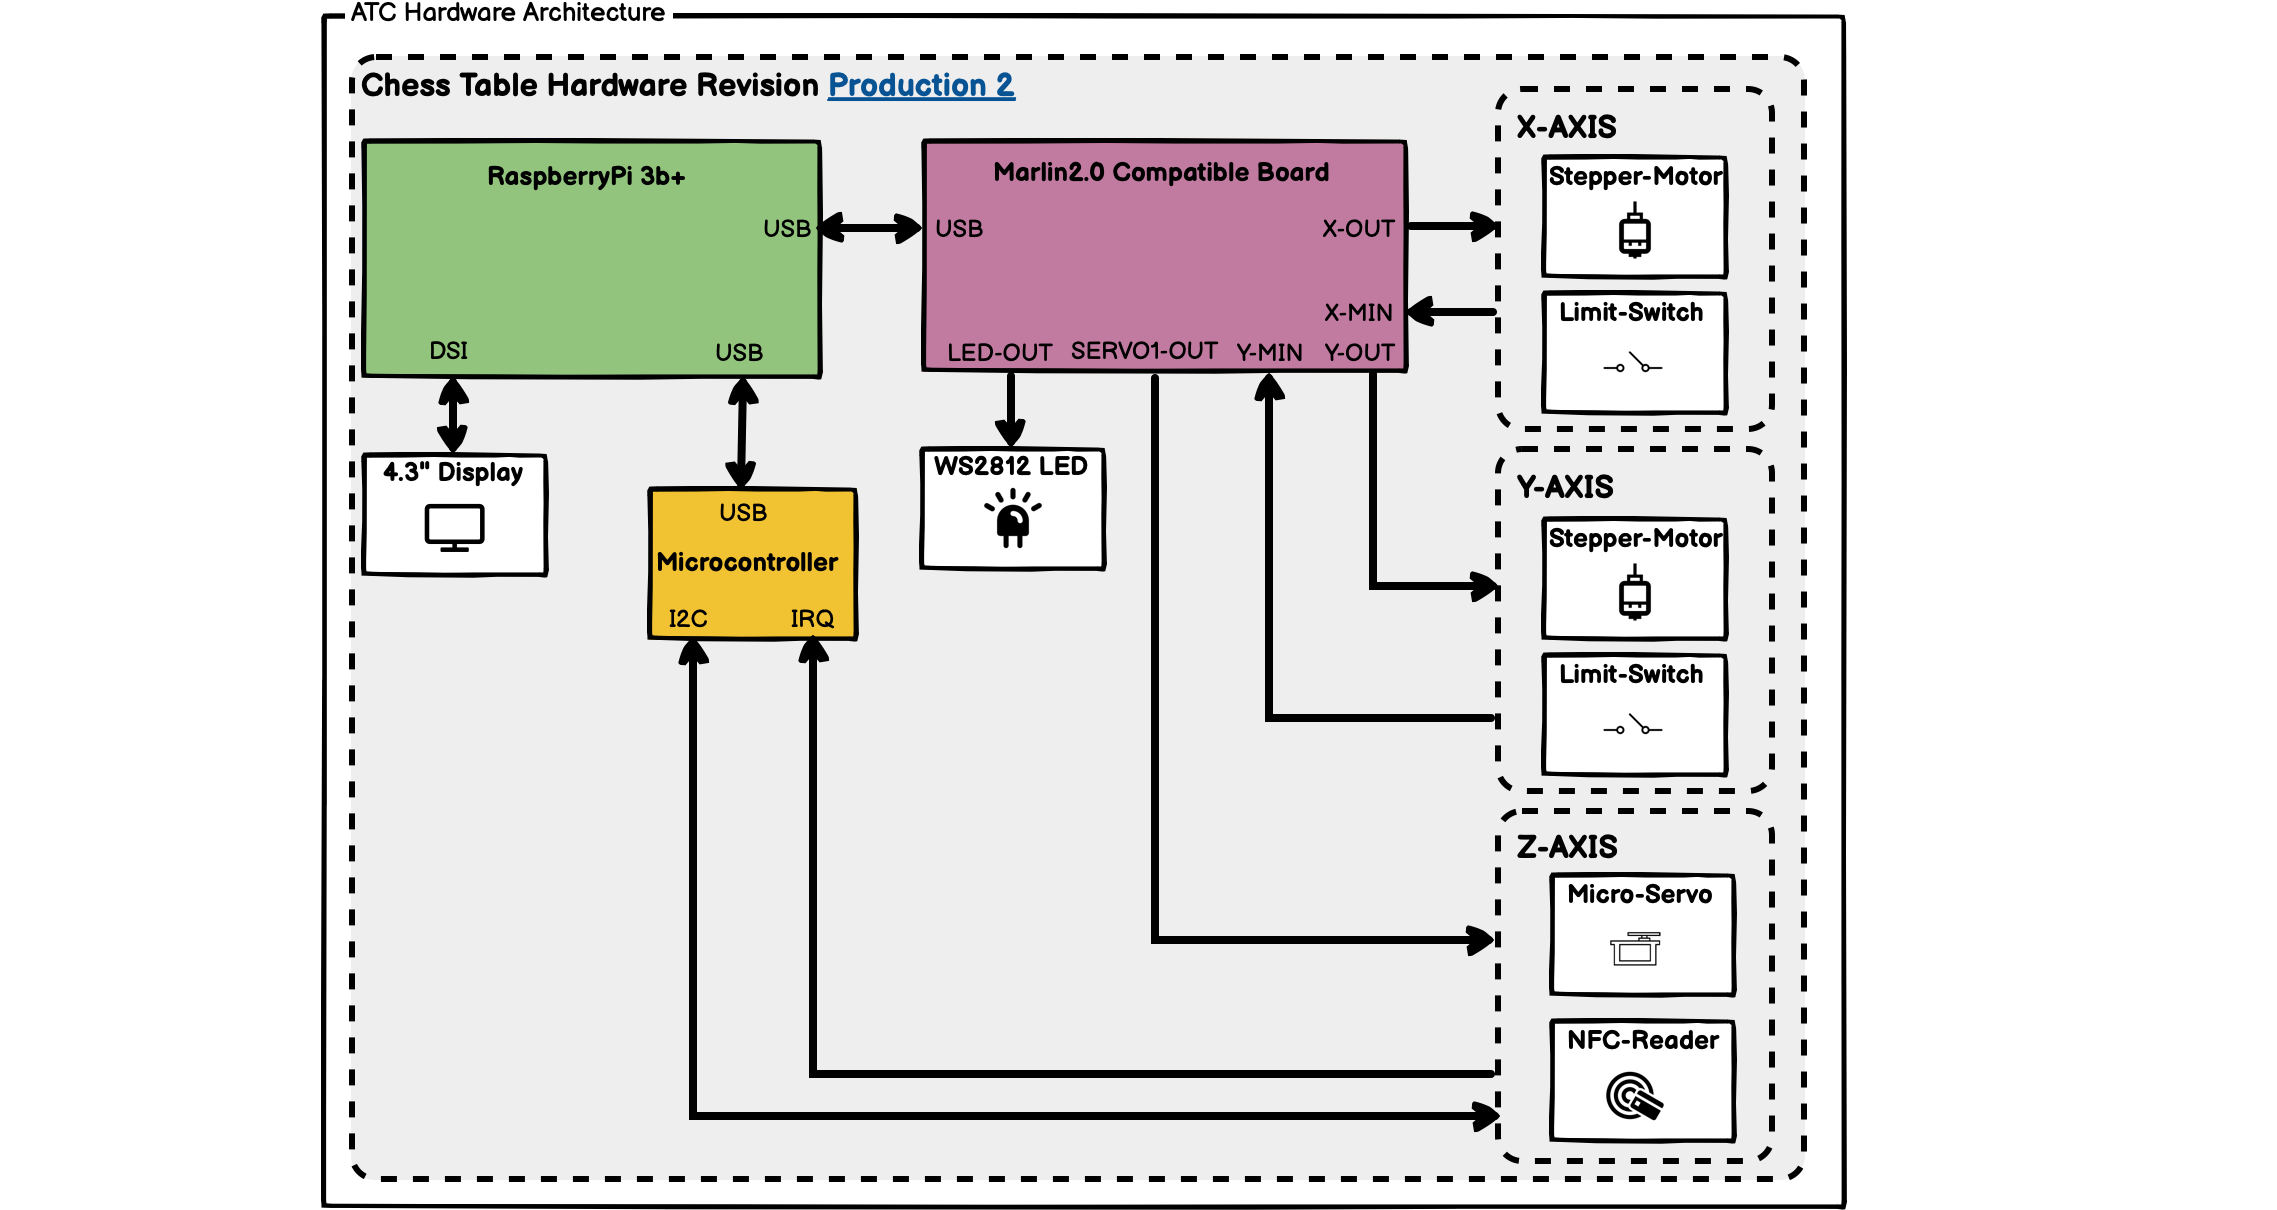
\includegraphics{images/ATC_Hardware_Architecture_PROD.png}
\caption{Producation Hardware: Blockdiagramm
\label{ATC_Hardware_Architecture_PROD}}
\end{figure}

Nach einer gründlichen Evaluation der zur Verfügung stehenden
Steuerungen, wurde die SKR 1.4 Turbo Steuerung ausgewählt, da diese
trotz des geringfügig höheren Marktpreises genug Ressourcen auch für
spätere Erweiterung bietet und eine Unterstützung für die neuste Version
der Marlin-FW\cite{marlinfw} bereitstellt. Somit wurde die
Elektronik durch die verwendete Plug\&Play stark vereinfacht
\ref{ATC_Hardware_Architecture_PROD}.

\hypertarget{hal-implementierung-gcode-sender}{%
\subsection{HAL: Implementierung
GCODE-Sender}\label{hal-implementierung-gcode-sender}}

Durch die durchgeführten Änderungen an der Elektronik insbesondere durch
die Verwendung einer Marlin-FW\cite{marlinfw} fähigen
Motorsteuerung, ist eine Anpassung der \gls{hal} notwendig. Diese
unterstütz die Ansteuerung der Motoren und anderen Komponenten (z.B.
Spindeln, Heizelemente) mittels G-Code und wird typischerweise in 3D
Druckern und CNC-Fräsen eingesetzt. G-Code ist eine
Marlin-FW\cite{marlinfw} biete dabei einen großen Befehlssatz an
G-Code Kommandos an. Bei diesem Projekt werden jedoch nur einige G-Code
Kommandos verwendet, welche sich insbesondere auf die Ansteuerung der
Motoren beschränken.

\begin{longtable}[]{@{}lll@{}}
\caption{Grundlegende verwendete G-Code Kommandos}\tabularnewline
\toprule
& G-Code Command & Parameters\tabularnewline
\midrule
\endfirsthead
\toprule
& G-Code Command & Parameters\tabularnewline
\midrule
\endhead
Move X Y & G0 & X Y\tabularnewline
Move Home Position & G28 & -\tabularnewline
Set Units to Millimeters & G21 & -\tabularnewline
Set Servo Position & M280 & P S\tabularnewline
Disable Motors & M84 & X Y\tabularnewline
\bottomrule
\end{longtable}

Die erforderlichen Kommandos wurden auf ein Minimum beschränk, um eine
maximale Kompatibilität bei verschiedenen G-Code-fähigen Steuerungen zu
gewährleisten. Die Software unterstützt jedoch weitere Kommandos wie
z.B. \passthrough{\lstinline!M150!} mit welche speziellen Ausgänge für
LEDs gesteuert werden können. Dieses Feature bietet sowohl die
verwendete Marlin-FW\cite{marlinfw} als auch die verwendete
Steuerung an. Sollte die verwendete Steuerung solch ein optionales
Kommando nicht unterstützen, so werden diese ignoriert was zur Folge
hat, dass auch preisgünstige Steuerungen verwendet werden können.

Die Kommunikation zwischen Steuerung und eingebetteten System geschieht
durch eine \gls{usb} Verbinden. Die Steuerung meldet sich als virtuelle
Serielle Schnittstelle im System an und kann über diese mit der Software
kommunizieren. Auch werden so keine speziellen Treiber benötigt, da auf
nahezu jedem System ein Treiber (USB-CDC) für die gängigsten \gls{usb}
zu Seriell Wandler bereits installiert ist. Die Software erkennt anhand
der zur Verfügung stehenden USB-Geräte sowie deren Vendor und Product-ID
Informationen die verbundene Steuerung und verwendet diese nach dem
Start automatisch. Hierzu wurde zuvor eine Liste mit verschiedenen
getesteten Steuerungen sowie deren USB-Vendor und Product-ID angelegt.

\begin{longtable}[]{@{}llll@{}}
\caption{Hinterlegte G-Code Steuerungen}\tabularnewline
\toprule
Product & Vendor-ID & Product-ID & Board-Type\tabularnewline
\midrule
\endfirsthead
\toprule
Product & Vendor-ID & Product-ID & Board-Type\tabularnewline
\midrule
\endhead
Bigtreetech SKR 1.4 Turbo & 1d50 & 6029 &
Stepper-Controller\tabularnewline
Bigtreetech SKR 1.4 & 1d50 & 6029 & Stepper-Controller\tabularnewline
Bigtreetech SKR 1.3 & 1d50 & 6029 & Stepper-Controller\tabularnewline
\bottomrule
\end{longtable}

Damit die Software mit der Steuerung kommunizieren kann, wurde eine
G-Code Sender Klasse implementiert, welche die gleichen Funktionen wie
die \gls{hal}-Basisklasse bereitstellen. Nach Aufruf einer Funktion zum
Ansteuern der Motoren, wird aus den übergebenen Parametern das passende
G-Code Kommando in Form einer Zeichenkette zusammengesetzt und auf die
Serielle Schnittstelle geschrieben.

\begin{lstlisting}[language={C++}]
//GCodeSender.cpp
bool GCodeSender::setServo(const int _index,const int _pos) {
    return write_gcode("M280 P" + std::to_string(_index) + " S" + std::to_string(_pos));     //MOVE SERVO
}

bool GCodeSender::write_gcode(std::string _gcode_line, bool _ack_check) {
    //...
    //...
    //FLUSH INPUT BUFFER
    port->flushReceiver();
    //APPEND NEW LINE CHARAKTER IF NEEDED
    if (_gcode_line.rfind('\n') == std::string::npos)
    {
        _gcode_line += '\n';
    }
    //WRITE COMMAND TO SERIAL LINE
    port->writeString(_gcode_line.c_str());
    //WAIT FOR ACK
    return wait_for_ack();
}

bool GCodeSender::wait_for_ack() {
    int wait_counter = 0;
    //...
    //...
    while (true) {
        //READ SERIAL REPONSE
        const std::string resp = read_string_from_serial();
        //...
        //...
        //PROCESS
        if (resp.rfind("ok") != std::string::npos)
        {
            break;
        }else if(resp.rfind("echo:Unknown") != std::string::npos) {
            break;
        }else if(resp.rfind("Error:") != std::string::npos) {
            break;          
        }else if (resp.rfind("echo:busy: processing") != std::string::npos) {
            wait_counter = 0;
            LOG_F("wait_for_ack: busy_processing");
        }else {
            //READ ERROR COUNTER AND HANDLING
            wait_counter++;
            if (wait_counter > 3)
            {
                break;
            }
        }
    }
    //...
    //...
    return true;
}
\end{lstlisting}

Die Steuerung verarbeitet diese und bestätigt die Ausführung mit einer
Acknowledgement-Antwort. Hierbei gibt es verschiedenen Typen. Der
einfachste Fall ist ein \passthrough{\lstinline!ok!}, welches eine
erfolgreiche Abarbeitung des Kommandos signalisiert. Ein weiterer Fall
ist die Busy-Antwort \passthrough{\lstinline!echo:busy!}. Diese
Signalisiert, dass das Kommando noch in der Bearbeitung ist und wird im
Falle des autonomen Schachtisches bei langen und langsamen Bewegungen
der Mechanik ausgegeben. Das System wartet diese Antworten ab bis eine
finale \passthrough{\lstinline!ok!}-Antwort zurückgegeben wird, erst
dann wird das nächste Kommando aus der Warteschlange bearbeitet.

\hypertarget{hal-i2c-seriell-umsetzer}{%
\subsection{HAL: I2C Seriell Umsetzer}\label{hal-i2c-seriell-umsetzer}}

Durch den Wegfall der zuvor eingesetzten Elektronik und der Austausch
durch die SKR 1.4 Turbo Steuerung, ist jedoch ein Anschluss des PN532
\gls{nfc} Moduls nicht mehr direkt möglich, da dieses mittels \gls{i2c}
Interface direkt mit dem eingebetteten System verbunden war. Dieses
Interface entfällt nun. Dennnoch besteht weiterhin die Möglichkeit,
jedoch wurde auch hier auf eine \gls{usb} Schnittstelle gewechselt. So
ist es möglich das System auch an einem anderen Host-System zu
betreiben, wie z.B. an einem handelsüblichen Computer.

Dazu wurde ein Schnittstellenwandler entwickelt welcher die \gls{i2c}
Schnittstelle zu einer \gls{usb} Seriell wandelt. Indes wurde ein
Atmega328p Mikrokontroller eingesetzt, da dieser weit verbreitet und
preisgünstig zu beschaffen ist. Die Firmware des Mikrokontroller stellt
ein einfaches kommandobasiertes Interface bereit. Die Kommunikation ist
mit der Kommunikation und der Implementierung des G-Code Senders
vergleichbar und teilen sich die gleichen Funktionen zur Kommunikation
mit der Seriellen Schnittstelle.

\begin{lstlisting}[language={C++}]
//userboardcontroller.cpp Atmega328p Firmware
//simplyfied version
char scan_nfc_tag(){
    //...
    if (nfc.tagPresent())
    {
        //READ TAG CONTENT
        NfcTag tag = nfc.read();
        //READ NDEF PAYLOAD
        NdefMessage msg = tag.getNdefMessage();
        if(msg.getRecordCount() > 0){
            //READ FIRST RECORD
            NdefRecord record = msg.getRecord(0);
            const int payloadLength = record.getPayloadLength();
            byte payload[payloadLength];
            //...
            record.getPayload(payload);
            //...
            //...
            //RETURN FIGURE ID
            if(payloadLength == 6){
                return payload[3];
            }
        }
    return 0; //VALID TAGS FROM 1-127
}
\end{lstlisting}

In diesem Falle wird nur ein Befehl zum Auslesen des \gls{nfc} Tags
benötigt. Das Host-System sendet die Zeichenkette
\passthrough{\lstinline!\_readnfc\_!} zum Mikrokontroller und dieser
versucht über das PN532 Modul ein \gls{nfc} Tag zu lesen. Wenn dieses
erkannt wird und einen passenden Payload enthält, antwortet dieser mit
dem String \passthrough{\lstinline!\_readnfc\_res\_FIGURE-ID\_ok\_!}
oder wenn kein Tag gefunden wurde mit
\passthrough{\lstinline!\_readnfc\_red\_\_empty\_!}. Auch hier wird wie
bei der G-Code Sender Implementierung auf Fehler bei der Kommunikation
bzw. einem Abbruch durch einen Timeout reagiert. Das System
initialisiert die Serielle Schnittstelle neu und resettet das System
durch setzten des DTR GPIO am USB-Seriell Wandler ICs (falls vorhanden).

\begin{lstlisting}[language={C++}]
//UserBoardController.cpp HOST-SYSTEM
//simplyfied version
ChessPiece::FIGURE UserBoardController::read_chess_piece_nfc(){

    ChessPiece::FIGURE fig;
    fig.type = ChessPiece::TYPE::TYPE_INVALID;
    //...
    //READ SERIAL RESULT
    const std::string readres = send_command_blocking(UBC_COMMAND_READNFC);
    //...
    //SPLIT STRING _
    const std::vector<std::string> re = split(readres,UBC_CMD_SEPERATOR);
    //READ SECTIONS
    //...
    //...
    const std::string figure = re.at(3);
    const std::string errorcode = re.at(4);
    //CHECK READ RESULT
    if(errorcode == "ok"){
        if(figure.empty()){
            break;
        }
        //...
        //...
        //DETERM FINAL READ FIGURE
        const char figure_charakter = figure.at(0);
        fig = ChessPiece::getFigureByCharakter(figure_charakter);
    }
    //...
    return fig;
}
\end{lstlisting}

Das System erkennt den Anschluss der Hardware beim Start auf die gleiche
Art und Weise wie der G-Code Sender. Dafür wurden einige verschiedene
Mikrokontroller im System hinterlegt, auf welchen die Firmware getestet
wurde.

\begin{longtable}[]{@{}llll@{}}
\caption{Hinterlegte Mikrokontroller}\tabularnewline
\toprule
Product & Vendor-ID & Product-ID & Board-Type\tabularnewline
\midrule
\endfirsthead
\toprule
Product & Vendor-ID & Product-ID & Board-Type\tabularnewline
\midrule
\endhead
Arduino Due {[}Programming Port{]} & 2341 & 003d &
User-Move-Detector\tabularnewline
Arduino Due {[}Native SAMX3 Port{]} & 2341 & 003e &
User-Move-Detector\tabularnewline
CH340 & 1a86 & 7523 & User-Move-Detector\tabularnewline
HL-340 & 1a86 & 7523 & User-Move-Detector\tabularnewline
STM32F411 & 0483 & 5740 & User-Move-Detector\tabularnewline
\bottomrule
\end{longtable}

\hypertarget{fazit-bezuxfcglich-des-finalen-prototypens}{%
\section{Fazit bezüglich des finalen
Prototypens}\label{fazit-bezuxfcglich-des-finalen-prototypens}}

\begin{itemize}
\tightlist
\item
  modularer hardware aufbau
\item
  einfach/gut verfügbare materialien verwendet
\item
  geänderte Mechnik resultiert in nahezu Spielfreier Mechanik (+- 1mm),
  welches für diesen Zweck mehr als ausreicht
\item
  6h dauertest bestanden
\end{itemize}

\begin{longtable}[]{@{}ll@{}}
\caption{Eigenschaften die finalen Prototypen}\tabularnewline
\toprule
& \gls{atc} -- autonomous Chessboard\tabularnewline
\midrule
\endfirsthead
\toprule
& \gls{atc} -- autonomous Chessboard\tabularnewline
\midrule
\endhead
Feldabmessungen (LxBxH) & 57x57mm\tabularnewline
Abmessungen (LxBxH) & 620x620x170mm\tabularnewline
Gewicht & 5.7kg\tabularnewline
Konnektivität & \gls{wlan}, \gls{usb}\tabularnewline
Automatisches Bewegen der Figuren & ja\tabularnewline
Erkennung Schachfigurstellung & ja\tabularnewline
Spiel Livestream & ja\tabularnewline
Cloudanbindung (online Spiele) & ja\tabularnewline
Parkposition für ausgeschiedene Figuren & ja\tabularnewline
Stand-Alone Funktionalität & ja\tabularnewline
Besonderheiten & User-Port für Erweiterungen\tabularnewline
\bottomrule
\end{longtable}

\begin{itemize}
\tightlist
\item
  alle anforderungen erfüllt
\item
  zulasten der geschwindigkeit insbesondere bei der erkennung des
  User-Move
\item
  erweitrungsmöglichkeit in hard uns SOFTWARE
\end{itemize}

\hypertarget{entwicklung-der-cloud-infrastruktur}{%
\chapter{Entwicklung der Cloud
Infrastruktur}\label{entwicklung-der-cloud-infrastruktur}}

Die erste Phase der Entwicklung des Systems bestand in der Auslegung und
Erstellung der Cloud-Infrastruktur und der darauf ausgeführten Services.
Die ``Cloud'' stellt in diesem Zusammenhang einen Server dar, welcher
aus dem Internet über eine feste IPv4 und IPv6-Adresse verfügt und frei
konfiguriert werden kann. Auf diesem System ist der Schach-Cloud Stack
\ref{ATC_Cloud_Architecture} installiert, welcher zum einen aus der
Schach-Software besteht, welche in einem Docker-Stack ausgeführt wird
und zum anderen\ldots{}.

\begin{figure}
\centering
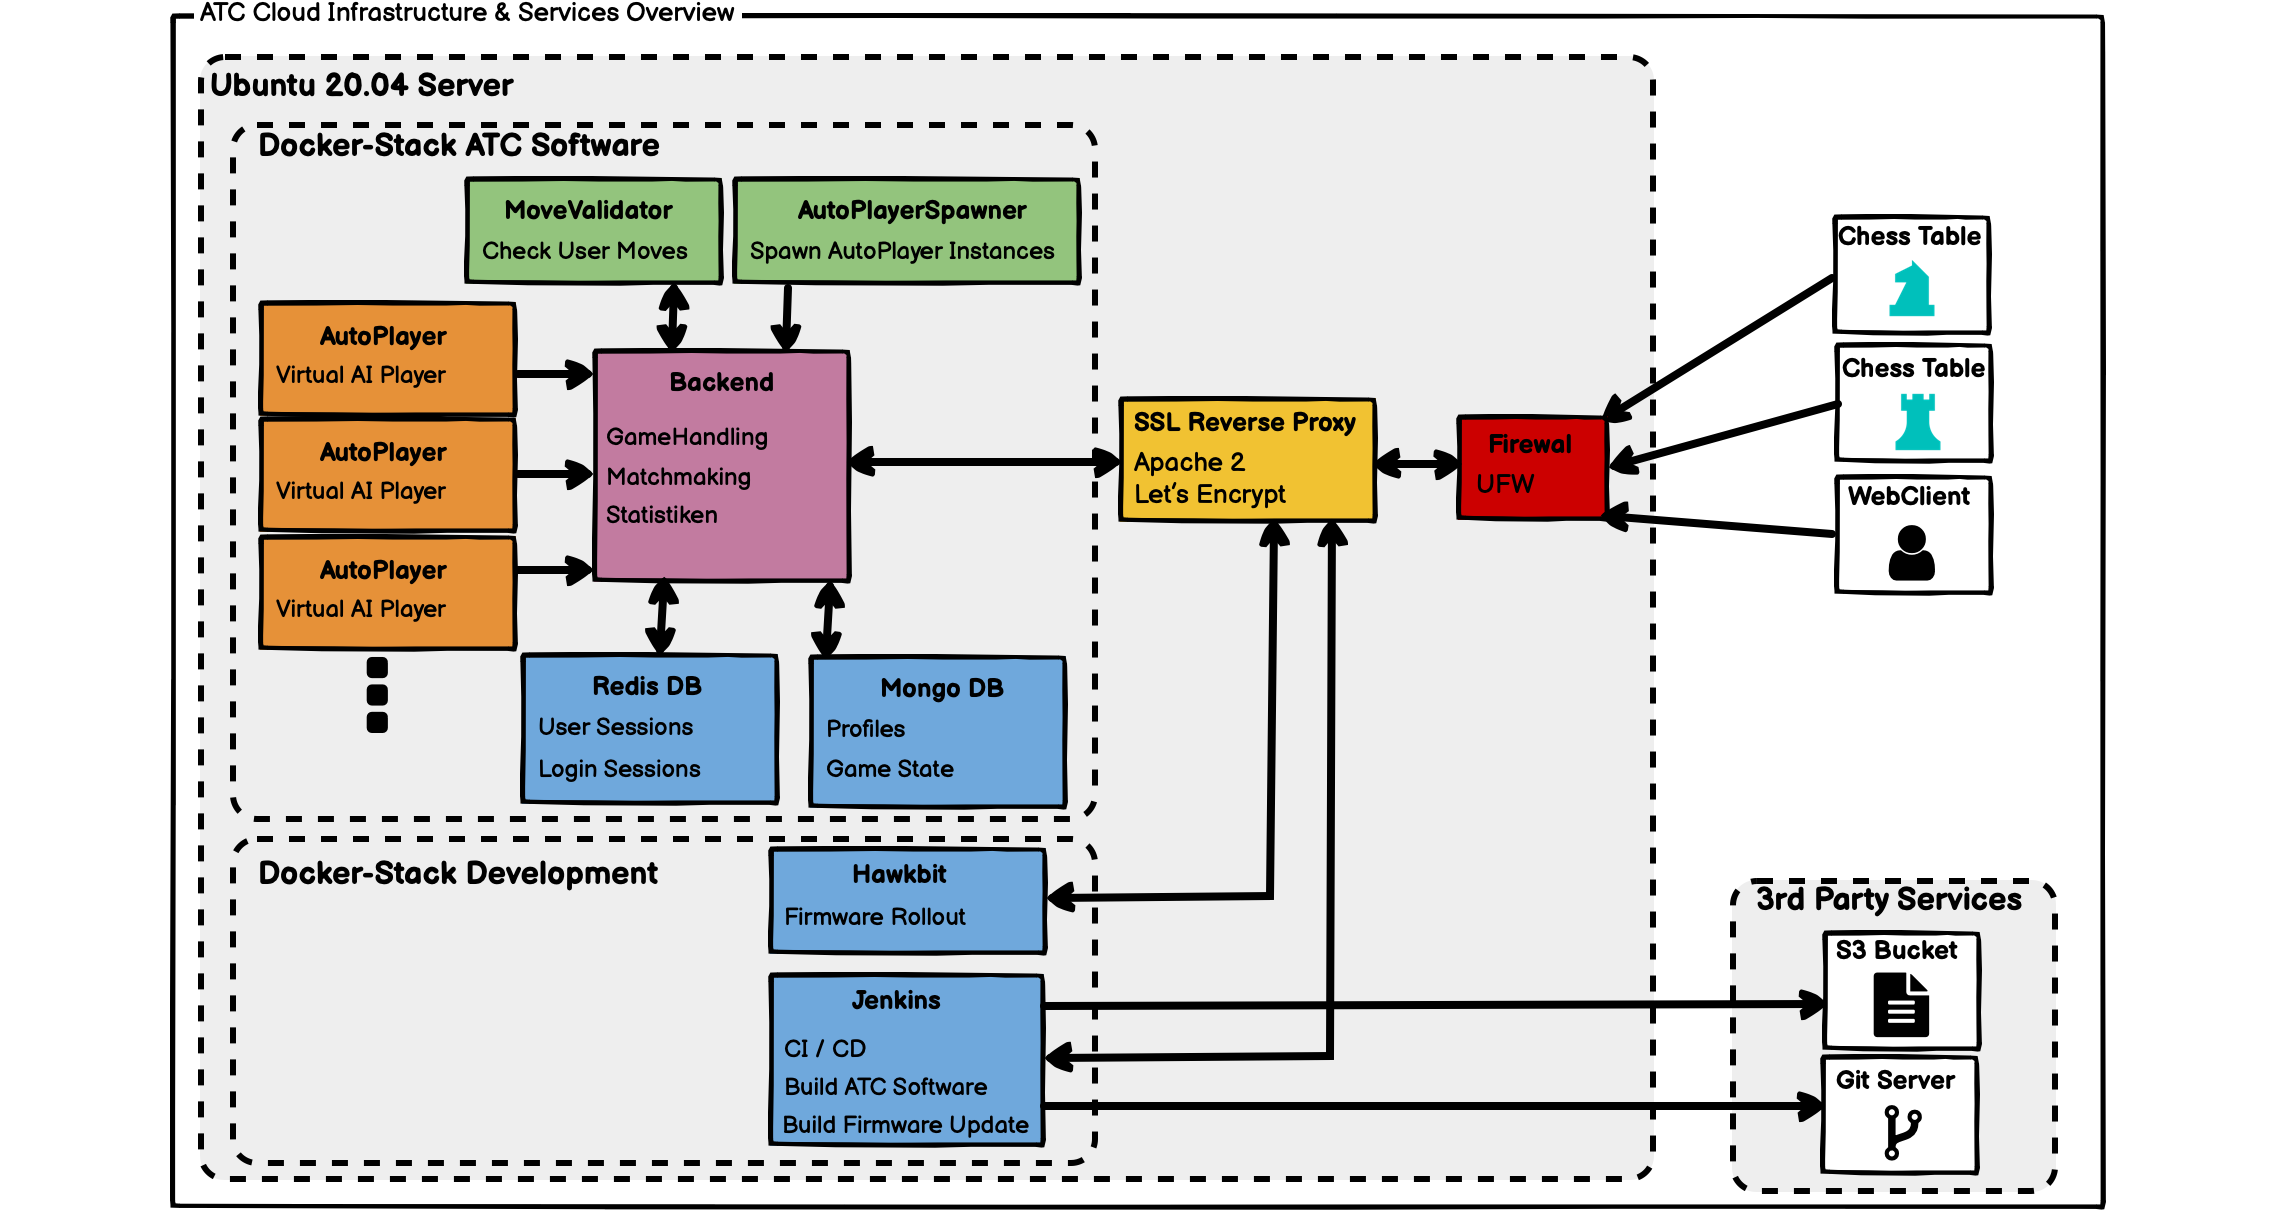
\includegraphics{images/ATC_Cloud_Architecture.png}
\caption{Gesamtübersicht der verwendeten Cloud-Infrastruktur
\label{ATC_Cloud_Architecture}}
\end{figure}

\hypertarget{api-design}{%
\section{API Design}\label{api-design}}

Das System soll so ausgelegt werden, dass es zu einem späteren Zeitpunkt
mit verschiedenen Client-Devices mit diesem kommunizieren können. Dazu
zählen zum einen der autonome Schachtisch, aber z.B. auch einen
Web-Client, welcher die Funktionalität eines Schachtisches im Browser
abbilden kann. Hierzu muss das System eine einheitliche
\gls{rest}-Schnittstelle bereitstellen.

\begin{figure}
\centering
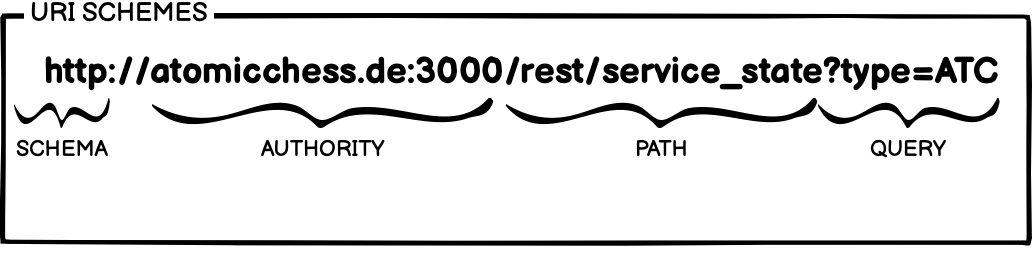
\includegraphics{images/ATC_URI_SCHEMES.png}
\caption{Cloud-Infrastruktur: Aufbau einer URI \label{ATC_URI_SCHEMES}}
\end{figure}

Die RESTful API stellt verschiedene Ressourcen bereit, welche durch eine
URI \ref{ATC_URI_SCHEMES} eindeutig identifizierbar sind. Auf diese
können mittels verschiedenster HTTP Anfragemethoden (GET, POST, PUT,
DELETE) zugegriffen werden. Jeder dieser Methoden stellt einen anderen
Zugriff auf die Ressource dar und beeinflusst somit das Verhalten und
die Rück-Antwort dieser.

Eine URI besteht dabei aus mehreren Teilen. Das Schema gibt an wie die
nachfolgenden Teile interpretiert werden sollen. Dabei wird bei einer
RESTful Schnittstelle typischerweise das \gls{http} Protokoll, sowie
\gls{https} verwendet. Dabei steht \gls{https} für eine verschlüsselte
Verbindung.

Somit stellt die RESTful API eine Interoperabilität zwischen
verschiedenen Anwendungen und Systemen bereit, welche durch ein Netzwerk
miteinander verbunden sind. Dieser Ansatz ist somit geeignet um die
verschiedenen Client Systeme (Schachtisch, Webclient) eine Kommunikation
mit dem Server zu erlauben.

\begin{itemize}
\tightlist
\item
  reverse Proxy für https
\end{itemize}

\hypertarget{service-architektur}{%
\section{Service Architektur}\label{service-architektur}}

\begin{itemize}
\tightlist
\item
  was ist ein Service
\item
  microservice ansatz
\item
  Kapselung der Schach spiel spzifischen funktionaliutäten
\item
  verwendung von NoSQL Datenbanken somit müssen Tabellen nicht spziell
  auf Schach spezifische Felder ausgelegt sein
\item
  statelss Diese stellen alle wichtigen Funktionen zum Betrieb des
  autonomen Schachtischs zur verfügung.
\end{itemize}

\begin{figure}
\centering
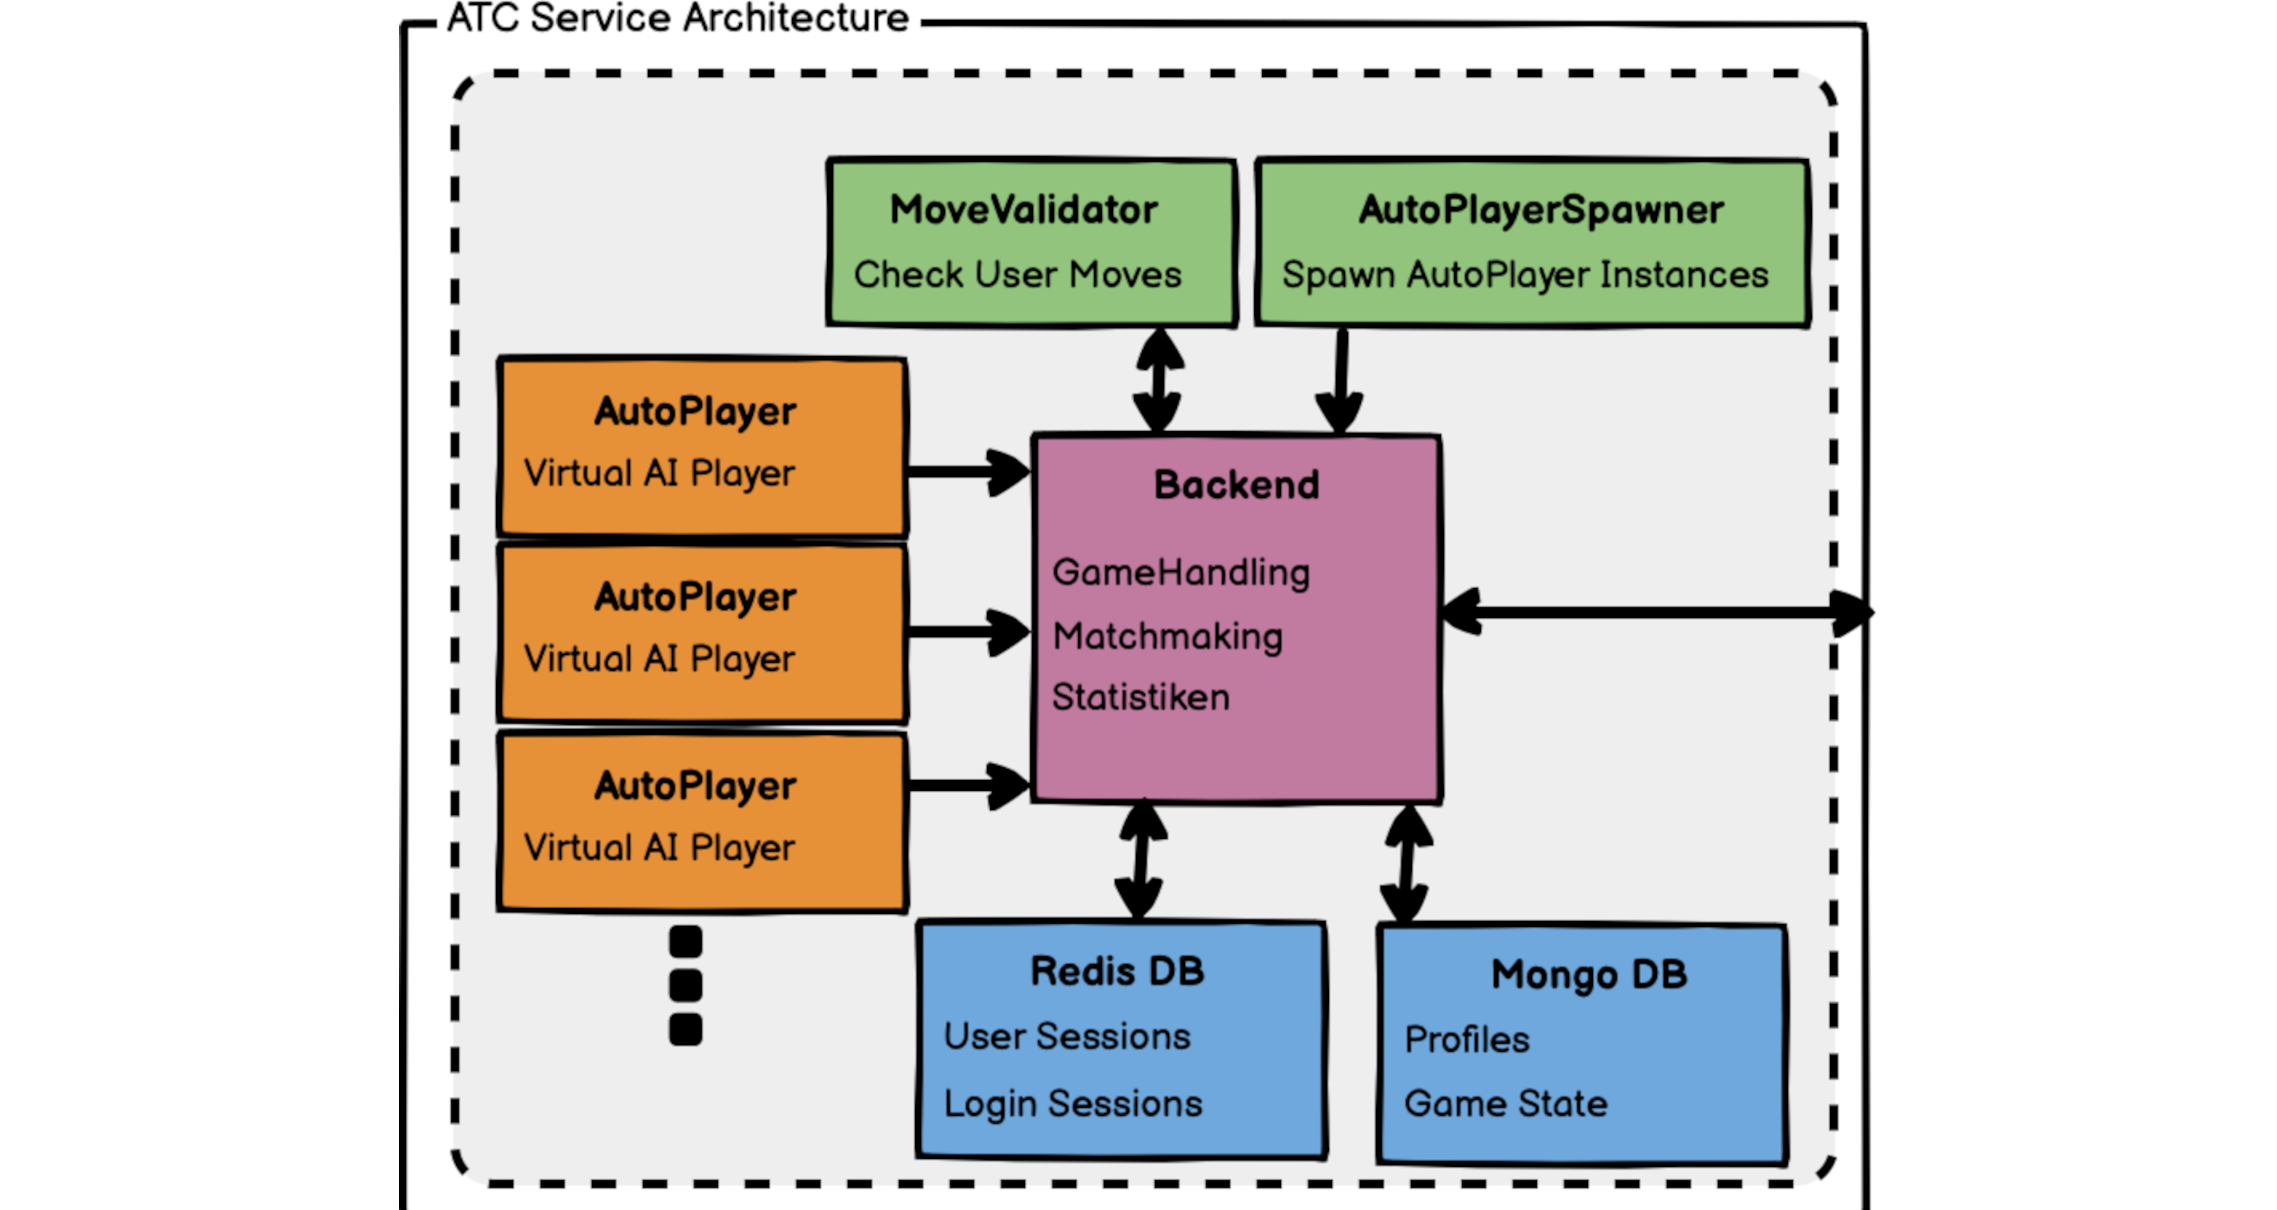
\includegraphics{images/ATC_Service_Architecture.png}
\caption{Cloud-Infrastruktur: Aufbau der Service Architecture
\label{ATC_Service_Architecture}}
\end{figure}

\hypertarget{voruxfcberlegungen}{%
\section{Vorüberlegungen}\label{voruxfcberlegungen}}

\begin{itemize}
\tightlist
\item
  welche funktionalitäten müssen abgedeckt werden
\item
  client aktivitendiagram
\end{itemize}

\hypertarget{backend}{%
\section{Backend}\label{backend}}

\begin{figure}
\centering
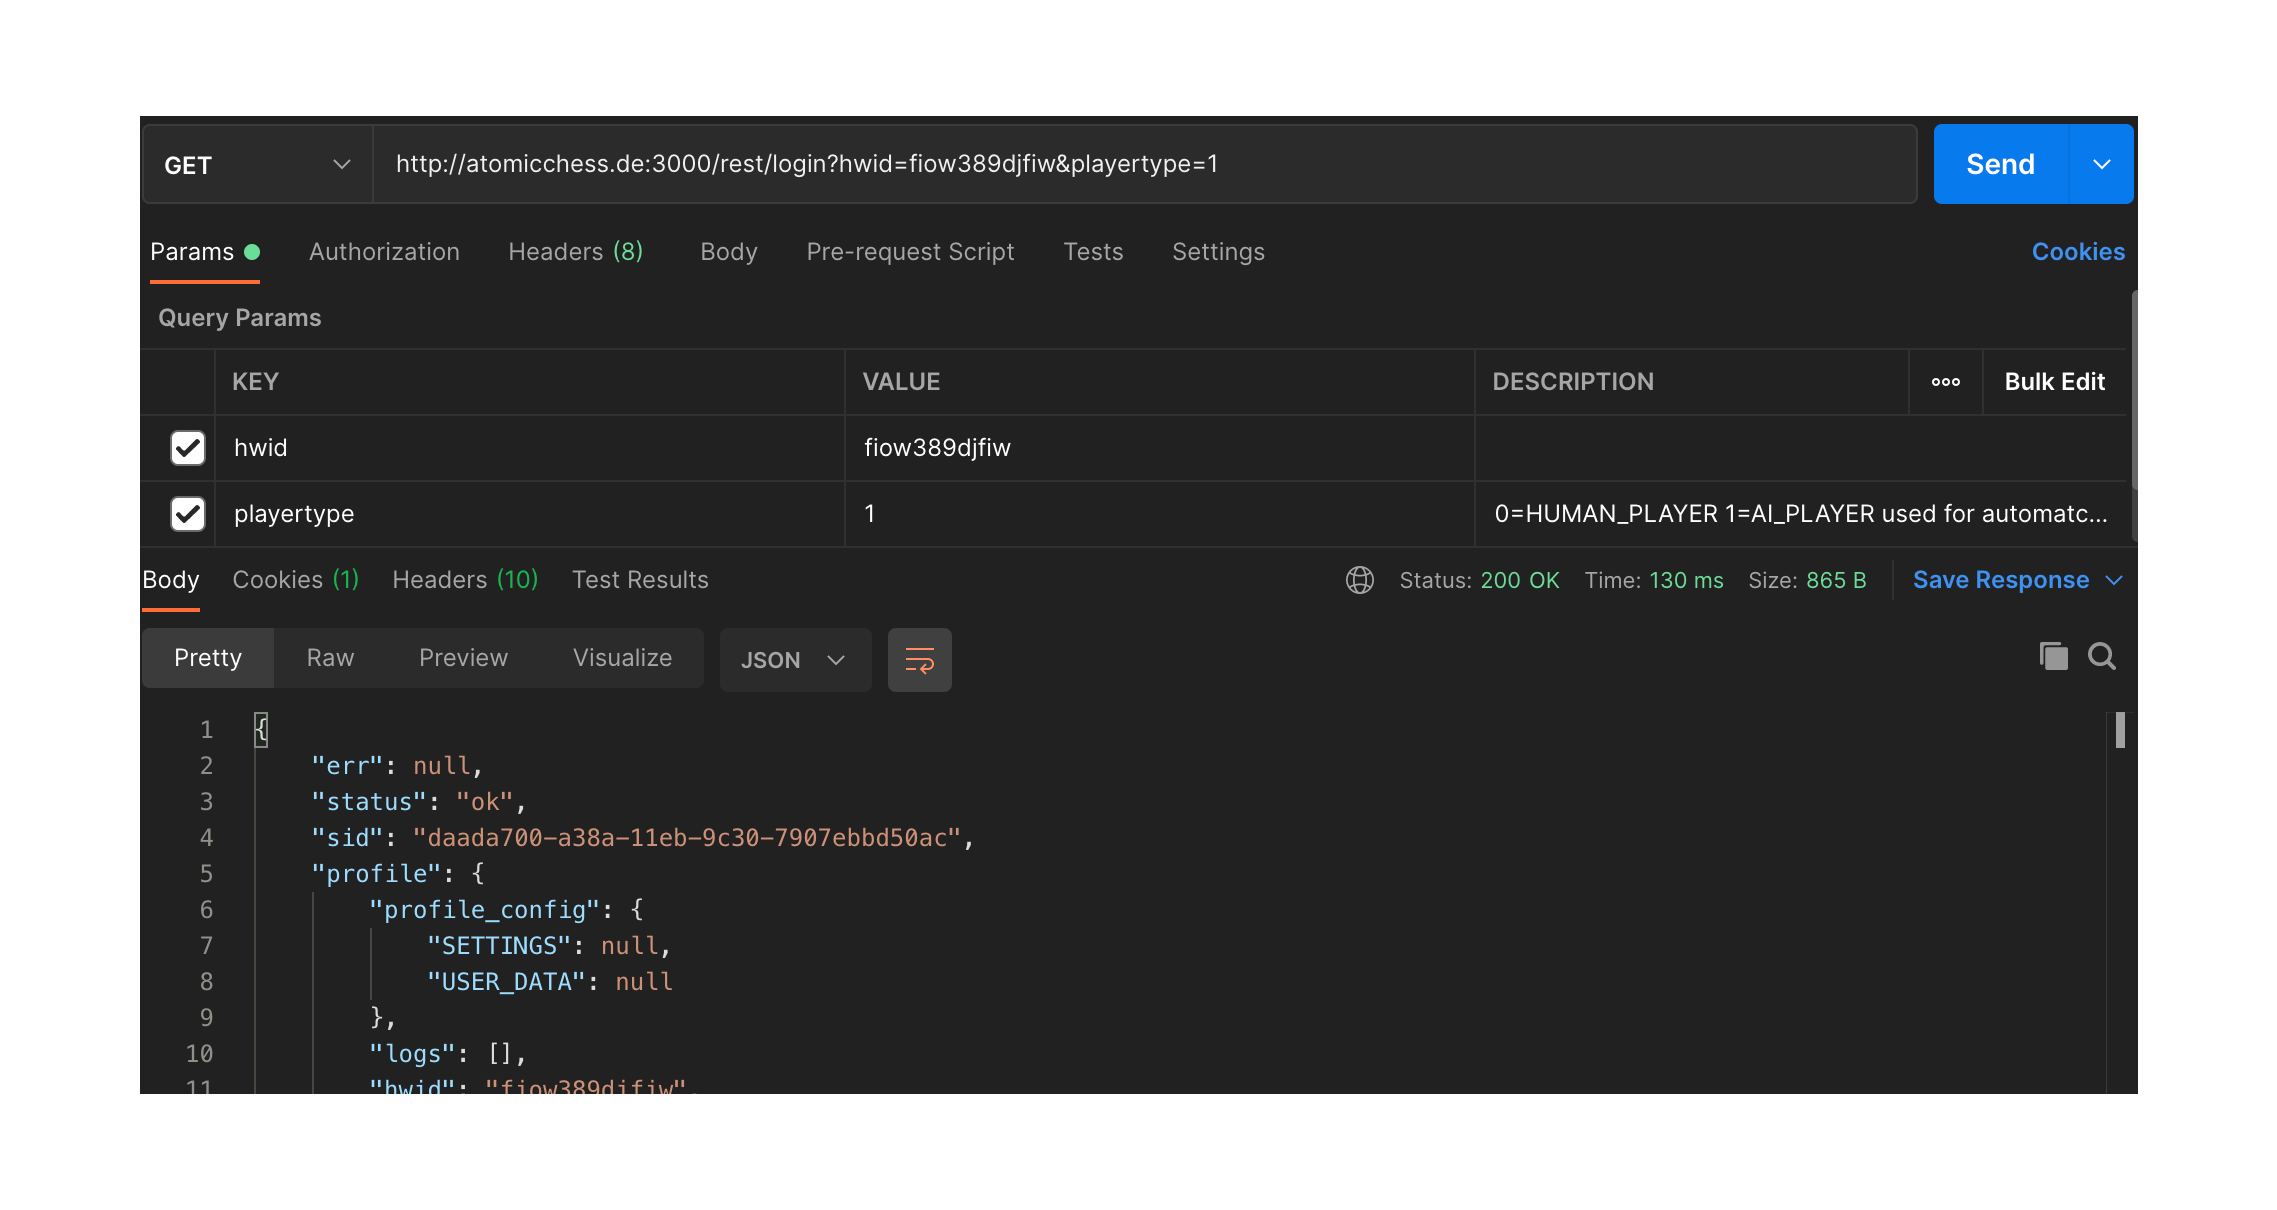
\includegraphics{images/ATC_request_example.png}
\caption{Cloud-Infrastruktur: Backend Login-Requst und Response
\label{ATC_request_example}}
\end{figure}

\begin{itemize}
\tightlist
\item
  matchmaking schachlogik
\item
  zentraler zugriffspunkt auf das System und stellt diese abi bereit
\item
  stellt spielerprofile aus datenbanken bereit bereit
\item
  authentifizierung der clients und deren sessions
\item
  weiterleitung der von spielerinteraktionen an move validator
\item
  spielfelder werden als string übermittelt = hier fen representation;
  einfach zu parsen; standart
\end{itemize}

\hypertarget{movevalidator}{%
\section{MoveValidator}\label{movevalidator}}

Der MoveValidator-Service bildet im System die eigentliche Schachlogik
ab. Die Aufgabe ist es, die vom Benutzer eingegebenen Züge auf
Richtigkeit zu überprüfen und auf daraufhin neuen Spiel-Status
zurückzugeben. Dazu zählen unter anderem das neue Schachbrett und ob ein
Spieler gewonnen oder verloren hat.

Bevor ein Spiel begonnen wird, generiert der MoveValidator das initiale
Spielfeld und bestimmt den Spieler, welcher als erstes am Zug ist.

\begin{figure}
\centering
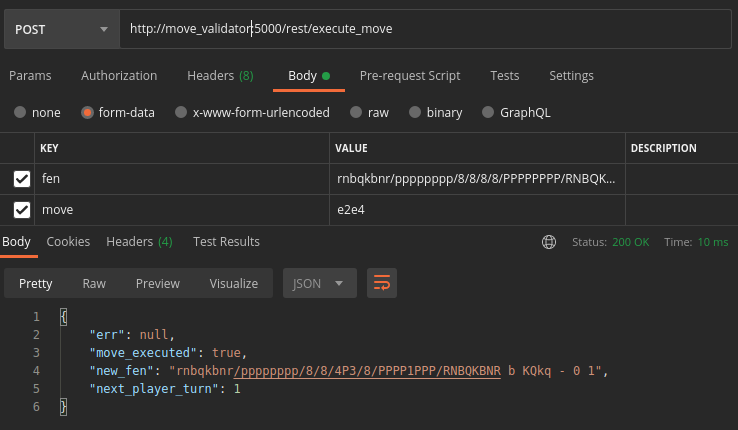
\includegraphics{images/ATC_movevalidator_execute_move.png}
\caption{MoveValidator: Beispiel Request zur Ausführung eines Zuges auf
einem gegebenen Schachbrett \label{ATC_movevalidator_execute_move}}
\end{figure}

Der Backend-Service fragt ein neues Spiel an oder übergibt einen
Schachzug inkl. des aktuellen Spielbrett-Aufbaus an den
Service.\ref{ATC_movevalidator_execute_move} Der Response wird dann vom
Backend in der Datenbank gespeichert und weiter an die Client-Devices
verteilt.

\begin{longtable}[]{@{}llll@{}}
\caption{MoveValidator-Service \gls{api} Overview}\tabularnewline
\toprule
MoveValidator \gls{api} & \gls{api}-Route & Method &
Form-Data\tabularnewline
\midrule
\endfirsthead
\toprule
MoveValidator \gls{api} & \gls{api}-Route & Method &
Form-Data\tabularnewline
\midrule
\endhead
Check Move & /rest/check\_move & POST & * fen * move *
player\tabularnewline
Execute Move & /rest/execute\_move & POST & fen * move\tabularnewline
Validate Board & /rest/validate\_board & POST & fen\tabularnewline
Init Board & /rest/init\_board & GET &\tabularnewline
\bottomrule
\end{longtable}

Allgemein geschieht die Kommunikation über vier \gls{api} Calls, welche
vom MoveValidator-Service angeboten werden. Als erstes wird vom Backend
der \passthrough{\lstinline!/rest/init\_board!} Request verwendet,
welcher ein neues Spielbrett in der \gls{fen} Notation zurückgibt,
welches zum Start der Partie verwendet wird. Allgemein arbeitet wurde
das komplette System so umgesetzt, dass dieses mit einem Spielfeld in
einer Zeichenketten/String arbeitet. Dies hat den Vorteil, dass die
Spielfeld-Notation leicht angepasst werden kann. Mit diesem Design ist
es möglich, auch andere Spielarten im System zu implementieren, da nur
an dieser Stelle die initialen Spielfelder generiert werden und Züge der
Spieler validiert werden müssen.

Die \gls{fen} Notation ist universal und kann jede Brettstellung
darstellen. Auch enthält diese nicht nur die Figur Stellungen, sondern
auch weitere Informationen, wie die aktuelle Nummer des Zuges oder
welcher Spieler gerade an der Reihe ist. Diese werden dann in der
\gls{xfen} Notation angegeben, bei der zusätzlich zu der Brettstellung
auch noch die weiteren Informationen angehängt werden.

\begin{longtable}[]{@{}ll@{}}
\caption{Vergleich \gls{fen} - \gls{xfen}}\tabularnewline
\toprule
FEN-TYPE & FEN-String\tabularnewline
\midrule
\endfirsthead
\toprule
FEN-TYPE & FEN-String\tabularnewline
\midrule
\endhead
FEN & rnbqkbnr/pp1ppppp/8/2p5/4P3/5N2/PPPP1PPP/RNBQKB1R\tabularnewline
X-FEN & rnbqkbnr/pp1ppppp/8/2p5/4P3/5N2/PPPP1PPP/RNBQKB1R b KQkq - 1
2\tabularnewline
SCHEMA & Board Player-Color Rochade En-Passant Halfturn
Turn-Number\tabularnewline
\bottomrule
\end{longtable}

Alle gängigen Schachprogramme und Bibliotheken unterstützen das Laden
von Spielbrettern in der \gls{fen} bzw \gls{xfen} Schreibweise, ebenso
die für den MoveValidator Service verwendete Python-Chess Bibliothek
\cite{pythonchesslib}. Diese unterstützt zusätzlich die Generierung
der für den Benutzer möglichen Schachzügen, welche auf dem aktuellen
Brett möglich sind.

Diese Liste wird vom System dazu verwendet, um sicherzustellen, dass der
Benutzer nur gültige Züge tätigen kann. Diese Funktion lässt sich
zusätzliche abschalten, falls das Spiel nicht nach den allgemeinen
Schachregeln verlaufen soll. Bei der Generierung der möglichen
Schachzüge muss zwischen den Legal-Moves und den Pseudo-Legal
Schachzügen unterschieden werden. Die Legal-Moves beinhalten nur die
nach den Schachregeln möglichen Zügen, welche von Figuren des Spielers
ausgeführt werden können. Die Pseudo-Legal Schachzüge sind alle
Schachzüge, welche von den Figuren auf dem aktuellen Schachbrett möglich
sind; darin sind unter anderem auch alle anderen Figur-Züge enthalten,
solange der König des aktuellen Spielers sich aktuell auf dem
Schachbrett befindet.

Wenn ein Spieler an der Reihe ist und einen Zug getätigt hat, wird sein
getätigter Zug mittels der \passthrough{\lstinline!/rest/check\_move!}
\gls{api} überprüft und festgestellt, ob dieser gemäß der Legal-Moves
durchführbar war. Ist dies der Fall, wird der Zug auf dem
onlie-Spielbrett angewendet. Dies geschieht durch die
\passthrough{\lstinline!/rest/execute\_move!} \gls{api}. Diese führt den
Zug aus, ermittelt anschließend das neue Spielbrett und überprüft
zusätzlich, ob das Spiel gewonnen oder verloren wurde.

Hat der Benutzer jedoch einen ungültigen Zug ausgeführt, wird dieser vom
System storniert und der Client des Benutzers stellt den Zustand des
Spielbretts vor dem getätigten Zug wieder her. Danach hat der Benutzer
die Möglichkeit einen alternativen Zug auszuführen.

\hypertarget{entwicklung-webclient}{%
\section{Entwicklung Webclient}\label{entwicklung-webclient}}

\begin{figure}
\centering
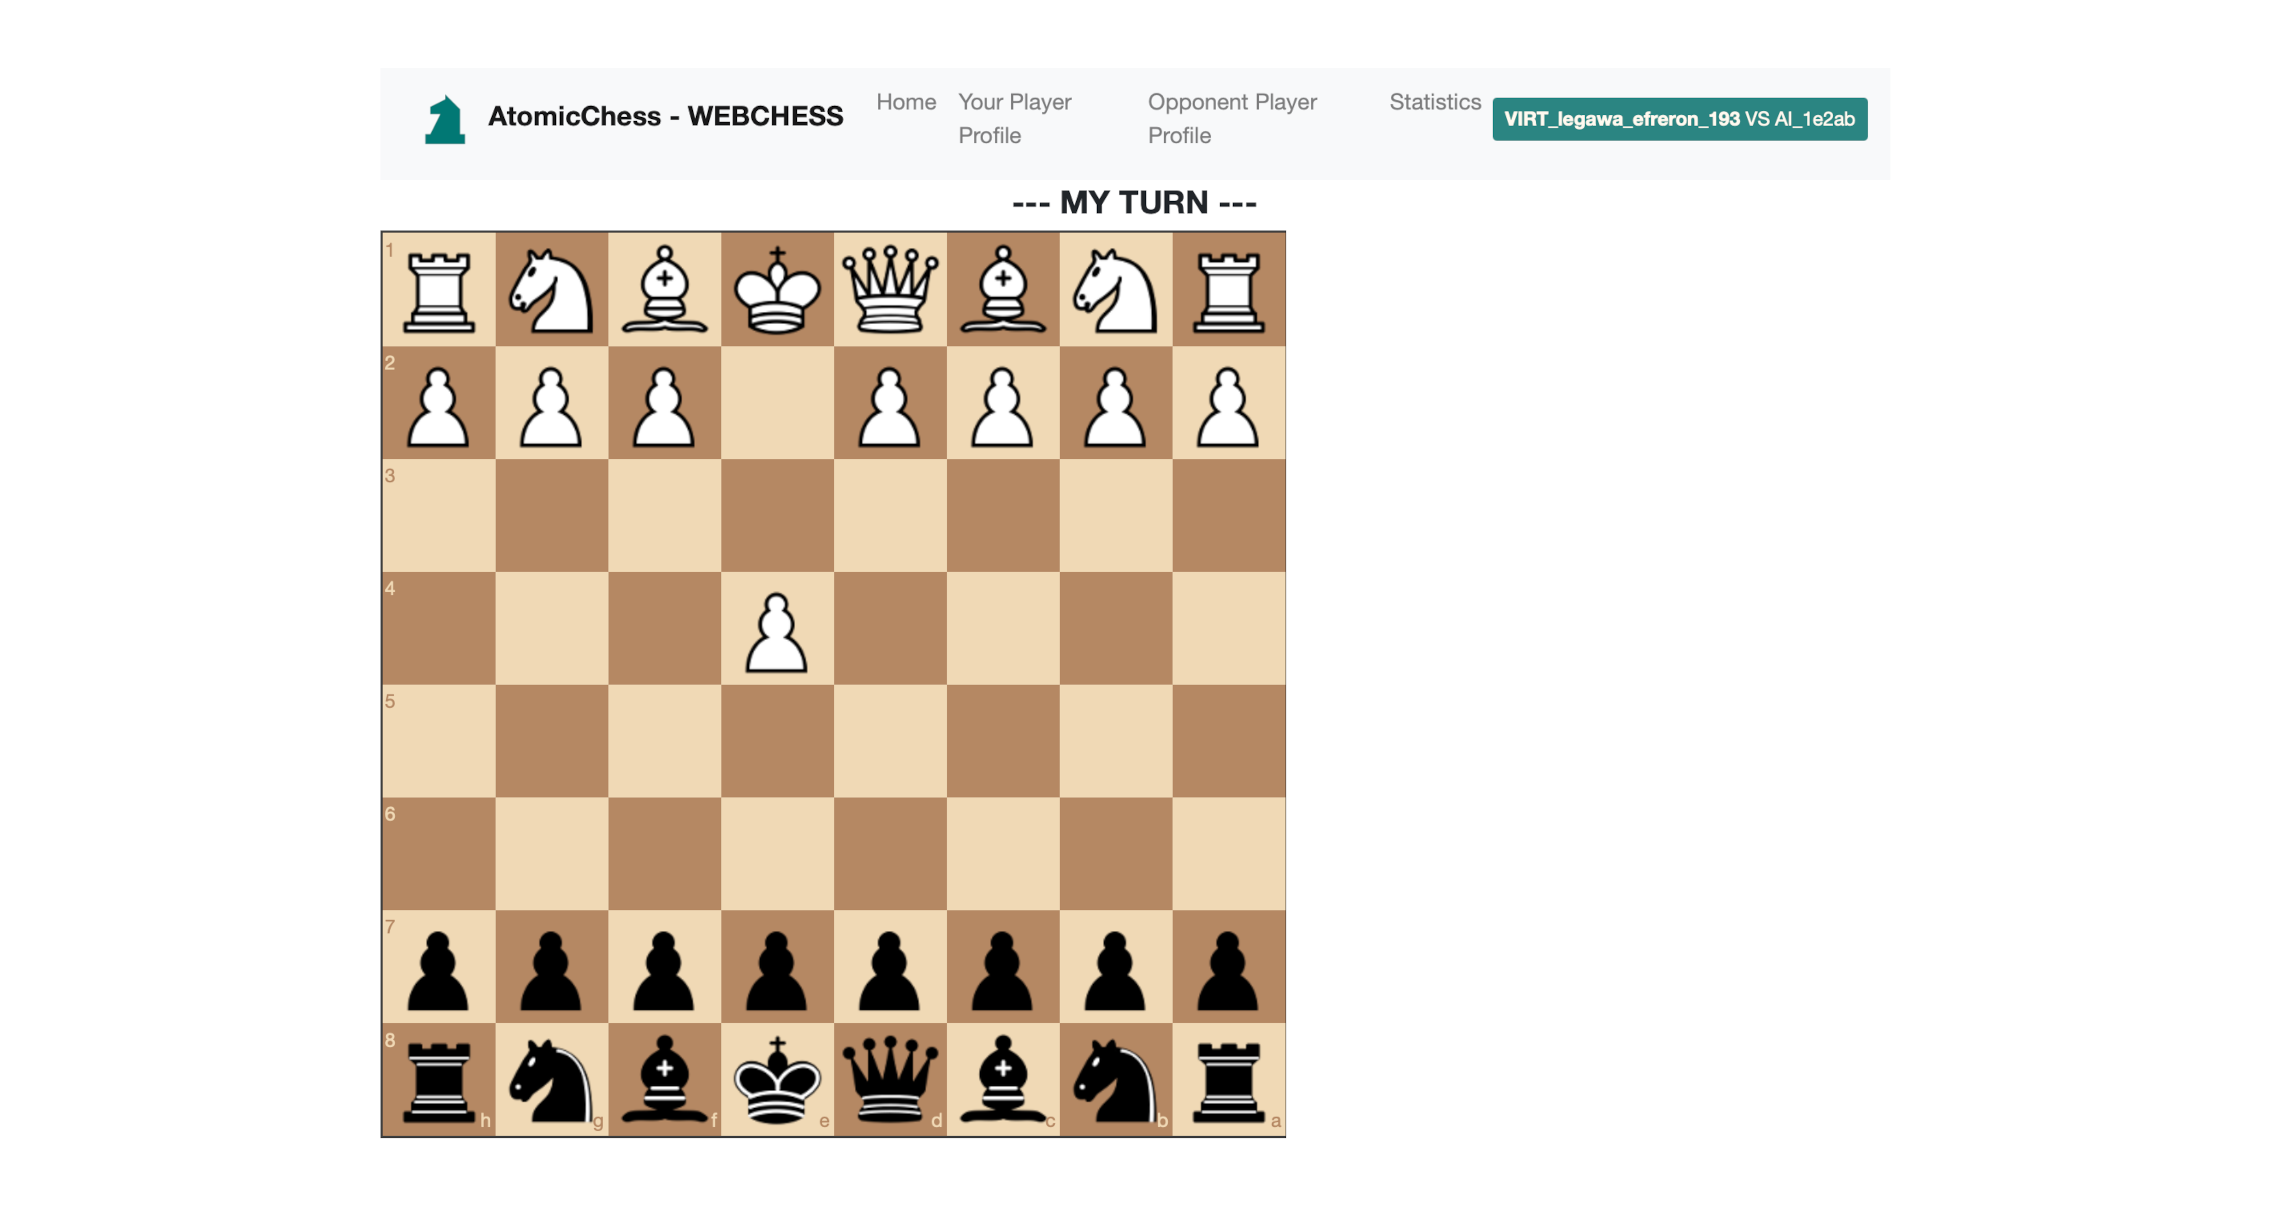
\includegraphics{images/ATC_webclient.png}
\caption{Webclient: Spielansicht \label{ATC_webclient}}
\end{figure}

Der Webclient wurde primär dazu entwickelt, um das System während der
Entwicklung zu testen. Dieser simuliert einen autonomen Schachtisch und
verwendet dabei die gleichen \gls{http} Requests. Um das zu ermöglichen
wurde dieser vollständig in \gls{js} umgesetzt im Zusammenspiel mit
\gls{html} und \gls{css} und ist somit komplett im Browser ausführbar.

Ausgeliefert werden die statischen Dateien zur Einfachheit durch den
Backend-Service; es wurde kein gesonderter Frontend-Service angelegt.
Durch die Implementierung des Webclienten in \gls{js} ist dieser sogar
lokal über einen Browser ausführbar, ohne dass die benötigten Dateien
über einen Webserver ausgeliefert werden müssen.

Zusätzlich zu dem verwendeten Vanilla-\gls{js} wurde jQuery als
zusätzliche \gls{js} Bibliothek verwendet, welches eine Manipulation der
\gls{html} Elemente stark vereinfacht. Diese bietet insbesondere einfach
zu nutzende HTTP-Request Funktionen bzw. \gls{ajax} an, welche für die
Kommunikation mit dem Backen-Service verwendet werden. Diese werden im
Hintergrund eingesetzt, sodass der Webclient automatisch den neuen
Spielzustand dem Benutzer anzeigt. Dies geschieht mittels
\passthrough{\lstinline!polling!}, bei dem der Webbrowser in zyklischen
Abständen die aktuellen Spiel-Informationen vom Backen-Service abfragt.
Diese Methode wurde verwendet, um eine maximale Kompatibilität mit
verschiedensten gegebenenfalls älteren Web-Browsern sicherzustellen.
Eine moderne alternative ist die Verwendung von Web-Sockets, bei welcher
der Web-Browser eine direkte TCP-Verbindung zum Webserver (in diesem
Fall der Backend-Service) aufnehmen und so eine direkte Kommunikation
stattfinden kann ohne Verwendung der
\passthrough{\lstinline!polling!}-Methode.

Der Hauptanwendungsfall des Webclienten während der Entwicklung ist es,
weitere Spieler zu simulieren und so ein Spiel mit nur einem autonomen
Schachtisch testen zu können. Durch den Webclient ist zusätzliche
möglich, gezielt Spiele und Spielzüge zu simulieren. Hierzu gehören vor
allem Sonderzüge wie die Rochade oder der En-Passant Zug. Auch können
durch den Webclient ungültige Züge simuliert werden, welche durch die
Verwendete Schach-AI nicht getätigt werden.

Während der Implementierung wurde der Webclient weiter ausgebaut und es
wurde weitere Eigenschaften ergänzt. Dazu zählt zum einen eine Übersicht
über vergangene und aktuell laufende Spiele. In dieser können Spiele Zug
um Zug nachvollzogen werden und weitere Information über den Spielstatus
angezeigt werden.\ref{ATC_statistics} Auch ist es möglich, aktuell
laufende Spiele in Echtzeit anzeigen zu lassen; somit wurde eine
Livestream-Funktionalität implementiert.

\begin{figure}
\centering
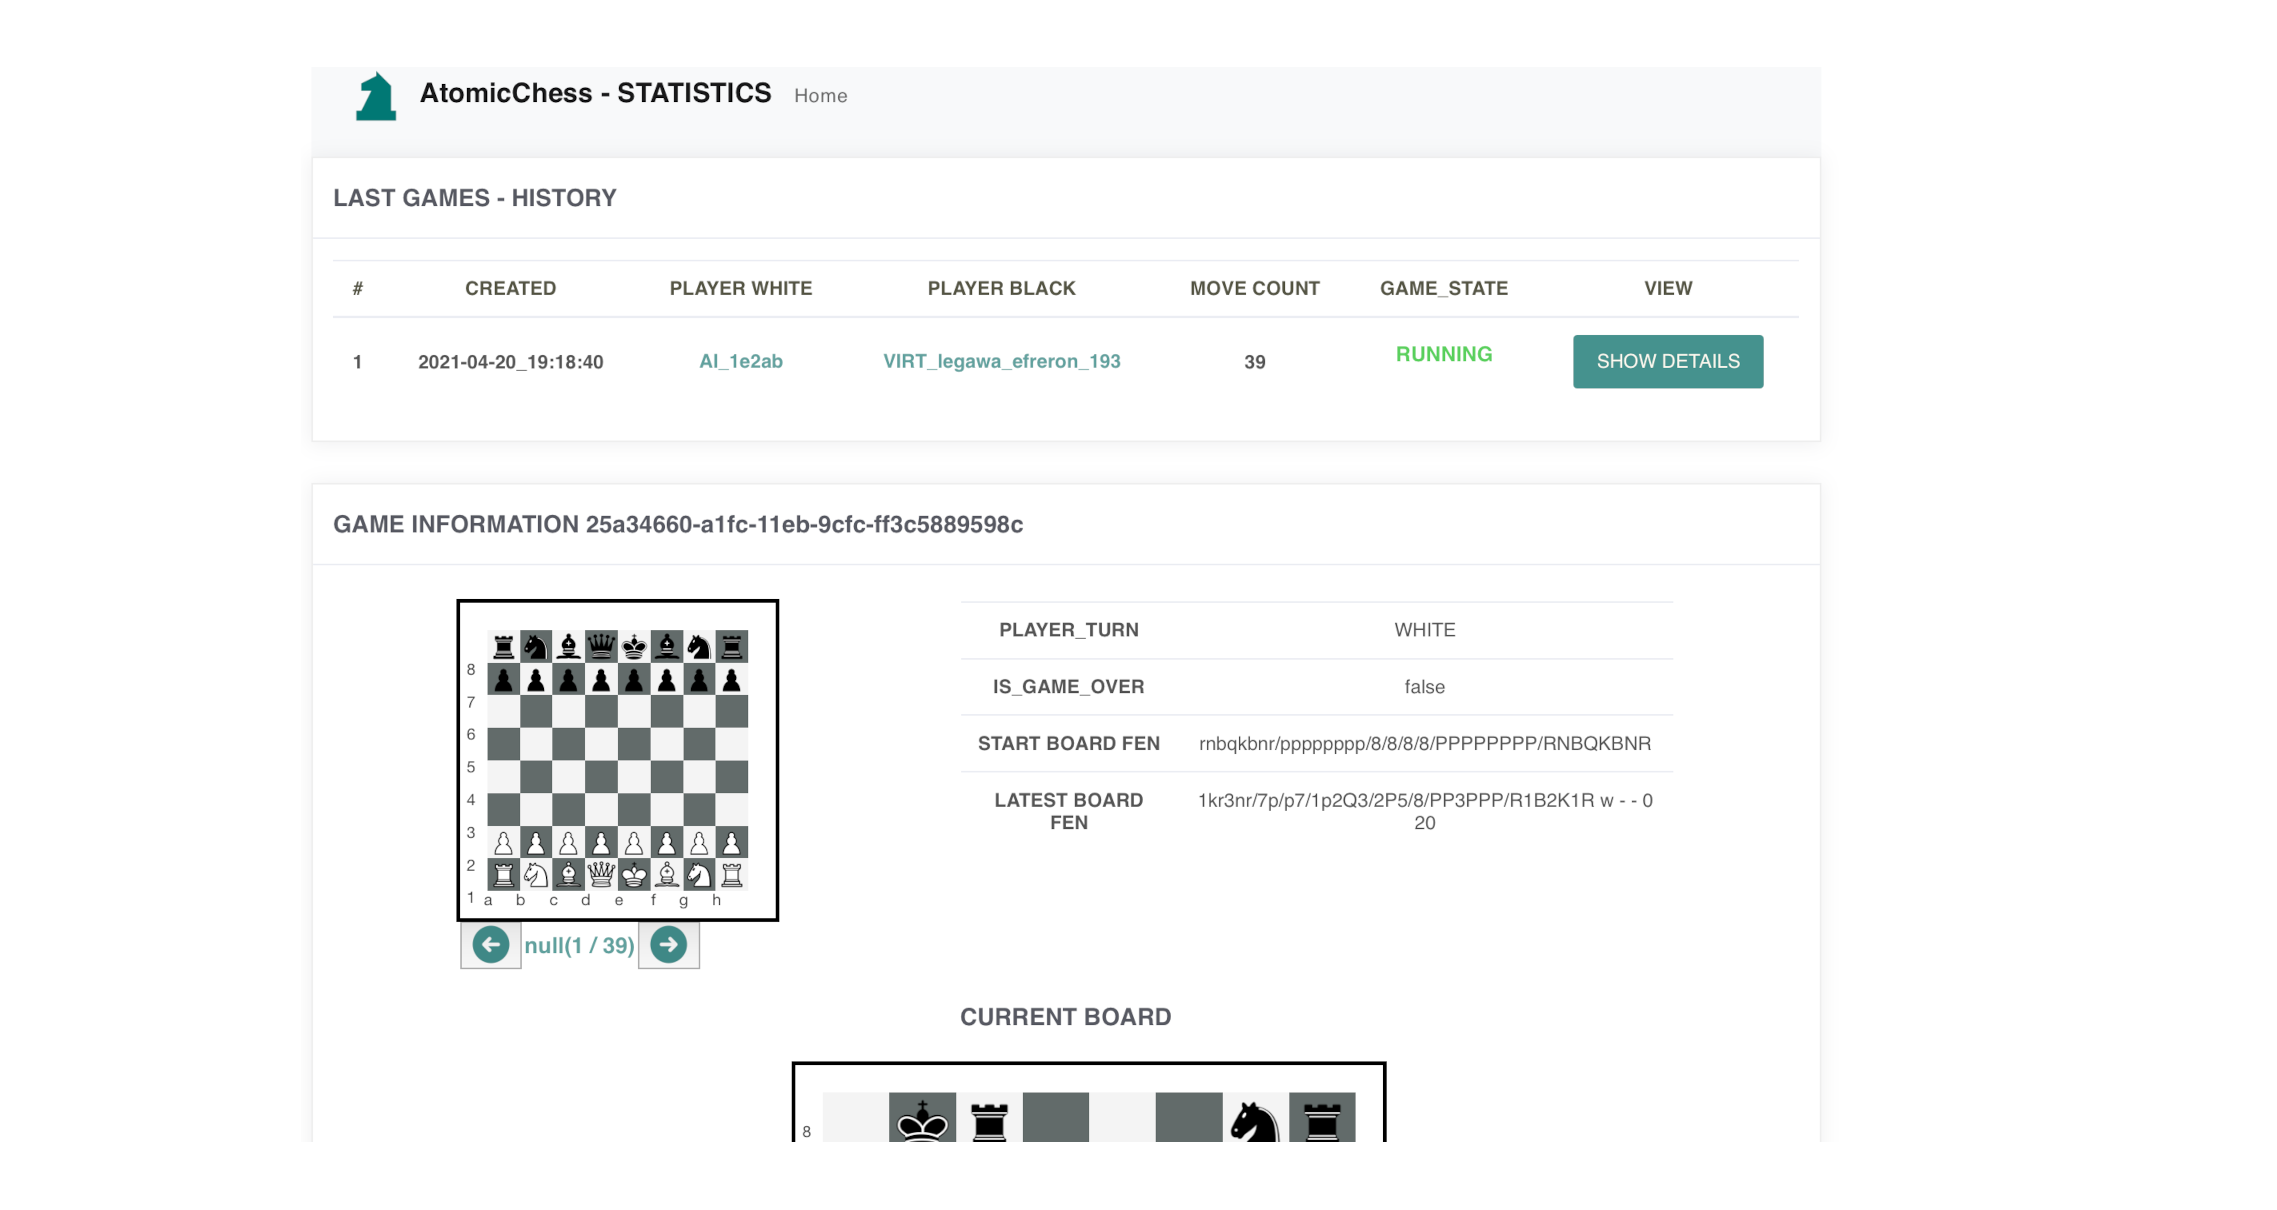
\includegraphics{images/ATC_statistics.png}
\caption{Webclient: Statistiken \label{}}
\end{figure}

\hypertarget{autoplayer}{%
\section{AutoPlayer}\label{autoplayer}}

Der AutoPlayer-Service stellt den Computerspieler bereit.

Jede Service-Instanz stellt einen virtuellen Spieler bereit, welcher die
gleichen Schnittstellen wie der Webclient oder der autonome Schachtisch
verwendet. Die einzige Änderung an den verwendeten \gls{rest}-Calls ist
der Login-Requst. Hier wird das \passthrough{\lstinline!playertype!}
Flag gesetzt welches den Spieler als Computerspieler gegenüber dem
System authentifiziert. Daraus resultierend wird dieser während des
Matchmaking-Prozesses erst für ein Match ausgewählt, wenn keine anderen
menschlichen Spieler mehr zur Verfügung stehen. Dieser digitale
Gegenspieler ist vom Typ Webclient oder autonomer Schachtisch. Dieser
Prozess gewährleistet zudem, dass immer zuerst die menschlichen Spieler
ein Spiel beginnen und die digitalen nur Alternativen darstellen.

Eine weitere Modifikation ist die Verwendung einer Schach-AI, da dieser
Service als Computerspieler agieren soll. Hierzu kam die Open-Source
Chess Engine Stockfish\cite{stockfish} in der Version 11 zum
Einsatz. Die Stockfish-Engine bietet noch weitere Features, als nur die
nächstbesten Züge zu einem gegebenen Schachbrett zu ermitteln.

Die AutoPlayer-Instanz kommuniziert über das \gls{uci}
Protokoll\cite{uciprotocol} mit der Engine. Dieses Protokoll wird in
der Regel von Schach-Engines verwendet, um mit einer \gls{gui} zu
kommunizieren.

Um das aktuelle Spielbrett in der Engine zu setzten wird dieses in der
\gls{xfen} Notation mit dem Prefix
\passthrough{\lstinline!position fen!} als Klartext an die Engine
übergeben und sendet daraufhin eine List möglicher Züge zurück. Der
erste Index dieser Liste ist dabei der am besten bewerteten Zug der
Engine.

Im Kontext des AutoPlayer-Service wird der Engine nur das aktuelle
Spielbrett übermittelt und der nächstbeste Zug auslesen. Dies wird
ausgeführt, wenn der AutoPlayer am Zug ist. Nachdem die Engine einen
passenden Zug gefunden hat, wird das Ergebnis über den
\passthrough{\lstinline!make\_move!} \gls{rest}-API Call übermittelt.

Wenn das Match beendet wird, beendet sich auch die Service-Instanz.
Diese wird jedoch wieder gestartet, wenn die Anzahl der zur Verfügung
stehenden Computerspieler unter einen definierten Wert fallen. Somit ist
dafür gesorgt, dass das System nicht mit ungenutzten
AutoPlayer-Instanzen gebremst wird. Diese Anzahl \ref{ai_player_count}
ist in der Konfiguration des Backend-Service frei wählbar und kann je
nach zu erwarteten Aufkommen angepasst werden.

Allgemein skaliert das System durch diese Art der Ressourcenverwaltung
auch auf kleinen Systemen sehr flexibel. Durch die Art der
Implementierung, dass sich der AutoPlayer-Service wie ein normaler
Spieler verhält, sind auch andere Arten des Computerspieler möglich. So
ist es zum Beispiel möglich, die Spielstärke je Spieler anzupassen oder
einen Computerspieler zu erstellen, welcher nur zufällige Züge zieht.

Ein weiterer Anwendungsfall für den AutoPlayer-Service, ist das Testen
des weiteren Systems insbesondere des Backend-Service. Durch das
Erstellen eines Spiels mit zwei AutoPlayer-Instanzen, können
automatisierte Schachpartien ausgeführt werden um die Funktionsfähigkeit
des restlichen Systems zu testen. Diese Feature wurde insbesondere bei
der Entwicklung des Webclient und der Steuerungssoftware für den
autonomen Schachtisch verwendet.

\hypertarget{embedded-system-software}{%
\chapter{Embedded System Software}\label{embedded-system-software}}

\begin{itemize}
\tightlist
\item
  Hauptsoftware zur Steuerung der Elektrik/Mechanik
\item
  Kommunikation mit dem Cloud-Server
\end{itemize}

\hypertarget{ablaufdiagramm}{%
\section{Ablaufdiagramm}\label{ablaufdiagramm}}

\begin{itemize}
\tightlist
\item
  dummer/thin Client
\item
  Synchronisierung von gegeben Schachfeld mit dem lokalen Schachfeld
\item
  getätigte züfe werden direkt an den schachserver geschickt und dieser
  generiert daraufhin das neue schachbrett welches von beiden Partner
  sync
\end{itemize}

\begin{figure}
\centering
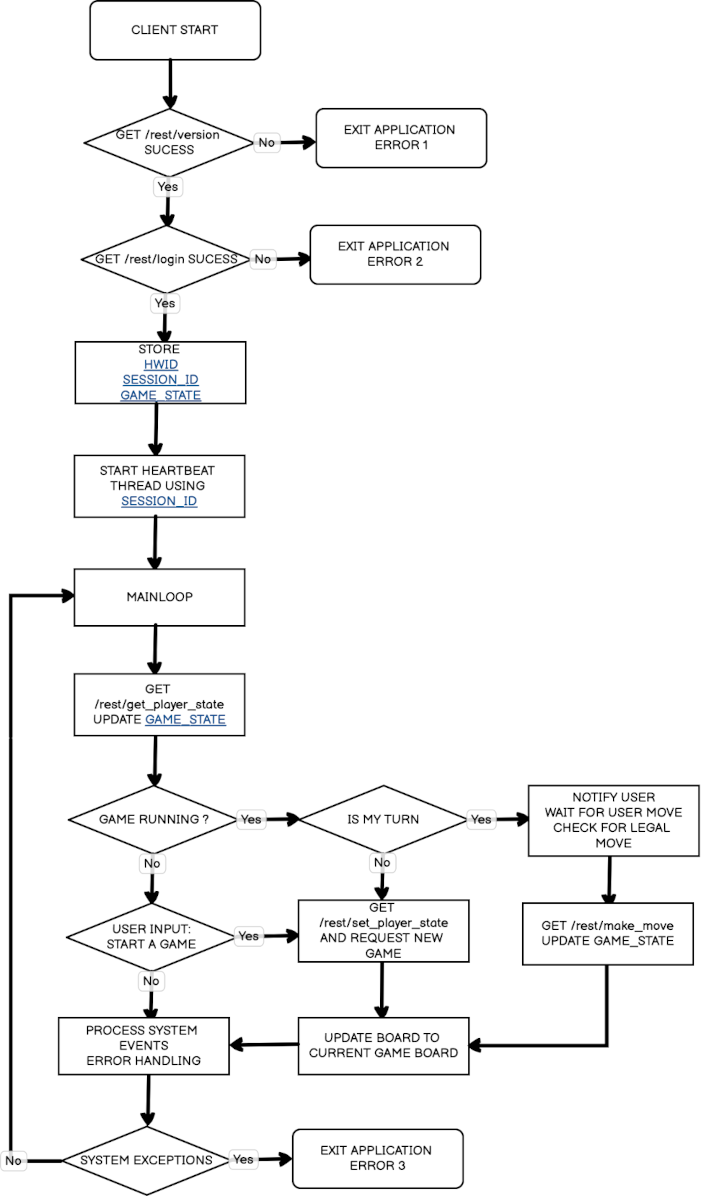
\includegraphics{images/ATC_gameclient_statemachiene.png}
\caption{Embedded System Software: Ablaufdiagramm
\label{ATC_gameclient_statemachiene}}
\end{figure}

\hypertarget{figur-bewegungspfadberechnung}{%
\section{Figur
Bewegungspfadberechnung}\label{figur-bewegungspfadberechnung}}

\begin{itemize}
\tightlist
\item
  Algorithmus zur Umsetzung eines Schachzugs
\item
  Auftrennung in current und target Board
\item
  vier Schritte (entfernen, bewegen, hinzufügen, bewegen) \#\#
  Schachfeld Scan Algorithmus zur Erkennung von Schachzügen
\end{itemize}

\begin{figure}
\centering
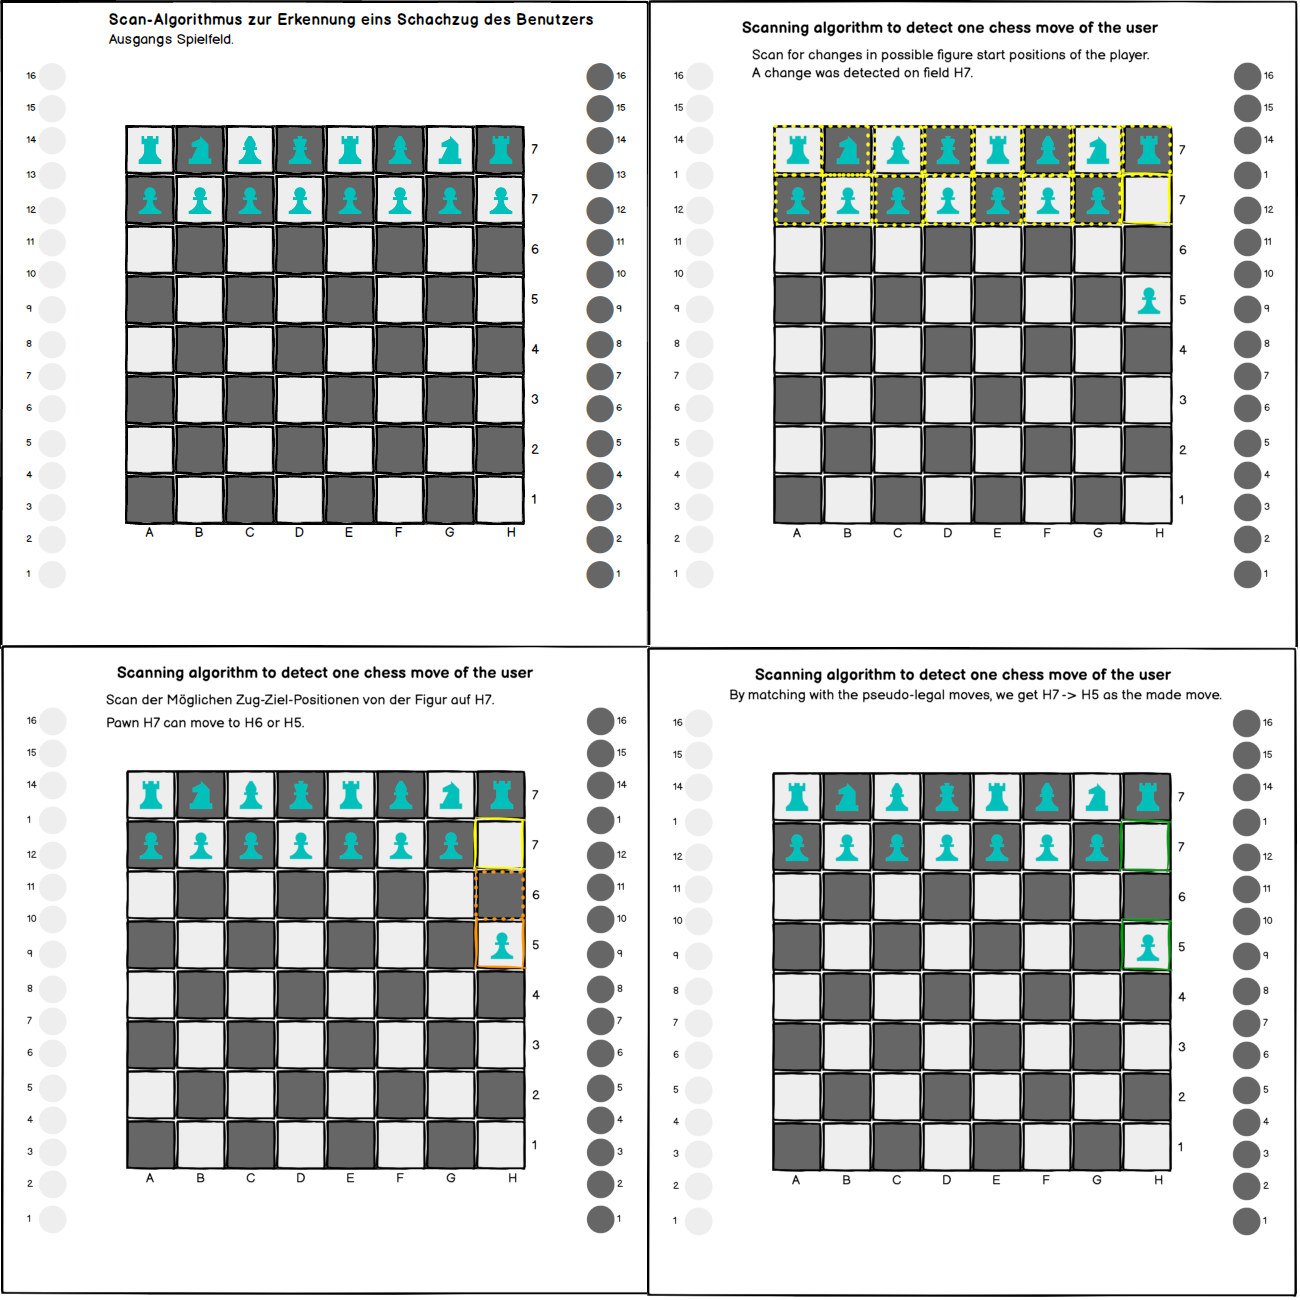
\includegraphics{images/ATC_ChessMoveAlgorithm.png}
\caption{Embedded System Software: Schachfeld Scan Algorithmus Ablauf
\label{ATC_ChessMoveAlgorithm}}
\end{figure}

\begin{itemize}
\tightlist
\item
  Benutzer bestätigt, dass er Schachzug gemacht hat
\item
  Ermittlung des getätigten Schachzugs
\item
  Scan der Schachfeld-Veränderungen, durch Vergleich des vorherigen
  Schachfelds und der möglichen Züge
\end{itemize}

\hypertarget{inter-prozess-communication}{%
\section{Inter Prozess
Communication}\label{inter-prozess-communication}}

Bei der Entwicklung des Systems wurde darauf geachtet, dass sich das
User-Interface austauschen lässt. Somit ist es auch möglich, ein
webbasiertes User-Interface zu integrieren. Dazu wurde ein zusätzliches
\gls{ipc} Layer hinzugefügt, welches eine Abstraktion der von der
User-Interface Software verwendeten Funktionen auf der
Controller-Software Ebene bereitstellt.

Dazu wurde eine einfache \gls{ipc} Bibliothek implementiert, welche dem
Controller- als auch dem User-Interface als Shared-Library zur Verfügung
steht. Diese stellt einfache Funktionen zum Senden und Empfangen von
Events bereit und erzeugt nach der Initialisierung einen separaten
Thread in welcher die Kommunikation mit den anderen \gls{ipc} Instanzen
verwaltet wird.

Der Haupthread des Programms kann anschließend über eine \gls{fifo}
Message Queue, die von den anderen Instanzen empfangenen Events in einer
Polling-Loop abfragen und Events an die anderen Instanzen absetzten.
Diese können mit der gleichen Vorgehensweise

Die Kommunikation zwischen den \gls{ipc} Instanzen geschieht hierbei
über eine \gls{tcp} Socket-Verbindung. Es wurde keine Shared Memory
(Speicherbasierte) Implementierung verwendet, da hier nur eine
Kommunikation auf Betriebssystemebene möglich ist.

Durch die Socket Basierende Implementierung ist es möglich die andern
\gls{ipc} Instanzen auszulagern und auf verschiedenen Endgeräten
ausführen zu können.

\begin{lstlisting}
{
"event":12, //BEGIN_BTN_SCAN
"type":2, //CLICKED
"dest_process_id":"ui_qt_01",
"origin_process_id":"controller_sw_01",
"is_ack":false"
}
\end{lstlisting}

Über die \gls{tcp} Verbindung werden ausschließlich Daten im \gls{json}
Format übertragen. Dies macht ein einfaches Debugging und Steuerung über
einen Webbrowser möglich, welches die Implementierung während der
Entwicklungsphase vereinfachte.

Zusätzlich kann über die Acknowledgement-Funktionalität sichergestellt
werden, dass die anderen \gls{ipc} Instanzen dieses Event erhalten
haben. Diese müssen nach Erhalt das empfangene Event quittieren, was
mittels des \passthrough{\lstinline!is\_ack!} Flag zurückgemeldet wird.

\begin{lstlisting}[language={C++}]
//IPC guicommunicator.cpp
//Simplyfied example calls

//INIT IPC SERVER
guicommunicator gui;
gui.start_recieve_thread();
//CHECK OTHER PROCESS REACHABLE
while (!gui.check_guicommunicator_reachable()){
    gui_wait_counter++;
    if (gui_wait_counter > GUI_WAIT_COUNTER_MAX){
        break;
    }
}
//...
//CHECK OTHER PROCESS VERSION NUMBER
if(gui.check_guicommunicator_version()){
    LOG_F(WARNING, "guicommunicator version check failed");
}

//SWITCH MENU ON SCREEN TO PLEASE WAIT SCREEN
gui.createEvent(guicommunicator::GUI_ELEMENT::SWITCH_MENU, guicommunicator::GUI_VALUE_TYPE::PROCESSING_SCREEN);
//FLIP SCREEN ORIENTATION
gui.createEvent(guicommunicator::GUI_ELEMENT::QT_UI_SET_ORIENTATION_180, guicommunicator::GUI_VALUE_TYPE::ENABLED);

//GET EVENT FROM OTHER PROCESSES STORED IN EVENT QUEUE
guicommunicator::GUI_EVENT ev = gui.get_gui_update_event();
if (!ev.is_event_valid){
    gui.debug_event(ev, true);
    continue;
}
//CHECK FOR USER INPUT
if(ev.event == guicommunicator::GUI_ELEMENT::BEGIN_BTN_SCAN && ev.type == guicommunicator::GUI_VALUE_TYPE::CLICKED) {}
\end{lstlisting}

\hypertarget{userinterface}{%
\section{Userinterface}\label{userinterface}}

Das User-Interface ist mit eines des zentralen Elements mit welchem der
Benutzer interagiert. Hierbei soll dieses nur die nötigsten Funktionen
bereitstellen, welche zur Bedienung des Schachtisches nötig sind. Durch
die kleinen Abmessungen des Displays mit 4.3 Zoll, wurde alle
Bedienelemente in ihrer Größe angepasst, sodass der Benutzer auch von
einer weiter entfernten Position den Zustand direkt erkennen kann. Auch
wurden die maximale Anzahl an Bedienelementen in einer Ansicht auf drei
begrenzt. Die Spielansicht stellt zudem nur die eigene Spielerfarbe,
sowie welcher Spieler gerade am Zug ist dar, somit soll der Spieler
nicht vom Spiel abgelenkt werden. Nach dem Spielstart findet keine
weitere Interaktion mit dem User-Interface mehr statt.

Trotz der Einfachheit der Bedienung und der meist nur also
Informationsquelle über den Spielstand dienenden User-Interface, bietet
diese viele Möglichkeiten der Konfiguration des Systems. Somit kann auf
ein weiteres Eingabegerät, wie z.B. einem Mobiltelefon verzichtet
werden, da alle relevanten Einstellungen im Optionen-Menu vorgenommen
werden können.

Als Framework wurde hier das Qt\cite{qtframework} verwendet, da
dieses bereits im Buildroot-Framework in der Version 5.12 hinterlegt
ist. Somit musste kein anderes derartiges Framework aufwändig in das
Buildroot-Framrwork integriert werden.

Das User-Interface wurde gegen Ende der Entwicklung der
Controller-Software begonnen, somit waren alle benötigten Ansichten und
Funktionen definiert, trotzdem wurden im Vorfeld bereits mögliche
Ansichten und Menüstrukturen mittels Wireframing festgehalten und
konnten anhand dieser schnell umgesetzt werden.

\begin{figure}
\centering
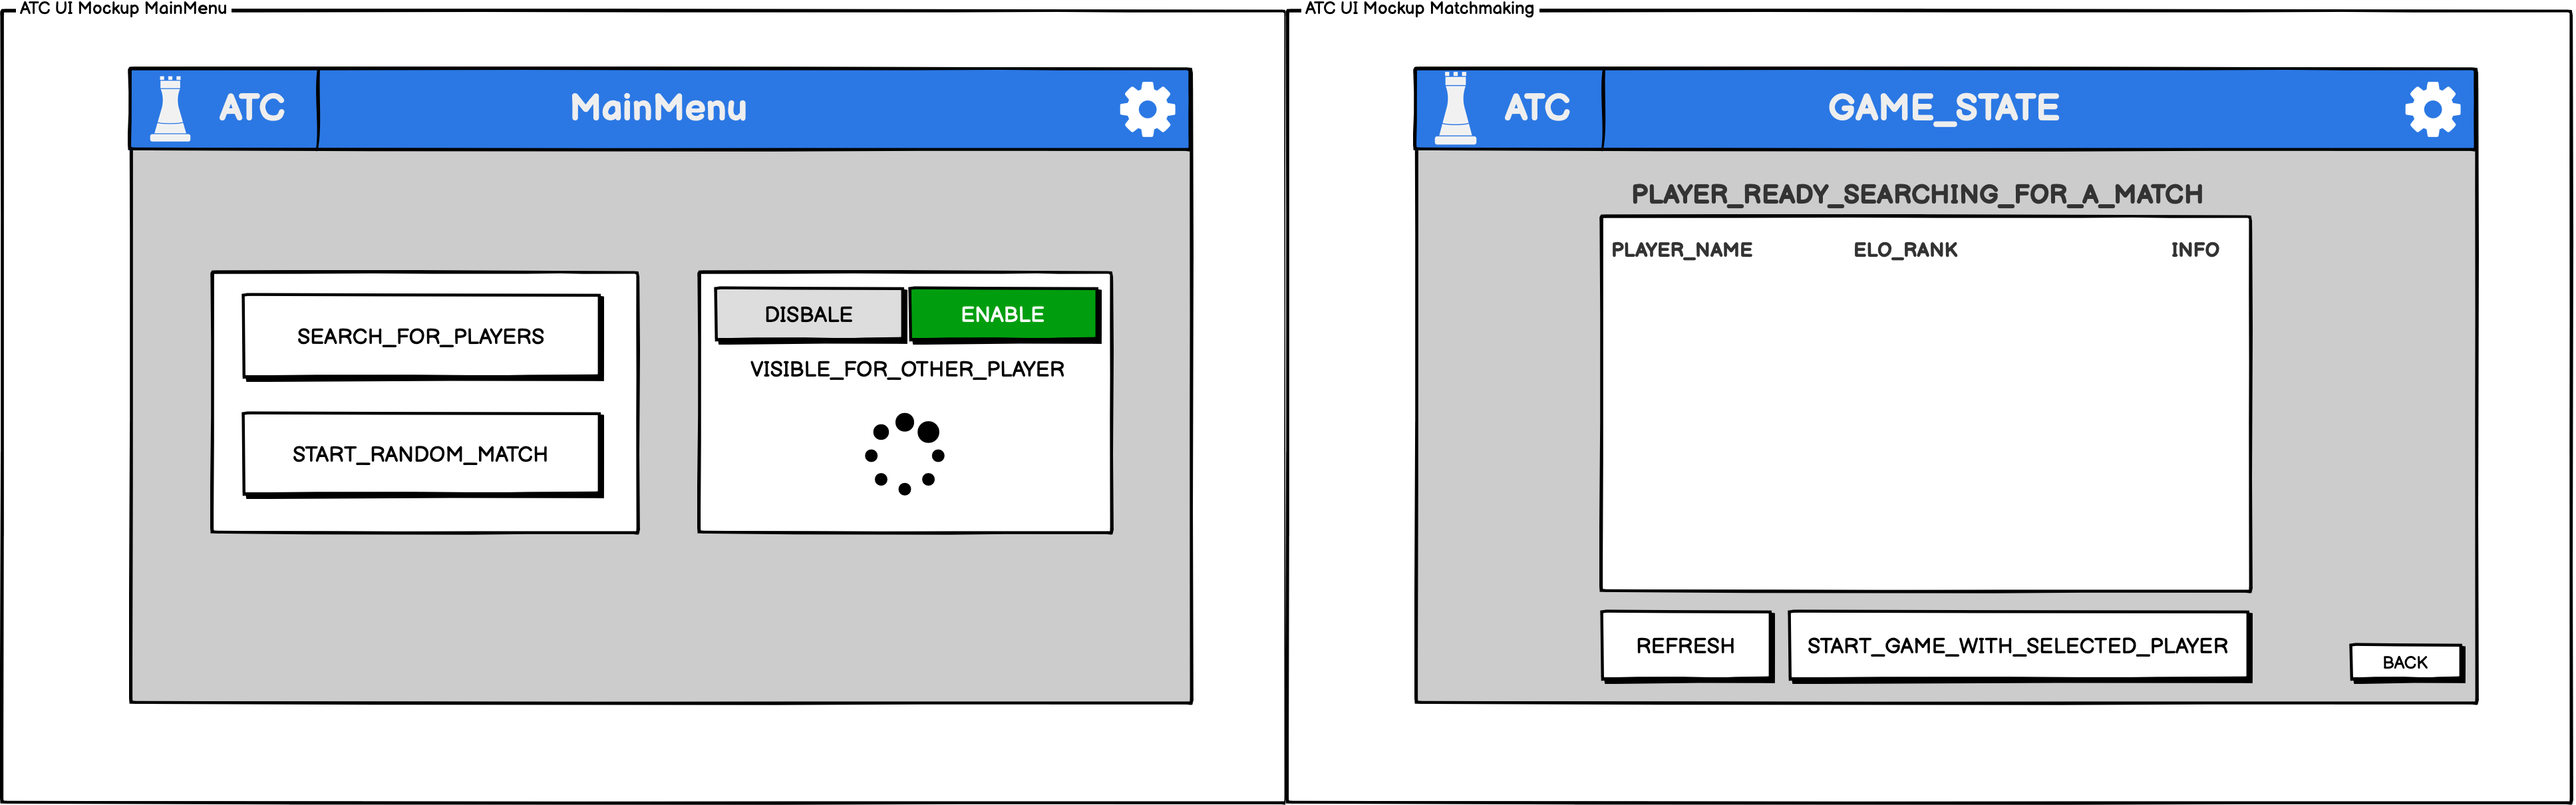
\includegraphics{images/ATC_Gui.png}
\caption{Embedded System Software: User-Interface Mockup
\label{ATC_Gui}}
\end{figure}

Das Qt\cite{qtframework} bietet dazu einen separaten Editor
\passthrough{\lstinline!Qt Design Studio!} an, in denen die zuvor
erstellen Wireframe-Grafiken importiert wurden und anschliessen mit den
Bedienelementen ersetzt werden könnten. Dieser Prozess gestaltete sich
als sehr effizient und so konnte das komplette UI mit moderatem
Zeitaufwand umgesetzt werden.

\begin{lstlisting}
// WINDOW.qml User-Interface ATC
import QtQuick 2.15
import QtQuick.Controls 2.15
//...
Rectangle {
    id: window
    objectName: "window"
    width: 800
    height: 480
    //BACKEND LOGIC INIT => CREATES INSTANCE OF THE MenuManager CLASS
    MenuManager{
        id:main_menu
        objectName: "mainmenu"
    }
    //...
    // MAIN MENU CONTAINER
    Rectangle {
        id: mm_container
        objectName: "mm_container"
        property var headline_bar_name:"Main Menu"
        //START AI MATCH BUTTON
        Button {
                id: mm_start_random_btn
                x: 40
                y: 183
                width: 207
                height: 55
                text: qsTr("START AI MATCH")
                //CONNECT BUTTON EVENTS TO BACKEND LOGIC
                Connections {
                    target: mm_start_random_btn
                    function onClicked(_mouse){
                        //CALL A FUNCTION IN BACKEND LOGIC INSTANCE
                        main_menu.mm_search_for_players_toggled(true)
                    }
                    //...
                }
                //...
\end{lstlisting}

Die anschließende Implementierung der Backend-Logik des Unter-Interface
bestand in der Verbindung, der in QML erstellten Bedienelemente durch
den \passthrough{\lstinline!Qt Design Studio!}-Editor und der
User-Interface Backend Logik. Diese beschränkt sich auf die
Initialisierung des Fensters und dem anschließenden laden und darstellen
des QML Codes. Die Backend-Logik Funktionalitäten in einem QML Typ
\passthrough{\lstinline!MenuManager!} angelegt, welcher vor dem Laden
des eigentlichen User-Interface QML Codes registriert werden muss.

\begin{lstlisting}[language={C++}]
// main.cpp User-Interface ATC
#include <QGuiApplication>
#include <QQmlApplicationEngine>
#include "menumanager.h" //BACKEND LOGIC
int main(int argc, char *argv[])
{
  QCoreApplication::setAttribute(Qt::AA_EnableHighDpiScaling);
  //...
  //CREATE WINDOW
  QWindow window;
  window.setBaseSize(QSize(800,480));

  //REGISTER MainMenu COMPONENT
  qmlRegisterType<MenuManager>("MenuManager",1,0,"MenuManager");
  //LOAD User-Interface QML
  QQuickView view;
  //...
  view.engine()->addImportPath("qrc:/qml/imports");
  view.setSource(QUrl("qrc:/qml/WINDOW.qml"));
  view.engine()->rootContext()->setContextProperty("app", &app);
  //...
  //IMPORTANT STEP: AFTER INIT THE MainMenu COMPONENT HAS NO PARENT
  //SO WE NEED TO SET IT MANUALLY TO MAKE C++ -> QML FUNCATION CALLS WORKING
  QObject *object = view.rootObject();
  QObject *rect = object->findChild<QObject*>("mainmenu");
  if (rect){
         rect->setParent(object);
  }
  //FINALLY SHOW MENU ON SCREEN
  view.show();
}
\end{lstlisting}

Da das User-Interface ein separates Programm ist, welches auf dem System
ausgeführt wird, muss dieses in der Lage sein mit der
Controller-Software zu kommunizieren. Hierzu wurde die zuvor erstellte
\gls{ipc} Bibliothek in das Projekt importiert, jedoch wurde in der
Makefile das \passthrough{\lstinline!USES\_QT!} Define-Flag gesetzt.
Wenn dieses gesetzt ist, wird die Bibliothek in den Client-Modus
versetzt und stellt somit das Gegenstück zu der Instanz dar, welche in
der Controller-Software läuft. Somit werden auch die Funktionen zum
Senden von \passthrough{\lstinline!gui.createEvent()!} umgekehrt, sodass
ein Event in der Controller-Software ausgelöst wird. Dies kann z.B.
durch eine Benutzereingabe oder wenn das User-Interface die von der
Controller-Software geforderten Zustand angenommen hat.

\begin{lstlisting}[language={C++}]
// menumanager.cpp User-Interface ATC
#include "menumanager.h"

MenuManager::MenuManager()
{
    //START IPC THREAD
    guiconnection.start_recieve_thread();
    //...
}

//METHOD CALLED FROM QML ELEMENT ss_calboard_btn
void MenuManager::ss_calboard_btn(){
    //SEND EVENT TO CONTROLLER SOFTWARE
    guiconnection.createEvent(guicommunicator::GUI_VALUE_TYPE::START_CALBOARD_PROC);
}

//PROCESSES EVENTS COMMING FROM THE INTER PROCESS COMMUNICATION AND SHOWS MENUS OR SET IMAGES/LABES
// MenuManager::updateProgress() CALLED BY SPERATE THREAD
void MenuManager::updateProgress()
{
    //GET LATEST EVENT FROM IPC
    const guicommunicator::GUI_EVENT ev =  guiconnection.get_gui_update_event();
    if(!ev.is_event_valid){return;}
    //PROCESS EVENTS
    //SWITCH MAIN MENU REQUEST
    if(ev.event == guicommunicator::GUI_ELEMENT::SWITCH_MENU){
        switch_menu(ev.type);
    }
    //...
}
\end{lstlisting}

\hypertarget{fazit}{%
\chapter{Fazit}\label{fazit}}

Zusammenfassend lässt sich feststellen, dass das Ziel der Arbeit
erreicht wurde. Es wurde ein Prototyp eines autonomen Schachtischs
entwickelt.

\begin{itemize}
\item
  mit am weitesten forgeschrittener open-source autonomes Schachtisch
  Projekt
\item
  vom versierten Benutzer selbstädig aufbaubar
\item
  leichte bedienung
\item
  lässt spiel für erweiterungen
\item
\end{itemize}

\hypertarget{ausblick}{%
\section{Ausblick}\label{ausblick}}

\begin{itemize}
\tightlist
\item
  Einbindung in existeirende Schach-Clouds z.B. https://lichess.org/
\item
  user-port für Erweiterungen (z.B. DGT Schachur)
\end{itemize}









%%%%%%%%%%%%%%%%%%%%%%%%%%%%%%%%%%%%%%%%%%%%%%%%%%%%%%%%%%%%
% REFERENZEN
%%%%%%%%%%%%%%%%%%%%%%%%%%%%%%%%%%%%%%%%%%%%%%%%%%%%%%%%%%%%
%% Verschiedene Versionen, nach DIN 1505 zu zitieren
\bibliographystyle{plaindin}
\bibliography{thesis_references}


%%%%%%%%%%%%%%%%%%%%%%%%%%%%%%%%%%%%%%%%%%%%%%%%%%%%%%%%%%%%
% ACRONYM VERZEICHNIS
%%%%%%%%%%%%%%%%%%%%%%%%%%%%%%%%%%%%%%%%%%%%%%%%%%%%%%%%%%%%
\printglossaries

%%%%%%%%%%%%%%%%%%%%%%%%%%%%%%%%%%%%%%%%%%%%%%%%%%%%%%%%%%%%
% ABBILDUNGSVERZEICHNIS
%%%%%%%%%%%%%%%%%%%%%%%%%%%%%%%%%%%%%%%%%%%%%%%%%%%%%%%%%%%%
\listoffigures

%%%%%%%%%%%%%%%%%%%%%%%%%%%%%%%%%%%%%%%%%%%%%%%%%%%%%%%%%%%%
% ABBILDUNGSVERZEICHNIS
%%%%%%%%%%%%%%%%%%%%%%%%%%%%%%%%%%%%%%%%%%%%%%%%%%%%%%%%%%%%
\listoftables

%%%%%%%%%%%%%%%%%%%%%%%%%%%%%%%%%%%%%%%%%%%%%%%%%%%%%%%%%%%%
% ANHANG
%%%%%%%%%%%%%%%%%%%%%%%%%%%%%%%%%%%%%%%%%%%%%%%%%%%%%%%%%%%%
\newpage
\appendix % ANHANG EINLEITEN
\hypertarget{anhang}{%
\section{Anhang}\label{anhang}}



\end{document}
